\documentclass[leqno, openany]{memoir}
\setulmarginsandblock{3.5cm}{3.5cm}{*}
\setlrmarginsandblock{3cm}{3.5cm}{*}
\checkandfixthelayout

\usepackage{amsmath}
\usepackage{amssymb}
\usepackage{amsthm}
%\usepackage{MnSymbol}
\usepackage{bm}
\usepackage{accents}
\usepackage{mathtools}
\usepackage{tikz}
\usetikzlibrary{calc}
\usetikzlibrary{automata,positioning}
\usepackage{tikz-cd}
\usepackage{forest}
\usepackage{braket} 
\usepackage{listings}
\usepackage{mdframed}
\usepackage{verbatim}
\usepackage{physics}
\usepackage{stmaryrd}
\usepackage{mathrsfs} 
\usepackage[normalem]{ulem} 
\usepackage{stackengine}
\usepackage{bbm}
%\usepackage{/home/patrickl/homework/macaulay2}

%font
\usepackage[sc]{mathpazo}
\usepackage{eulervm}
\usepackage[scaled=0.86]{berasans}
\usepackage{inconsolata}
\usepackage{microtype}

%CS packages
\usepackage{algorithmicx}
\usepackage{algpseudocode}
\usepackage{algorithm}

% typeset and bib
\usepackage[english]{babel} 
\usepackage[utf8]{inputenc} 
\usepackage[T1]{fontenc}
\usepackage[bookmarks, colorlinks, breaklinks]{hyperref} 
\hypersetup{linkcolor=blue,citecolor=magenta,filecolor=black,urlcolor=blue}
\usepackage{cleveref}
\usepackage[backend=biber,style=alphabetic,maxalphanames=4,maxnames=5,hyperref,backref=true,backrefstyle=none]{biblatex}
\usepackage{xpatch}
\xpatchbibmacro{pageref}{parens}{backrefparens}{}{}
\crefname{equation}{}{}

% other formatting packages
\usepackage{float}
\usepackage{booktabs}
\usepackage[shortlabels]{enumitem}
\usepackage{csquotes}
\usepackage{titlesec}
\usepackage{titling}
\usepackage{parskip}
\usepackage{graphicx}
\graphicspath{{./}}

\usepackage{lipsum}

% delimiters
\DeclarePairedDelimiter{\gen}{\langle}{\rangle}
\DeclarePairedDelimiter{\floor}{\lfloor}{\rfloor}
\DeclarePairedDelimiter{\ceil}{\lceil}{\rceil}


\newtheorem{thm}{Theorem}[section]
\newtheorem{cor}[thm]{Corollary}
\newtheorem{prop}[thm]{Proposition}
\newtheorem{lem}[thm]{Lemma}
\newtheorem{conj}[thm]{Conjecture}
\newtheorem{quest}[thm]{Question}
\newtheorem{prob}[thm]{Problem}

\theoremstyle{definition}
\newtheorem{defn}[thm]{Definition}
\newtheorem{defns}[thm]{Definitions}
\newtheorem{con}[thm]{Construction}
\newtheorem{exm}[thm]{Example}
\newtheorem{exms}[thm]{Examples}
\newtheorem{notn}[thm]{Notation}
\newtheorem{notns}[thm]{Notations}
\newtheorem{addm}[thm]{Addendum}
\newtheorem{exer}[thm]{Exercise}

\theoremstyle{remark}
\newtheorem{rmk}[thm]{Remark}
\newtheorem{rmks}[thm]{Remarks}
\newtheorem{warn}[thm]{Warning}
\newtheorem{sch}[thm]{Scholium}


% unnumbered theorems
\theoremstyle{plain}
\newtheorem*{thm*}{Theorem}
\newtheorem*{prop*}{Proposition}
\newtheorem*{lem*}{Lemma}
\newtheorem*{cor*}{Corollary}
\newtheorem*{conj*}{Conjecture}

% unnumbered definitions
\theoremstyle{definition}
\newtheorem*{defn*}{Definition}
\newtheorem*{exer*}{Exercise}
\newtheorem*{defns*}{Definitions}
\newtheorem*{con*}{Construction}
\newtheorem*{exm*}{Example}
\newtheorem*{exms*}{Examples}
\newtheorem*{notn*}{Notation}
\newtheorem*{notns*}{Notations}
\newtheorem*{addm*}{Addendum}


\theoremstyle{remark}
\newtheorem*{rmk*}{Remark}

% shortcuts
\newcommand{\Ima}{\mathrm{Im}}
\newcommand{\A}{\mathbb{A}}
\newcommand{\F}{\mathbb{F}}
\newcommand{\E}{\mathcal{E}}
\newcommand{\G}{\mathbb{G}}
\newcommand{\N}{\mathbb{N}}
\newcommand{\R}{\mathbb{R}}
\newcommand{\C}{\mathbb{C}}
\newcommand{\Z}{\mathbb{Z}}
\newcommand{\Q}{\mathbb{Q}}
\renewcommand{\k}{\Bbbk}
\renewcommand{\L}{\mathbb{L}}
\renewcommand{\P}{\mathbb{P}}
\newcommand{\M}{\overline{M}}
\newcommand{\g}{\mathfrak{g}}
\newcommand{\h}{\mathfrak{h}}
\newcommand{\n}{\mathfrak{n}}
\renewcommand{\b}{\mathfrak{b}}
\newcommand{\ep}{\varepsilon}
\newcommand*{\dt}[1]{%
   \accentset{\mbox{\Huge\bfseries .}}{#1}}
\renewcommand{\abstractname}{Official Description}
\newcommand{\mc}[1]{\mathcal{#1}}
\newcommand{\T}{\mathbb{T}}
\newcommand{\mf}[1]{\mathfrak{#1}}
\newcommand{\mr}[1]{\mathrm{#1}}
\newcommand{\ms}[1]{\mathsf{#1}}
\newcommand{\mt}[1]{\mathtt{#1}}
\newcommand{\on}[1]{\operatorname{#1}}
\newcommand{\ol}[1]{\overline{#1}}
\newcommand{\ul}[1]{\underline{#1}}
\newcommand{\wt}[1]{\widetilde{#1}}
\newcommand{\wh}[1]{\widehat{#1}}
\renewcommand{\div}{\operatorname{div}}
\newcommand{\bir}{\sim_{\mr{bir}}}
\newcommand{\stacks}[1]{\href{https://stacks.math.columbia.edu/tag/#1}{#1}}
\newcommand{\ostar}{\stackMath\mathbin{\stackinset{c}{0ex}{c}{0ex}{\star}{\bigcirc}}}

\DeclareMathOperator{\Der}{Der}
\DeclareMathOperator{\Def}{Def}
\DeclareMathOperator{\Bl}{Bl}
\DeclareMathOperator{\NE}{NE}
\DeclareMathOperator{\Tor}{Tor}
\DeclareMathOperator{\Hom}{Hom}
\DeclareMathOperator{\Ext}{Ext}
\DeclareMathOperator{\End}{End}
\DeclareMathOperator{\ad}{ad}
\DeclareMathOperator{\Aut}{Aut}
\DeclareMathOperator{\Rad}{Rad}
\DeclareMathOperator{\Pic}{Pic}
\DeclareMathOperator{\supp}{supp}
\DeclareMathOperator{\Supp}{Supp}
\DeclareMathOperator{\sgn}{sgn}
\DeclareMathOperator{\spec}{Spec}
\DeclareMathOperator{\Spec}{Spec}
\DeclareMathOperator{\proj}{Proj}
\DeclareMathOperator{\Proj}{Proj}
\DeclareMathOperator{\ord}{ord}
\DeclareMathOperator{\Div}{Div}
\DeclareMathOperator{\depth}{depth}
\DeclareMathOperator{\coker}{coker}
\DeclareMathOperator{\codim}{codim}
\DeclareMathOperator{\ch}{ch}
\DeclareMathOperator{\Hilb}{Hilb}

% Section formatting
\titleformat{\section}
    {\Large\sffamily\scshape\bfseries}{\thesection}{1em}{}
\titleformat{\subsection}[runin]
    {\large\sffamily\bfseries}{\thesubsection}{1em}{}
\titleformat{\subsubsection}[runin]{\normalfont\itshape}{\thesubsubsection}{1em}{}

\title{COURSE TITLE}
\author{Lectures by INSTRUCTOR, Notes by NOTETAKER}
\date{SEMESTER}

\newcommand*{\titleSW}
    {\begingroup% Story of Writing
    \raggedleft
    \vspace*{\baselineskip}
    {\Huge\itshape Simons Math Summer Workshop 2023}\\[\baselineskip]
    {\large\itshape Notes by Patrick Lei}\\[0.2\textheight]
    {\Large Lectures by Various}\par
    \vfill
    {\Large \sffamily Simons Center for Geometry and Physics}
    \vspace*{\baselineskip}
\endgroup}
\pagestyle{simple}

\chapterstyle{ell}


%\renewcommand{\cftchapterpagefont}{}
\renewcommand\cftchapterfont{\sffamily}
\renewcommand\cftsectionfont{\scshape}
\renewcommand*{\cftchapterleader}{}
\renewcommand*{\cftsectionleader}{}
\renewcommand*{\cftsubsectionleader}{}
\renewcommand*{\cftchapterformatpnum}[1]{~\textbullet~#1}
\renewcommand*{\cftsectionformatpnum}[1]{~\textbullet~#1}
\renewcommand*{\cftsubsectionformatpnum}[1]{~\textbullet~#1}
\renewcommand{\cftchapterafterpnum}{\cftparfillskip}
\renewcommand{\cftsectionafterpnum}{\cftparfillskip}
\renewcommand{\cftsubsectionafterpnum}{\cftparfillskip}
\setrmarg{3.55em plus 1fil}
\setsecnumdepth{subsection}
\maxsecnumdepth{subsection}
\settocdepth{subsection}

\addbibresource{../../math.bib}
\DefineBibliographyStrings{english}{
    backrefpage={$\leftarrow$},
    backrefpages={$\leftarrow$},
}

\begin{document}
    
\begin{titlingpage}
\titleSW
\end{titlingpage}

\thispagestyle{empty}
\section*{Disclaimer}%
\label{sec:disclaimer}

These are my notes from the second and third weeks of the 2023 Simons Math Summer Workshop.

These notes were taken during the lectures using \texttt{neovim}. 
Any errors are mine and not the speakers'. 
In addition, my notes are picture-free (but will include commutative diagrams) and are a mix of my mathematical style and that of the lecturers. Also, notation may differe between lecturers.
If you find any errors, please contact me at \texttt{plei@math.columbia.edu}.

\section*{Acknowledgements}

I would like to thank Mark Gross, Mark McLean, Simon Donaldson, Kenji Fukaya, John Pardon, and the Simons Center for organizing the workshop.

\vspace*{1cm}

\noindent\textbf{Program Website:}  \url{https://scgp.stonybrook.edu/archives/39185}
\newpage

\tableofcontents

\chapter{Degenerations of holomorphic curves, tropical geometry, gluing theorems, and exploded manifolds (Brett Parker)}%
\label{cha:parker}

\section{Geometry of holomorphic curves}

Consider a map $f \colon \Sigma \to M$, where $\Sigma$ is a Riemann surface and $M$ is a manifold with metrics $g_{\Sigma}, g_M$ respectively.

\begin{defn}
    The \textit{$L^2$ energy} of $f$ is given by
    \[ L^2(f) \coloneqq \int_{\Sigma} \frac{1}{2} \abs{Df}^2 \dd{A}, \]
    where $\abs{Df}$ is defined using $g_{\Sigma}$ and $g_M$ on $T^*\Sigma \otimes TM$.
\end{defn}

This is conformally invariant, as can be seen by computing the energy after scaling $g_{\Sigma}$. This is also analogous to the definition of geodesics, where we consider stationary points of
\[ L(\gamma) = \int \frac{1}{2} \abs{\dot{\gamma}}^2 \dd{t}. \]

We really want to consider holomorphic maps, so we choose an almost complex structure $J \in \End(TM)$ such that
\[ g(J-, J-) = g(-,-). \]
This defines a 2-form by
\[ \omega(v,w) \coloneqq g(Jv, w), \]
which is not necessarily closed. We also choose a complex structure $j$ on $\Sigma$.

\begin{lem}
    The $L^2$ energy of $f$ satisfies the inequality
    \[ L^2(f) \geq \on{Area}(f) \geq \int_{\Sigma} f^* \omega \]
    with inequality if and only if $\dd{f} \circ j = J \circ \dd{f}$ (meaning that $f$ is holomorphic).
\end{lem}

Locally, if we choose coordinates $x,y$ such that the complex structure is $x+iy$, then
\begin{align*} 
    \int_{\Sigma} f^* \omega &= \int_{\Sigma} g(J f_x, f_y) \dd{x} \wedge \dd{y} \\
    &\leq \int_{\Sigma} \qty(\frac{1}{2} \abs{f_x}^2 + \frac{1}{2} \abs{f_y}^2) \dd{x} \dd{y},
\end{align*}
with equality if and only if $f$ is holomorphic.

\begin{rmk}
    It is tempting to consider just the area in the inequality, but that would not tell us how to parameterize the curve, just like how defining geodesics by minimizing length doesn't tell us how to parameterize the geodesic.
\end{rmk}

If $\omega$ is closed, then $E_{\omega}(f) = \int_{\Sigma} f^*\omega$ is deformation invariant, so $f$ is holomorphic if and only if $f$ minimizes $L^2$-energy and $L^2(f) = E_{\omega}(f)$.

\subsection{Regularity}


\begin{lem}[Monotonicity]
    Consider a ball of radius $R$ such that a nonconstant holomorphic curve $f$ passes through its center. Then
    \[ L^2\qty(f|_{f^{-1}(B_R(f(z_0)))}) \geq \ep_R, \]
    where $\ep_R$ depends on $g_M$ and $R$.
\end{lem}

Morally, we should think that it takes some amount of energy for our curve to escape the ball.

Now note that the Cauchy-Riemann equation is elliptic, so we have elliptic regularity. Specifically, we have
\[ \sup_{B_{\frac{1}{2}}(0)} \abs{D^k f} \leq c_k \sup_{B_1(0)} \abs{Df}, \]
which gives us bounds on all higher derivatives, so solutions are smooth. Unfortunately, $L^2$ energy bounds do not guarantee derivative bounds.

\begin{thm}[Removable singularity]
    If $L^2(f) < \infty$ then $f \colon \Sigma \setminus p$ extends over $p$.
\end{thm}

\begin{lem}
    Consider $f \colon B_1(0) \to M$. If $L^2(f)$ is small, then
    \[ \abs{Df(0)} \leq c. \]
\end{lem}

\subsection{Think-thin decomposition of the domain}

For a holomorphic curve $f \colon \Sigma \to M$ with $E_{\omega}(f) < \omega$, our goal is to decompose $\Sigma$ into long thin annuli $A$ with low energy and ``thick'' regions $C_i$ such that
\begin{itemize}
    \item $E_{\omega}(f|_A) < \ep_0$;
    \item $\abs{df}$ is bounded on $C$;
    \item The diameters of the $C_i$ are bounded;
    \item Either $\chi(C_i) < 0$ or $E_{\omega}(f|_{C_i}) > \ep_0$.
\end{itemize}

\begin{rmk}
    This requires changing the metric in the same conformal class to eliminate bubbling.
\end{rmk}

Taking the limit as the lengths of the annuli go to infinity, we obtain a degerated holomorphic curve with many components.

\subsection{Noncompact stuff}

Some examples of noncompact manifolds we want to consider are $N \times \underbrace{\R \times S^1}_{\C^{\times}}$, where $N$ is compact, or $(\C^{\times})^k \rtimes N$, where the fibers are holomorphic and $J, g$ are $\C^{\times}$-invariant. In the first case, we are using a $\C^{\times}$-invariant metric, so the manifold really does look like a cylinder. A third case we will consider are those which are asymptotically cylindrical, for example $M \setminus D$, where $M$ is a complex manifold and $D$ is a normal crossings divisor.

In these cases, we must use a different taming form $\omega$, so $g \neq \omega(-, J-)$. For example, in the cylindrical case we can consider
\[ \omega = \omega_N + \sum_h \dd{\rho_h(t_h)} \alpha_h, \]
$\alpha_h$ is a connection form, $t, \theta$ are coordinates on $\R \times S^1$, and $\rho_h$ looks like a smoothed step function. We obtain the inequality
\[ E_{\omega} \geq L^2(\text{$f$ projected to $N$}) \]
or we consider the $L^2$ energy of $f$ locally on $(\C^{\times})^k \rtimes N$. Unfortunately, this means we only have local energy bounds.

\begin{exer}
    Let $f \colon A \to \C^{\times}$ be holomorphic with $\abs{\frac{\dd{f}}{f}} < c_0$. Write $A = \qty{e^{-T} \leq \abs{z} \leq e^T}$. Show that
    \begin{enumerate}[(a)]
        \item $\abs{\frac{\dd{f(z)}}{(f(z))} - \frac{\dd{f(1)}}{f(1)}} \leq e^{-T} c_0\qty(\abs{z} + \frac{1}{\abs{z}})$;
        \item $f(z) = e^{h(z)} a z^m$ with $h(z) \leq 2 \qty(\abs{z} + \frac{1}{\abs{z}}) e^{-T} c_0$.
    \end{enumerate}
\end{exer}

Therefore, in logarithmic coordinates, a holomorphic curve in $(\C^{\times})^2$ has its thin regions travelling in straight lines and the thick regions are very small. In the tropical limit, we obtain a piecewise-linear curve.

In all of these cases, we can replace the RHS of the first part of the exercise with
\[ e^{-\delta T} c_0 \qty(\abs{z_0}^{\delta} + \frac{1}{\abs{z_0}^{\delta}}), \]
where $0 < \delta < 1$.

\section{Exploded manifolds}
\label{sec:exploded}

One of the problems that we have is dealing with what happens in our moduli spaces as things go off to infinity. Of course, the moduli space of the tropical curves is not compact, but it is relatively nice. To deal with the problem in the usual geometry, we will develop the formalism of exploded manifolds.

\subsection{Explosion}
\label{subsec:explosion}

Let $R$ be a ring. The \textit{exploded semiring} is $Rt^{\R}$ with multiplication given by
\[ c_1 t^{a_1} c_2 t^{a_2} = c_1c_2 t^{a_1+a_2} \]
and addition given by
\[ c_1 t^{a_1} + c_2 t^{a_2} = \begin{cases}
                                 c_1 t^{a_1} & a_1 < a_2 \\
                                 (c_1 + c_2) t^{a_1} & a_1 = a_2 \\
                                 c_2 t^{a_2} & a_1 > a_2.
                               \end{cases}
\]

If $R$ is the ring with one element, then we get the tropical numbers. Then there is a \textit{tropical part homomorphism}
\[ R t^{\R} \to t^{\R} \qquad \ul{ct^a} = a, \]
where $a$ represents the tropical number $0t^a \in t^{\R}$. There is also a \textit{smooth part homomorphism}
\[ R t^{[0, \infty)} \to R \qquad \ceil{ct^a} = c \delta_{a,0}. \]

The goal is to define the functor
\[ \ms{Expl} \colon \ms{log} \to \ms{Exploded\ manifolds}. \]
First, we will define the \textit{exploded point}
\[ p^{\dag} = \Spec([0, \infty) \to \C) = (\Spec \C, \C^{\times}t^{[0, \infty)}). \]
For any log-scheme $X^{\dag}$, we will define
\[ \ms{Expl}(X^{\dag}) = X^{\dag} \times p^{\dag} = (X, \mc{M}_X t^{[0, \infty)}). \]
Here, the structure morphisms to $\mc{O}_X$ are as expected. A \textit{holomorphic morphism} of these exploded objects is simply a morphism $X^{\dag} \times p^{\dag} \to Y^{\dag} \times p^{\dag}$ over $p^{\dag}$.

\begin{exm}
  We will now consider the points $p^{\dag} \to \ms{Expl}(\C, 0)$. These correspond to morphisms
  \begin{equation}
    \begin{tikzcd}
      \mc{M}_{(C, 0)} t^{[0, \infty)} \ar{d}{h} \ar{r} & \mc{O}_{\C} \ar{d} \\
      \C^{\times} t^{[0, \infty)} \ar{r} & \C.
    \end{tikzcd}
  \end{equation}
  This is determined by the value $h(zt^0) \in \C^{\times}t^{[0, \infty)}$. We may now consider a new coordinate $\wt{z}$ on $\ms{Expl}(\C, 0)$. Thus, as a set, we have
  \[ \ms{Expl}(\C, 0) = \C^{\times}t^{[0, \infty)}. \]
  This will admit the notion of a tangent space and a metric, and geometrically we will see $\C \setminus 0$ with a cylindrical end at $0$ and then infinitely many cylindrical ends in the $[0, \infty)$ direction.
\end{exm}

\subsection{Exploded manifolds}
\label{subsec:exploded_mflds}

Changing perspective, we will consider $\ms{Expl}(\C, 0)$ as an exploded manifold. We will have
\begin{itemize}
\item A set of points $\C^{\times}t^{[0, \infty)}$;
\item A topology induced from the analytic topology on $\C$ using the smooth part homomorphism;
\item A sheaf of functions valued in $\C^{\times}t^{\R}$. These functions will look something like $f(\ceil{\wt{z}}) \wt{z}^m t^a$, where $m \in \Z$, $a \in \R$, and $f \colon \C \to \C^{\times}$ which is regular in some sense.
\end{itemize}

Here, regular could mean holomorphic, smooth, $C^k$, or another form of regularity known as $C^{\infty, \ul{1}}$. This means that for all $\delta < 1$, the function $\abs{f(z) - f(0)} \abs{z}^{-\delta}$ extends to be continuous at $0$ and so do all of its derivatives $\abs{D^kf(z)} \abs{z}^{-\delta}$, where the deriatives are defined using the real or imaginary parts of $z \pdv{z}$.

\begin{defn}
  An \textit{exploded space} $B$ is a set $B$ equipped with
  \begin{itemize}
  \item A topology induced from a surjective map $B \to \ceil{B}$, where $\ceil{B}$ is Hausdorff;
  \item A sheaf of $\C^{\times} t^{\R}$-valued functions $\mc{E}^{\times}(B)$ containing constants.
  \end{itemize}
\end{defn}

\begin{exm}
For the exploded manifold $\ms{Expl}(X^{\dag})$, then the set $B$ is the set of maps $p^{\dag} \to X^{\dag}$, the smooth part is $\ceil{\ms{Expl}(X^{\dag})} = X$ with the analytic topology, and $\mc{E}^{\times}(\ms{Expl}(X^{\dag})) = \mc{M}_X^{\mr{gp}} t^{\R}$.
\end{exm}

\begin{exm}
We will consider an important non-logarithmic example. We will consider $\mathbb{T} = \C^{\times}t^{\R}$ with $\ceil{\mathbb{T}} = \mr{pt}$ and $\mc{E}^{\times}(\mathbb{T})$ the set of monomials $ct^az^m$.
\end{exm}

\begin{exer}
Show that for any exploded space $B$, maps $B \to \T$ correspond to sections of $\mc{E}^{\times}(B)$.
\end{exer}

\begin{exm}
  The most general example will be $\mathbb{T}^m_P$, where $P \subset \R^m$ is an integral affine polytope defined by inequalities of the form $\alpha \cdot x + a \geq 0$, where $\alpha \in \Z^m$ and $a \in \R$. We also allow strict inequalities. We will define the set $\mathbb{T}^m_P \subset (\C^{\times}t^{\R})^m$ as the points whose tropical part lie in $P$.

  We will now set 
  \[ M = \Hom(P, [0, \infty))/ \Hom(P, (0, \infty)) \]
  to be the quotient of integral affine maps on $\R^m$ that are nonnegative on $P$ by those which are strictly positive. As a log scheme, this is
  \[ \Spec(\Hom(P, [0, \infty)) \to \C[M]). \]
  Note that $M$ is finitely generated. Writing an integral affine map $\alpha \cdot x + a$, we can write the monomial $z^{\alpha}t^a$, and this gives us $\zeta = \ceil{z^{\alpha}t^a}$. Choosing generators for $M$, we have a map $\mathbb{T}_P \to \C^k$ given by $(\zeta_1, \ldots, \zeta_k)$. The image of this map will be called $\ceil{\mathbb{T}_P}$.

  Finally, we can write
  \[ \mc{E}^{\times}(T^m_P) = \qty{h(\zeta_1, \ldots, \zeta_k)z^{\alpha}t^a}, \]
  where $h \colon \C^k \to \C^{\times}$ is regular.
\end{exm}

More generally, our coordinate charts for exploded manifolds will be $\R^k \times \mathbb{T}_P^m$, where the smooth part and sheaf of exploded functions are as expected.

\begin{exm}
  One relatively simple example is $\T^m_{[0, \infty)^m} = \ms{Expl}(\C, 0)^m$.
\end{exm}

\begin{exm}
Another simple example is $\T^1_{(0, \infty)} = \ms{Expl}(\Spec \N \to \C)$.
\end{exm}

\begin{defn}
An \textit{exploded manifold} is an exploded space which is locally isomorphic to $\R^k \times \mathbb{T}_P^m$.
\end{defn}

\begin{exer}\leavevmode
  \begin{enumerate}[(a)]
  \item Maps $f \colon B \to \T_Q^n$ correspond to $n$-tuples $f_1, \ldots, f_n \in \mc{E}^{\times}(B)$ such that $(\ul{f}) \in Q$;
  \item Maps $\T_P^m \to \T_Q^n$ correspond to integral maps $f \colon P \to Q$;
    \item Maps $f \colon B \to \R$ correspond to global sections $f^{-1}(e^xt^0) \in \mc{E}^{\times}(B)$ valued in $\R^{>0}t^0$, which are the same as regular maps $\ceil{B} \to \R$.
  \end{enumerate}
\end{exer}

\begin{exm}
  We will now consider the example of a compact polytope. As a set, we have
  \[ \T^1_{[0,\ell]} = \C^{\times}t^{[0,\ell]}. \]
  Geometrically, the copies of the $\C^{\times}$ will be asympotically cylindrical only at one end. Note that the $M$ here is generated by two elements (zero at one of the two endpoints), where $\zeta_1 = \ceil{z}$ and $\zeta_2 = \ceil{z^{-1}t^{\ell}}$. Next, we note that
  \[ \ceil{\T^1_{[0,1]}} = (\zeta_1 \zeta_2 = 0) \subset \C^2, \]
  which is the model for a node.
\end{exm}

\begin{exer}
Show that $\mathbb{T}^1_{[0,\ell]} = \qty{z_1z_2 = t^{\ell}} \subseteq \mathbb{T}^2_{[0, \infty)} = \ms{Expl}(\C, 0)^2$.
\end{exer}
Note that there is a map $\ms{Expl}(\C, 0)^2 \xrightarrow{z_1z_2} \ms{Expl}(\C, 0)$, and so we see $\T^1_{[0,1]}$ as a fiber of this map.

\subsection{Geometric structures}
\label{subsec:geometry}



As usual, vector fields will correspond to real derivations on $\mc{E}(B)$, which is a sheaf of (semi)-rings. Recall that a derivation $v$ must be linear and satisfy the Leibniz rule:
\begin{align*}
  v(f+g) &= v(f) + v(g) \\
  v(fg) &= v(f) g + f v(g).
\end{align*}
Then the condition of being real means that if $f$ is $\R t^{\R}$-values, so is $v(f)$. We also require that
\[ v(ct^a) = 0 t^a \]
for constant functions. For example, there is an isomorphism
\[ T \T_P^m \cong \R^{2m} \times \T_P^m \]
generated by the vector fields
\[ \Re \qty[z_i \pdv{z_i}], \Im \qty[z_i \pdv{z_i}]. \]

\begin{defn}
  A vector $v \in {}^{\Z}T_p B \subset T_p B$ is \textit{integral} if $\frac{vf}{f} \in \Z$ for all $f \in \E^{\times}(B)$.
\end{defn}

\begin{defn}
An \textit{almost complex structure} $J$ is a regular section of $T^*B \otimes TB$ such that $J^2 = - \mr{Id}$ and $(Jv) f = i(vf)$ for any $v \in {}^{\Z}T_p B$.
\end{defn}

\begin{defn}
An exploded manifold $B$ is \textit{complete} if $\ceil{B}$ is compact and locally isomorphic to $\R^n \times \T_p^m$ for a closed polytope $P$.
\end{defn}

\section{Families of exploded curves}
\label{sec:families}

\subsection{Exploded curves}
\label{subsec:curves}

\begin{defn}
A \textit{curve} $C$ is a complete, $2$-dimensional exploded manifold with an almost complex structure. A \textit{regular curve} in an almost complex exploded manifold $(B, J)$ is a regular map $f \colon C \to B$ from a curve. Such an $f$ is \textit{holomorphic} if $\dd{f} \circ j = J \circ \dd{f}$.
\end{defn}

The local models for exploded curves are open subsets of:
\begin{itemize}
\item $\C$, corresponding to regular points;
\item $\T^1_{[0, \ell]}$, corresponding to nodes;
\item $\T^1_{[0, \infty)}$, corresponding to ends.
\end{itemize}
The underlying topological space $\ceil{C}$ is simply a nodal curve, while the tropical part will have vertices corresponding to smooth components, edges corresponding to nodes, and infinite legs corresponding to the ends. At every node, we will have an extra choice of $\C^{\times} t^{(0, \infty)}$ gluing information, which makes the tropical part a metric graph.

Automorphisms of holomorphic curves are holomorphic automorphisms $h \colon C \to C$ which commute with $f$. These induce automorphisms of $\ceil{f}$, but not every automorphism of $\ceil{f}$ respects the gluing data, so they may not lift. Thus there are exploded curves with finite automorphism group as curves, but whose underlying curves are not stable.

\begin{defn}
A curve $f$ is \textit{stable} if the automorphism group $\Aut \ceil{f}$ is finite.\footnote{This is automatically satisfied if $C = \T$.}
\end{defn}

\subsection{Families}
\label{subsec:families}

\begin{defn}
  A \textit{family} $\Pi \colon \wh{B} \to B_0$ is a complete map such that for all $p \in \wh{B}$, the maps
  \[ T_p \Pi \colon T_p \wh{B} \to T_p B_0, \qquad T_p \Pi \colon {}^{\Z}T_p \wh{B} \to {}^{\Z}T_p B_0 \]
  are surjective.
\end{defn}

For example, the explosion of any normal crossings degeneration is a family in our sense.

\begin{defn}
  A \textit{regular family} of curves $\wh{f}$ in a family $\wh{B}$ is a regular commutative diagram
  \begin{equation*}
    \begin{tikzcd}
      (C(\wh{f}), j) \ar{r}{\wh{f}} \ar{d} & (\wh{B}, J) \ar{d} \\
      F(\wh{f}) \ar{r} & B_0
    \end{tikzcd}
  \end{equation*}
  such that the left arrow is a family whose fibers are curves.
  A \textit{morphism} $\alpha \colon \wh{g} \to \wh{f}$ is a pullback diagram
  \begin{equation*}
    \begin{tikzcd}
      C(\wh{g}) \ar{d} \ar{r} \ar[bend left=20]{rr}{\wh{g}} & C(\wh{f}) \ar{d} \ar[swap]{r}{\wh{f}} & \wh{B} \ar{d} \\
      F(\wh{g}) \ar{r} & F(\wh{f}) \ar{r} & B_0.
    \end{tikzcd}
  \end{equation*}
\end{defn}

Using this, we may define the moduli stack $\mc{M}^{\infty, 1}(B)$ of $C^{\infty, 1}$ curves in $B$. Then there is a sequence of inclusions
\[ \mc{M} \overset{\text{closed}}{\subset} \mc{M}^{\mr{st}} \overset{\text{open}}{\subset} \mc{M}^{\infty, 1}(B), \]
where $\mc{M}$ is stable holomorphic curves and $\mc{M}^{\mr{st}}$ is $C^{\infty, 1}$ stable curves. This carries a topology, where an open substack $U \subset \mc{M}^{\infty, 1}$ is such that its preimage $U(\wh{f}) \subset F(\wh{f})$ is open and for any morphism $\alpha \colon \wh{f} \to \wh{g}$, $F(\alpha)^{-1} U(\wh{g}) = U(\wh{f})$.

\subsection{Gromov compactness}
\label{subsec:gromov_compactness}

Given an appropriate taming form $\omega$ on $B$, the open substack
\[ \mc{M}_{g, n, E} \subset \mc{M}^{\infty,1} \]
of stable curves with at most a prescribed energy $E$ is in fact compact. Equivalently, any sequence of $\mc{M}_{g, n, E}$ has a subsequence $f_i$ such that there exists a regular family $\wh{f}$ and maps $\alpha_i \colon f_i \to \wh{f}$ such that $\ceil{ F(\alpha) } \subset \ceil{ F(\wh{f}) }$ converges.

\subsection{Kuranishi structure}
\label{subsec:kuranishi}

Recall that $T_f \mc{M}^{\mr{st}}$ give first-order deformations of $f$. We can also consider
\[ \ol{\partial} f = \frac{1}{2}(\dd{f} + J \circ \dd{f} \circ j), \]
which is a section of $Y(f) = (T^* C \otimes f^* TB)^{0,1}$ that vanishes on the edges of $C$. We will call the sections of this $\mc{Y}(f)$ and this is a vector bundle on $\mc{M}^{\mr{st}}$. For any holomorphic $f$, we obtain a linearization
\[ D_f \ol{\partial} \colon T_f \mc{M}^{\mr{st}} \to \mc{Y}(f) \]
of the $\ol{\partial}$-equation.

\begin{thm}
If $D_f \ol{\partial}$ is surjective, then there exists an open neighborhood $U \subset \mc{M}^{\mr{st}}$ of $f$ and a regular family $\wh{f} \subset U$ with finite automorphism group $G$ such that $\mc{M} \cap U = \wh{f} / G$.
\end{thm}
Therefore, when we have transversality, the moduli space is an exploded orbifold. Unfortunately, this does not always hold.

\begin{thm}
For an arbitrary $f \in \mc{M}$, there exists an open $U \subset \mc{M}^{\mr{st}}$ and a nice finite rank $V \subset \mc{Y}$ over $U$, $\wh{f} \subset U$, and $G$ as above such that $\ol{\partial}^{-1}(V) = \wh{f} / G$ and and $\mc{M} \cap U = \ol{\partial}^{-1}(0)$.
\end{thm}

\subsection{Refinements}
\label{subsec:label}

\begin{defn}
A \textit{refinement} of an exploded manifold $B$ is a complete, bijective submersion $B' \to B$.\footnote{Note that for ordinary manifolds, this is simply a diffeomorphism.}
\end{defn}

If we consider the fiber product diagram
\begin{equation*}
  \begin{tikzcd}
    B' \ar{d}{\mr{id}} \ar{r}{\mr{id}} & B' \ar{d} \\
    B' \ar{r} & B,
  \end{tikzcd}
\end{equation*}
of a refinement with itself, it must always look like the above.

\begin{exm}
  Let $(X^n, D)$ be a compact toric variety. Then there is a refinement map
  \[ \ms{Expl}(X, D) \to \T^n \]
  whose tropical part is the toric fan of $X$ in $\R^n$.
\end{exm}

If we do a subdivision of the tropical part of an exploded manifold, then on the smooth part we obtain some kind of degeneration. For example, refining the toric fan of $\P^2$ as gives a new scheme. Importantly for us, the virtual fundamental class $[\mc{M}(B')]^{\mr{vir}}$ is a refinement of $[\mc{M}(B)]^{\mr{vir}}$.

Finally, we would like to discuss the relationships between various moduli spaces. There is a diagram as follows:
\begin{equation*}
  \begin{tikzcd}
    \mr{log} \ar[hookrightarrow]{r}{\ms{Expl}} & \mc{M} \ar{d}{\text{Tehrani}} \ar{r}{\text{Ionel}} & \ceil{\mc{M}'} \\
    & \ceil{\mc{M}}.
  \end{tikzcd}
\end{equation*}

\begin{exm}
Consider the example of lines in $\P^2$. If we move a general line into one of the boundary divisors, the tropical picture gets shifted in the direction we move in. Rescaling (following Ionel), we can produce a new rubber, and the curve then lives in the rubber, as in~\Cref{fig:trop_shift}.
\begin{figure}[htpb]
  \centering
  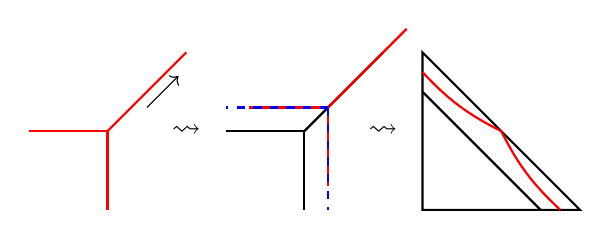
\begin{tikzpicture}[scale=1,transform shape]
    \draw[thick,red] (1,1) -- (0,0);
    \draw[thick,red] (0,-1) -- (0,0);
    \draw[thick,red] (-1,0) -- (0,0);
    \draw[->] (0.5,0.3) -- (0.9,0.7);
    \node (A) at (1,0) {$\rightsquigarrow$};
    \draw[thick] (3.5,1) -- (2.5,0);
    \draw[thick] (2.5,-1) -- (2.5,0);
    \draw[thick] (1.5,0) -- (2.5,0);
    \draw[thick,red] (3.8,1.3) -- (2.8,0.3);
    \draw[thick,red] (2.8,-0.7) -- (2.8,0.3);
    \draw[thick,red] (1.8,0.3) -- (2.8,0.3);
    \node (A2) at (3.5,0) {$\rightsquigarrow$};
    \draw[thick] (4,1) -- (4,-1) -- (6,-1) -- cycle;
    \draw[thick] (5.5,-1) -- (4,0.5);
    \draw[thick,red] (5.75,-1) to [bend left=10] (5,0);
    \draw[thick,red] (4,0.75) to [bend right=10] (5,0);
    \draw[dashed,thick,blue] (2.8,0.3) -- (2.8,-1);
    \draw[dashed,thick,blue] (2.8,0.3) -- (1.5,0.3);
  \end{tikzpicture}
  \caption{Tropical shift}
  \label{fig:trop_shift}
\end{figure}

A more complicated example is shown in~\Cref{fig:trop_shift2}.
\begin{figure}[htpb]
  \centering
  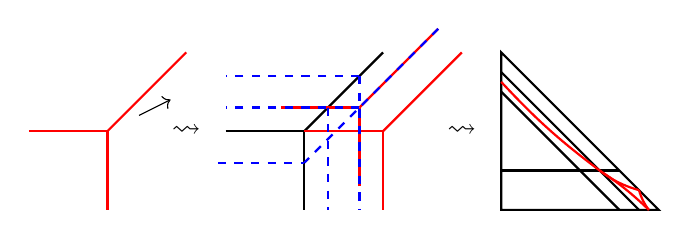
\begin{tikzpicture}[scale=1,transform shape]
    \draw[thick,red] (1,1) -- (0,0);
    \draw[thick,red] (0,-1) -- (0,0);
    \draw[thick,red] (-1,0) -- (0,0);
    \draw[->] (0.4,0.2) -- (0.8,0.4);
    \node (A) at (1,0) {$\rightsquigarrow$};
    \draw[thick] (3.5,1) -- (2.5,0);
    \draw[thick] (2.5,-1) -- (2.5,0);
    \draw[thick] (1.5,0) -- (2.5,0);
    \draw[thick,red] (4.2,1.3) -- (3.2,0.3);
    \draw[thick,red] (3.2,-0.7) -- (3.2,0.3);
    \draw[thick,red] (2.2,0.3) -- (3.2,0.3);
    \draw[thick,red] (4.5,1) -- (3.5,0);
    \draw[thick,red] (2.5,0) -- (3.5,0);
    \draw[thick,red] (3.5,-1) -- (3.5,0);
    \node (A2) at (4.5,0) {$\rightsquigarrow$};
    \draw[dashed,thick,blue] (3.2,0.7) -- (3.2,-1);
    \draw[dashed,thick,blue] (3.2,0.7) -- (1.5,0.7);
    \draw[dashed,thick,blue] (3.2,0.3) -- (1.5,0.3);
    \draw[dashed,thick,blue] (4.2,1.3) -- (2.5,-0.4);
    \draw[dashed,thick,blue] (1.4,-0.4) -- (2.5,-0.4);
    \draw[dashed,thick,blue] (2.8,0.3) -- (2.8,-1);
    \draw[thick] (5,1) -- (5,-1) -- (7,-1) -- cycle;
    \draw[thick] (6.5,-1) -- (5,0.5);
    \draw[thick] (6.75,-1) -- (5,0.75);
    \draw[thick] (5,-0.5) -- (6.5,-0.5);
    \draw[thick,red] (6.875,-1) to [bend left=10] (6.75,-0.75);
    \draw[thick,red] (6.25,-0.5) to [bend right=10] (6.75,-0.75);
    \draw[thick,red] (6.875,-1) to [bend right=5] (6.25,-0.5);
    \draw[thick,red] (6.25,-0.5) to [bend left=5] (5,0.625);
  \end{tikzpicture}
  \caption{More interesting tropical shift}
  \label{fig:trop_shift2}
\end{figure}

The moduli space is simply $\mc{M}(\T^2) = \T^2$, and after the refinement, we obtain that $\mc{M}(\P^2)$ has tropical part the toric fan of $\P^2$ blown up at the three fixed points. The smooth part is simply $\P^2$ blown up at $3$ points, and the moduli space itself is its explosion. As in the case of relative enumerative geometry, the rubber components need to be quotiented out by symmetries in the approaches of Ionel and Tehrani. However, we should note differences in the two approaches, as seen in~\Cref{fig:comparison}.
\begin{figure}[htpb]
  \centering
  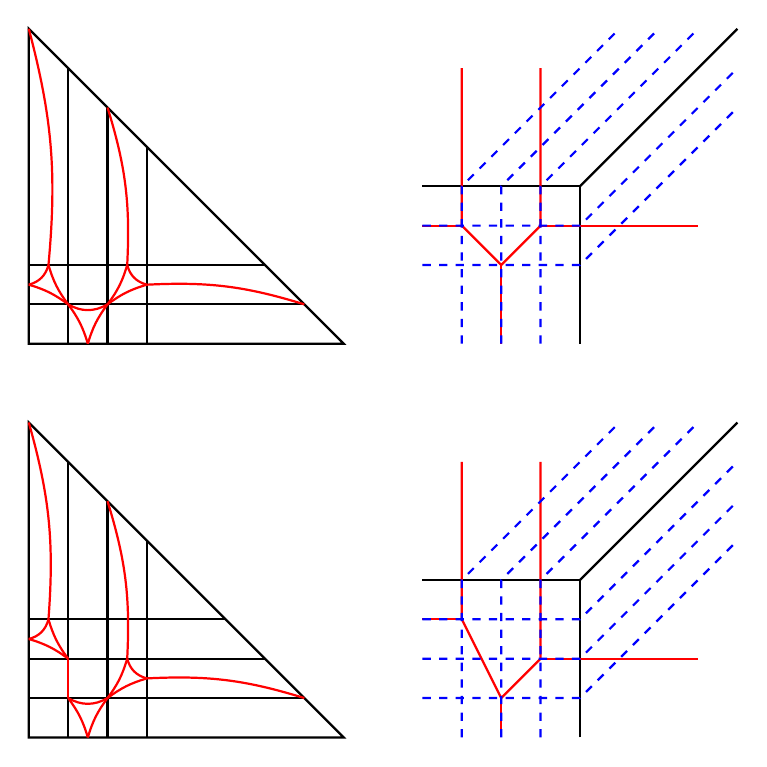
\begin{tikzpicture}[scale=1,transform shape]
    \draw[thick] (0,-2) -- (4,-2) -- (0,2) -- cycle;
    \draw[thick] (0.5,-2) -- (0.5,1.5);
    \draw[thick] (1,-2) -- (1,1);
    \draw[thick] (1.5,-2) -- (1.5,0.5);
    \draw[thick] (0,-1.5) -- (3.5,-1.5);
    \draw[thick] (0,-1) -- (3,-1);
    \draw[red,thick] (0.75,-2) to [bend left=10] (1,-1.5);
    \draw[red,thick] (0.75,-2) to [bend right=10] (0.5,-1.5);
    \draw[red,thick] (0.5,-1.5) to [bend right=30] (1,-1.5);
    \draw[red,thick] (0.5,-1.5) to [bend right=10] (0,-1.25);
    \draw[red,thick] (0.25,-1) to [bend left=30] (0,-1.25);
    \draw[red,thick] (0.5,-1.5) to [bend left=10] (0.25,-1);
    \draw[red,thick] (1,-1.5) to [bend left=10] (1.5,-1.25);
    \draw[red,thick] (1.25,-1) to [bend right=30] (1.5,-1.25);
    \draw[red,thick] (1,-1.5) to [bend right=10] (1.25,-1);
    \draw[red,thick] (0.25,-1) to [bend right=10] (0,2);
    \draw[red,thick] (1.25,-1) to [bend right=10] (1,1);
    \draw[red,thick] (1.5,-1.25) to [bend left=10] (3.5,-1.5);
    \draw[thick] (5,0) -- (7,0);
    \draw[thick] (7,-2) -- (7,0);
    \draw[thick] (7,0) -- (9,2);
    \draw[thick,red] (5.5,1.5) -- (5.5,-0.5) -- (6,-1) -- (6.5,-0.5) -- (6.5,1.5);
    \draw[thick,red] (6,-1) -- (6,-2);
    \draw[thick,red] (6.5,-0.5) -- (8.5,-0.5);
    \draw[thick,red] (5.5,-0.5) -- (5,-0.5);
    \draw[thick,dashed,blue] (5,-1) -- (7,-1) -- (9,1);
    \draw[thick,dashed,blue] (5,-0.5) -- (7,-0.5) -- (9,1.5);
    \draw[thick,dashed,blue] (5.5,-2) -- (5.5,0) -- (7.5,2);
    \draw[thick,dashed,blue] (6,-2) -- (6,0) -- (8,2);
    \draw[thick,dashed,blue] (6.5,-2) -- (6.5,0) -- (8.5,2);
    \draw[thick] (0,-7) -- (4,-7) -- (0,-3) -- cycle;
    \draw[thick] (0.5,-7) -- (0.5,-3.5);
    \draw[thick] (1,-7) -- (1,-4);
    \draw[thick] (1.5,-7) -- (1.5,-4.5);
    \draw[thick] (0,-6.5) -- (3.5,-6.5);
    \draw[thick] (0,-6) -- (3,-6);
    \draw[thick] (0,-5.5) -- (2.5,-5.5);
    \draw[red,thick] (0.75,-7) to [bend left=10] (1,-6.5);
    \draw[red,thick] (0.75,-7) to [bend right=10] (0.5,-6.5);
    \draw[red,thick] (0.5,-6.5) to [bend right=30] (1,-6.5);
    \draw[red,thick] (0.5,-6) to [bend right=10] (0,-5.75);
    \draw[red,thick] (0.25,-5.5) to [bend left=30] (0,-5.75);
    \draw[red,thick] (0.5,-6) to [bend left=10] (0.25,-5.5);
    \draw[red,thick] (1,-6.5) to [bend left=10] (1.5,-6.25);
    \draw[red,thick] (1.25,-6) to [bend right=30] (1.5,-6.25);
    \draw[red,thick] (1,-6.5) to [bend right=10] (1.25,-6);
    \draw[red,thick] (0.25,-5.5) to [bend right=10] (0,-3);
    \draw[red,thick] (1.25,-6) to [bend right=10] (1,-4);
    \draw[red,thick] (1.5,-6.25) to [bend left=10] (3.5,-6.5);
    \draw[red,thick] (0.5,-6.5) -- (0.5,-6);
    \draw[thick] (5,-5) -- (7,-5);
    \draw[thick] (7,-7) -- (7,-5);
    \draw[thick] (7,-5) -- (9,-3);
    \draw[thick,red] (5.5,-3.5) -- (5.5,-5.5) -- (6,-6.5) -- (6.5,-6) -- (6.5,-3.5);
    \draw[thick,red] (6,-6.5) -- (6,-7);
    \draw[thick,red] (6.5,-6) -- (8.5,-6);
    \draw[thick,red] (5.5,-5.5) -- (5,-5.5);
    \draw[thick,dashed,blue] (5,-6) -- (7,-6) -- (9,-4);
    \draw[thick,dashed,blue] (5,-5.5) -- (7,-5.5) -- (9,-3.5);
    \draw[thick,dashed,blue] (5,-6.5) -- (7,-6.5) -- (9,-4.5);
    \draw[thick,dashed,blue] (5.5,-7) -- (5.5,-5) -- (7.5,-3);
    \draw[thick,dashed,blue] (6,-7) -- (6,-5) -- (8,-3);
    \draw[thick,dashed,blue] (6.5,-7) -- (6.5,-5) -- (8.5,-3);
  \end{tikzpicture}
  \caption{Ionel's approach can distinguish between the two situations, Tehrani's cannot.}
  \label{fig:comparison}
\end{figure}
\end{exm}

\section{Computations with Calabi-Yau manifolds}
\label{sec:CY_computations}

We will do another example of a surface, and then we will move on to threefolds. Consider $X = \Bl_{(0,1)} (\P^1 \times \P^1)$ with the strict transform of the toric divisor. Our goal is to compute the number $n_d$ of degree $d$ covers of the exceptional divisor $E$. The blowup modifies our integral affine structure by introducing a cut as in~\Cref{fig:cut}.
\begin{figure}[htpb]
  \centering
  \begin{tikzpicture}[scale=1,transform shape]
    \draw[thick] (0,-1) -- (0,1);
    \draw[thick] (-1,0) -- (1,0);
    \draw[->] (-1,-0.2) -- (-1,0) -- (-0.8,0.2);
    \node (C) at (-1.5,0) {cut};
  \end{tikzpicture}
  \caption{Cut}
  \label{fig:cut}
\end{figure}

We can compute $n_1$ by using the gluing formula for a tropical invariant as in~\Cref{fig:n1}:
\begin{figure}[htpb]
  \centering
  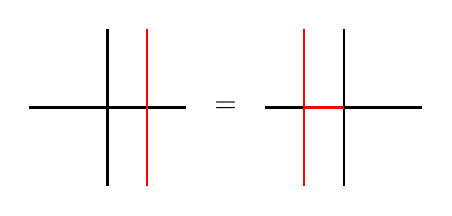
\begin{tikzpicture}[scale=1,transform shape]
    \draw[thick] (0,-1) -- (0,1);
    \draw[thick] (-1,0) -- (1,0);
    \node (E) at (1.5,0) {$=$};
    \draw[thick] (3,-1) -- (3,1);
    \draw[thick] (2,0) -- (4,0);
    \draw[red, thick] (0.5,-1) -- (0.5,1);
    \draw[red, thick] (2.5,-1) -- (2.5,1);
    \draw[red, thick] (2.5,0) -- (3,0);
  \end{tikzpicture}
  \caption{Computing $n_1$}
  \label{fig:n1}
\end{figure}
We then see that $1 = 1 \times n_1$, so $n_1 = 1$.

To compute $n_d$, we obtain the picture in~\Cref{fig:nd}, which gives us
\[ \sum_{\abs{\lambda} = k} \frac{\prod \lambda_i n_{\lambda_i}}{\Aut \lambda} = 0. \]
\begin{figure}[htpb]
  \centering
  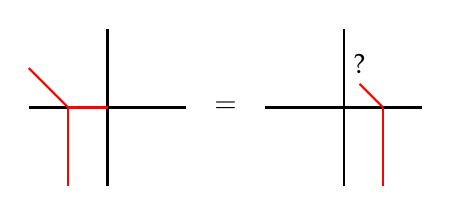
\begin{tikzpicture}[scale=1,transform shape]
    \draw[thick] (0,-1) -- (0,1);
    \draw[thick] (-1,0) -- (1,0);
    \node (E) at (1.5,0) {$=$};
    \draw[thick] (3,-1) -- (3,1);
    \draw[thick] (2,0) -- (4,0);
    \draw[red, thick] (-1,0.5) -- (-0.5,0);
    \draw[red, thick] (-0.5,0) -- (-0.5,-1);
    \draw[red, thick] (-0.5,0) -- (0,0);
    \draw[red, thick] (3.5,-1) -- (3.5,0);
    \draw[red, thick] (3.5,0) -- (3.2,0.3);
    \node[anchor=south] (Q) at (3.2,0.3) {$?$};
  \end{tikzpicture}
  \caption{Computing $n_d$}
  \label{fig:nd}
\end{figure}
If you are a combinatorialist, it is easy to obtain
\[ n_d = \frac{(-1)^{d+1}}{d^2}. \]

We will now consider some threefold examples. Let $B$ be a Calabi-Yau 3-exploded manifold. Then $\ul{B}$ is a $3$-dimensional integral affine manifold with codimension $2$ singular locus $\Gamma$. In some sense, we generically expect that $\Gamma$ has
\begin{itemize}
\item Edges (span a wall coming out of the edge where holomorphic curves can go);
\item Framing changes (where the edge changes the direction by the wall does not);
\item Positive vertices where three edges meet with the sum of their normal directions is $0$;
\item Negative vertices whose normal directions are all the same.
\end{itemize}
In principle, we can compute invariants for all of these local models, but this is actually very difficult.

The nonsingular case is simply $\T^3$. There are inward arrows $v, w, -v-w$ and we obtain (via a quantum deformation)
\[ [\mc{M}_{[\gamma],n}]^{\mr{vir}} = \sum_g [\mc{M}_{[\gamma],g,n}]^{\mr{vir}} \hslash^{2g-2+n}. \]
We then obtain
\[ [\mc{M}_{[\gamma]}]^{\mr{vir}} = [\T^3] \frac{[n]_q}{n}, \qquad [n]_q = \frac{q^{\frac{n}{2}} - q^{\frac{-n}{2}}}{i}, \]
where $q^{\frac{1}{2}} = e^{\frac{i\hslash}{2}}$. 

We will now consider $\ms{Expl}(X, D) \times \T$ (the edge). In fact the picture in~\Cref{fig:n1} is still valid, but instead we obtain $1 = [1]_q \times n_1$, so $n_1 = \frac{1}{[1]_q}$. To compute $n_d$, we have the formula
\[ \sum_{\abs{\lambda} = k} \frac{\prod [ \lambda_i ]_q n_{\lambda_i}}{\Aut \lambda} = 0, \]
which yields us
\[ n_d = \frac{(-1)^{d+1}}{d[d]_q}. \]

We will now consider the case of curves lying on a wall. For each edge on the singular locus, we need to glue over $\ms{Expl}(X, D)$. Fortunately gluing constrained to the wall factors through intersection with $E$, so we obtain a Fock space $H_{\ell}$ associated with the edge.

In any situation as in~\Cref{fig:operator}, we obtain an operator $W_{v, \ell} \colon H_{\ell} \to H_{\ell}$. These satisfy the commutation relation
\[ [ W_{v,\ell}, W_{w, \ell} ] = [v \wedge w]_{q} W_{v+w, \ell} + c_{\ell}(v) \delta_{-v,w}. \]
These are the relations for the quantum torus $W_{1,\infty}$.
\begin{figure}[htpb]
  \centering
  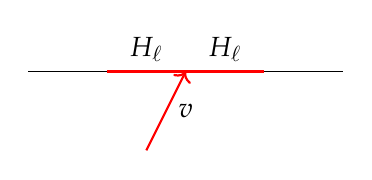
\begin{tikzpicture}[scale=1, transform shape]
    \draw (-2,0) -- (2,0);
    \draw[thick,red] (-1,0) -- (1,0);
    \draw[thick,red,->] (-0.5,-1) -- (0,0);
    \node (v) at (0,-0.5) {$v$};
    \node[anchor=south] (h1) at (-0.5,0) {$H_{\ell}$};
    \node[anchor=south] (h2) at (0.5,0) {$H_{\ell}$};
  \end{tikzpicture}
  \caption{Obtaining an operator}
  \label{fig:operator}
\end{figure}

Performing another tropical computation as in~\Cref{fig:wall}, we obtain the formula
\[ W_{v, \ell} \circ W_{w,\ell} = W_{w,\ell} \circ W_{v,\ell} + [v \wedge w]_q W_{v+w,\ell}. \]
\begin{figure}[htpb]
  \centering
  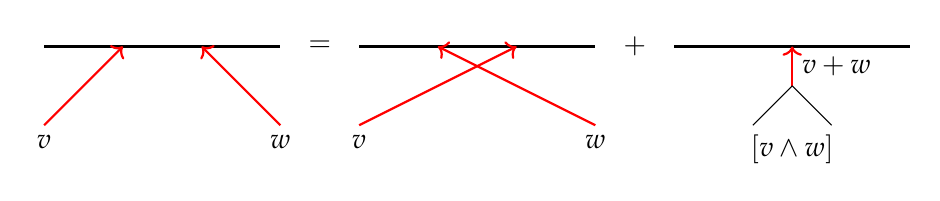
\begin{tikzpicture}[scale=1,transform shape]
    \draw[thick] (0,0) -- (3,0);
    \draw[thick,red,->] (0,-1) -- (1,0);
    \node[anchor=north] (v1) at (0,-1) {$v$};
    \draw[thick,red,->] (3,-1) -- (2,0);
    \node[anchor=north] (w1) at (3,-1) {$w$};
    \node (E) at (3.5,0) {$=$};
    \draw[thick] (4,0) -- (7,0);
    \draw[thick,red,->] (4,-1) -- (6,0);
    \node[anchor=north] (v2) at (4,-1) {$v$};
    \draw[thick,red,->] (7,-1) -- (5,0);
    \node[anchor=north] (w2) at (7,-1) {$w$};
    \node (P) at (7.5,0) {$+$};
    \draw[thick] (8,0) -- (11,0);
    \draw[thick,red,->] (9.5,-0.5) -- (9.5,0);
    \node[anchor=west] (vw) at (9.5,-0.25) {$v+w$};
    \draw (9,-1) -- (9.5,-0.5);
    \draw (10,-1) -- (9.5,-0.5);
    \node[anchor=north] at (9.5,-1) {$[v \wedge w]$};
  \end{tikzpicture}
  \caption{On the wall}
  \label{fig:wall}
\end{figure}


Moving on to the framing change, let the legs be $\ell_1$ and $\ell_2$. The framing change is a map
\[ F \colon \mc{H}_{\ell_1} \to \mc{H}_{\ell_2} \]
which is in fact an isomorphism of representations of $W_{1, \infty}$. To show this, we consider the tropical picture in~\Cref{fig:framing}.
\begin{figure}[htpb]
  \centering
  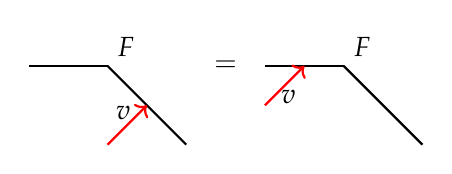
\begin{tikzpicture}[scale=1,transform shape]
    \node[anchor=south west] (F1) at (0,0) {$F$};
    \draw[thick] (-1,0) -- (0,0);
    \draw[thick] (0,0) -- (1,-1);
    \draw[->,thick,red] (0,-1) -- (0.5,-0.5);
    \node (C1) at (0.2,-0.6) {$v$};
    \node (E) at (1.5,0) {$=$};
    \node[anchor=south west] (F2) at (3,0) {$F$};
    \draw[thick] (2,0) -- (3,0);
    \draw[thick] (3,0) -- (4,-1);
    \draw[->,thick,red] (2,-0.5) -- (2.5,0);
    \node (C1) at (2.3,-0.4) {$v$};
  \end{tikzpicture}
  \caption{Framing change}
  \label{fig:framing}
\end{figure}


Now we consider the positive vertex. We will have $\ell_1, \ell_2$ pointing inward and $\ell_3$ pointing out. The vertex will be an intertwiner
\[ T \colon H_{\ell_1} \otimes H_{\ell_2} \to H_{\ell_3} \]
of representations of the quantum torus. The pictures are as in~\Cref{fig:posvert}.

\begin{figure}[htpb]
  \centering
  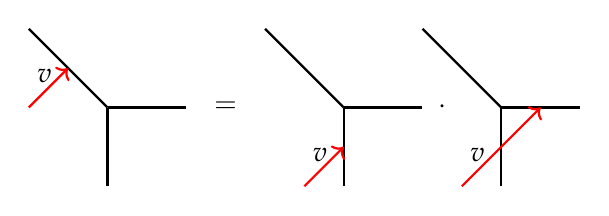
\begin{tikzpicture}[scale=1,transform shape]
    \draw[thick] (-1,1) -- (0,0);
    \draw[thick] (0,-1) -- (0,0);
    \draw[thick] (1,0) -- (0,0);
    \draw[->,thick,red] (-1,0) -- (-0.5,0.5);
    \node (C1) at (-0.8,0.4) {$v$};
    \node (E) at (1.5,0) {$=$};
    \draw[thick] (2,1) -- (3,0);
    \draw[thick] (3,-1) -- (3,0);
    \draw[thick] (4,0) -- (3,0);
    \draw[->,thick,red] (2.5,-1) -- (3,-0.5);
    \node (C2) at (2.7,-0.6) {$v$};
    \draw[thick] (4,1) -- (5,0);
    \draw[thick] (5,-1) -- (5,0);
    \draw[thick] (6,0) -- (5,0);
    \draw[->,thick,red] (4.5,-1) -- (5.5,0);
    \node (C3) at (4.7,-0.6) {$v$};
    \node (D) at (4.25,0) {$\cdot$};
  \end{tikzpicture}
  \caption{Positive vertex}
  \label{fig:posvert}
\end{figure}

In the case of the negative vertex (point all edges inwards), the operator $N$ diagonalizes as
\[ N = \sum_{\lambda} c^{\abs{\lambda}} q^{c(\lambda)} \prod_{\square \in \lambda} [h \square]_q \ul{\lambda} \otimes \ul{\lambda} \otimes \ul{\lambda}. \]
There is a nice interpretation of this due to Bryan-Pandharipande in terms of representations of the symmetric group as usual.

\chapter{Logarithmic and punctured Gromov-Witten invariants, tropicalization, and gluing formalism (Bernd Siebert)}%

\section{Introduction to log geometry}

We will be relatively liberal in the category we work in. We may consider either algebraic varieties or complex manifolds/analytic spaces. These get generalized to algebraic stacks (or analytic stacks), which we will consider later.

\subsection{Normal crossings divisors}

Let $X$ be smooth and $D \subseteq X$ be a divisor such that locally, $D = V(z_1 \cdots z_k)$, where $z_1, \ldots, z_n$ are local coordinates. This is really bad for algebraic geometry. Instead, we may consider

\begin{defn}
    A \textit{simple normal crossings} divisor is such that there exists $U \subseteq X$ open and a smooth $\pi \colon U \to \A^r$ such that $D \cap U = \pi^{-1}(V(z_1 \cdots z_r))$.
\end{defn}

All such $D$ can be written as $D = \bigcup D_i$, where the $D_i \subseteq X$ are smooth divisors intersecting transversely. In general, we need an \'etale $U \to X$ such that the preimage of $D$ is a simple normal crossings divisor.

For a simple normal crossings divisor $D = \bigcup D_i$, we obtain line bundles $L_i$ with sections $s_i$ and corresponding sheaves $\mc{L}_i = \mc{O}_X(D_i)$. Every section $s_i$ is a map $\mc{O}_X \to \mc{O}_X(D_i)$, or equivalently, a map $\mc{O}_X(-D_i) \to \mc{O}_X$. In addition, the normal bundles of $D_i \subseteq X$ is
\[ \mc{N}_{D_i/X} = \mc{O}_{D_i}(D_i) = \mc{L}_i |_{D_i}. \]

Iterating, we see that $D_i \cap D \subseteq D_j$ is a simple normal crossings in $D_i$ with normal bundle
\[ \mc{N}_{D_i \cap D_j/X} = \mc{N}_{D_i \cap D_j / D_i} \oplus \mc{N}_{D_i/X}. \]
All of this is contained in $\mc{M}_X \coloneqq \mc{O}_{X/D}^{\times} \cap \mc{O}_X \hookrightarrow \mc{O}_X$. Unfortunately, this is a sheaf of multiplicative monoids and has no additional structure.

\begin{exm}
    Consider $\A^2_{z,w}$ with $D = V(zw)$. If we consider the sheaf $\mc{M}_X$, away from $D$ we see all $h \in \mc{O}^{\times}$, on the $z$-axis we have $h \cdot w^b, h \in \mc{O}^{\times}$, and at the origin we see $h \cdot z^a w^b$. As a monoid, we have
    \[ \mc{M}_{X,0} \simeq \N^2 \times \mc{O}_{X,0}^{\times}. \]
\end{exm}

We can then take the associated abelian sheaf $\mc{M}_X^{\mr{gp}}$, which replaces the $\N$-factors by $\Z$-factors. This has a discrete part $\ol{\mc{M}}_X = \mc{M}_X/\mc{O}_X^{\times}$ with quotient map $\kappa$. In general, in the simple normal crossings case, we have
\[ \ol{\mc{M}}_X = \bigoplus_i \N_{D_i}. \]
We may recover the line bundles in the simple normal crossings case. Taking the groupification, we obtain
\[ 1 \to \mc{O}_X^{\times} \to \mc{M}_X^{\mr{gp}} \to \ol{\mc{M}}_X^{\mr{gp}} \to 0, \]
and thus $\mc{M}_X^{\mr{gp}}$ is a $\mc{O}_X^{\times}$-torsor. Considering $\mc{T} \coloneqq \kappa^{-1}((a_1, \ldots, a_r))$, we can brute force the sheaf
\[ (\mc{T} \oplus \mc{O}_X) / \mc{O}_X^{\times} = \mc{O}_X\qty(-\sum a_i D_i). \]

\subsection{Toric geometries}

Consider a finitely generated submonoid $P \subseteq (\Z^n, +)$. Explicitly, we can write $P = \N m_1 + \cdots + \N m_r$. The most imporant case is when we take $\sigma^{\vee} \cap \Z^n$, where $\sigma \subseteq (\R^n)^*$ is a rational polyhedral cone. It is customary to write $(\R^n)^* \simeq N \otimes \R$ and $P \subseteq M$ for the two different $\Z^n$.

Using $P$, we obtain a finitely-generated $\C$-algebra $\C[P] = \qty{\sum_{m \in P} a_m z^m}$, where the sums are finite. Explicitly, we can consider the map
\[ \varphi \colon \C[u_1, \ldots, u_r] \twoheadrightarrow \C[P] \qquad u_i \mapsto z^{m_i}, \]
which give equations for the ring. The relations always come from relations in $P$, so $\ker \varphi$ is generated by binomial equations $z^{m_1} z^{m_2} = z^{m_1'} z^{m_2'}$ (in the saturated case). Applying the $\Spec$ functor, we obtain
\[ \Spec \C[P] \hookrightarrow \A^r. \]

In fact, we always have $P \subseteq \sigma^{\vee} \cap M$ with $\sigma = \Hom(P, \R_{\geq 0})$ with equality if and only if $P$ is saturated.

\begin{exm}
    Consider $P \subseteq \N \cdot 2 + \N \cdot 3 \subseteq \Z = M$. Then $\C[P] = \C[x,y]/(x^3-y^2)$.
\end{exm}

\begin{exms}\leavevmode
    \begin{enumerate}[(a)]
        \item Consider the cone generated by $(0,1)$ and $(k,1)$ in $N_{\R}$. Then the dual cone is generated by $(-1,k)$ and $(1,0)$ over $\R$, and the monoid $P = \sigma^{\vee} \cap M$ is generated by $(1,0), (0,1)$, and $(-1, k)$. Writing the corresponding variables as $z,w,t$, we obtain
            \[ C[P] = \C[z,w,t]/(zw-t^k), \]
            which is the $A_{k-1}$ singularity. Note that this is the base change under $t \mapsto t^k$ of the normal crossings degeneration $(zw-t)$.
        \item Let $\sigma^{\vee}$ be the cone over the convex hull of the square $\qty{(0,0), (1,0), (1,1), (0,1)}$. Then 
            \[ \C[\sigma^{\vee} \cap M] \simeq \C[x,y,z,w] / (xy-zw) \]
            is a tensor product
            \[ \C[x,y] \otimes_{\C[t]} \C[z,w] \qquad xy \mapsfrom t \mapsto zw. \]
    \end{enumerate}
\end{exms}

Because we have $P = \sigma^{\vee} \cap M$, we obtain $\C[P] \subseteq \C[M]$. This gives us an $M$-grading, which induces a $(\C^{\times})^n$-equivariant embedding
\[ (\C^{\times})^n = \Spec \C[M] \hookrightarrow \Spec \C[P] = X_{\sigma}. \]

\begin{defn}
    A \textit{toric variety} is a $(\C^{\times})^n$-equivariant partial compactification of $(\C^{\times})^n$.
\end{defn}

\begin{rmk}
    We will want $P$ to be saturated, which corresponds to the toric variety being normal.
\end{rmk}

\begin{defn}
    The \textit{toric divisor} is the complement $x_{\sigma} \setminus (\C^{\times})^n$, and its components $D_i$ can be read off from the facets of $P$ (or $P_{\R} = \R_{\geq 0} \cdot P$).
\end{defn}

An alternative construction of toric varieties is as follows. Consider $N \simeq \Z^n$. Then let $\sigma(1)$ be the set of rays, labelled $\rho_1, \ldots, \rho_r$. Then we define the \textit{Cox ring} to be
\[ R \coloneqq \C[\on{Map}(\sigma(1), \N)] = \C[\chi_1, \ldots, \chi_r]. \]
Then there is a map $M \to \on{Map}(\sigma(1), \Z)$ given by $m \mapsto (\rho_i \mapsto \ev{m, n_i})$, where $n_i$ is the primitive generator of $\rho_i$. Grading $R$ by $\Gamma = \on{Map}(\sigma(1), \Z)/M$, we obtain an action of $(\C^{\times})^{r-n}$-action on $R$. Taking the categorical quotient $\Spec R^{\Gamma}$, we obtain $X_{\sigma}$.

\begin{exer}
    Show that $R^{\Gamma} = \C[P]$ where $P = \sigma^{\vee} \cap M$.
\end{exer}

The upshot is that an affine toric variety can be written as $\Spec \C[P] = \A^r \sslash_0 (\C^{\times})^{r-n}$.

In this case, if $X = X_{\sigma}$, then generalizing $\mc{M}_{\A^n} = \mc{O}_{\A^n \setminus V(z_1\cdots z_n)} \cap \mc{O}_{\A^n} \hookrightarrow \mc{O}_{\A^n}$, we can write
\[ \mc{M}_X \coloneqq \mc{O}_{X\setminus D}^{\times} \hookrightarrow \mc{O}_X. \]
As long as $0$ is the only invertible element of $P$, we have
\[ \ol{\mc{M}}_{X,0} = P. \]
Now we have an embedding
\[ \Gamma(\ol{\mc{M}}_{X}^{\mr{gp}}) \hookrightarrow \Z^r \qquad f \mapsto (\on{ord}_{D_1} f, \ldots, \on{ord}_{D_r} f). \]
The image corresponds to principal Cartier divisors.

\begin{exm}
    If $\sigma$ is the cone over the square, then $D = \sum a_i D_i$ is Cartier if and only if $a_1+a_3 = a_2 + a_4$.
\end{exm}

\subsection{Abstract log structures}
Consider $\alpha \colon \mc{M}_X \to \mc{O}_X$ in the \'etale topology such that $\alpha^{-1}(\mc{O}_X^{\times}) \xrightarrow[\alpha]{\simeq} \mc{O}_X^{\times}$. This definition is useless in this generality, but it does automatically provide us with
\[ \ol{\mc{M}}_X, \mc{M}_X^{\mr{gp}}, \kappa \]
as before.

We will instead provide an alternative point of view, due to Deligne-Faltings. We want the following data:
\begin{itemize}
    \item A sheaf of finitely generated $\ol{\mc{M}}$ inside $\ol{\mc{M}}_X^{\mr{gp}}$ constructible;
    \item For all $U \subseteq X$, a map 
        \[ \ol{\mc{M}}(U) \to \on{\mc{D}iv}(U) = \qty{(\text{line bundle, section}) \text{ on }U} \qquad \ol{m} \mapsto (\alpha_{\ol{m}} \colon \kappa^{-1}(\ol{m}) \to \mc{O}_X)^{\vee}. \]
    \item We have compatibility $\ol{\mc{M}} \to \on{\mc{D}iv}_X$ which is morally a symmetric monoidal functor.%\footnote{The reference with the answers is {\href{this paper}{https://www.sciencedirect.com/science/article/pii/S0001870812002368}} by Borne-Vistoli}
\end{itemize}

\begin{exms}\leavevmode
    \begin{enumerate}[(a)]
        \item Consider \textit{log points}, which are given by $\Spec(Q \to \C) = (\Spec \C, Q \oplus \C^{\times})$. Here, we need $Q$ a finitely generated monoid with $Q^{\times} = \qty{0}$, and we have
            \[ \alpha(q,a) = \begin{cases}
                0 & q \neq 0 \\
                a & q = 0.
            \end{cases}
            \]
        \item We can consider \textit{pullback log structures} for morphisms $f \colon Y \to X$ with a log structure $\mc{M}_X$ on $X$. We obtain a log structure on $Y$ by writing
            \[ f^* \mc{M}_X = (f^{-1} \mc{M}_X \oplus \mc{O}_Y^{\times}) / f^{-1} \mc{O}_X^{\times} \]
            and send $(s,h) \mapsto f^*\alpha(s) \cdot h$.
    \end{enumerate}
\end{exms}

Note that if $Q = \sigma^{\vee} \cap M$ and $0 \hookrightarrow X_{\sigma}$ is the inclusion of a $0$-dimensional orbit, the pullback log structure is $f^* \mc{M}_{X_{\sigma}} = \Spec(Q \to \C)$.

An important class of examples are those with charts. Consider an open set $U \subseteq X$ (maybe in the \'etale topology) and a map $f \colon U \to \Spec \C[P]$, where $P$ is as in the previous subsection, with isomorphisms $\mc{M}_X|_U \simeq f^* \mc{M}_{\Spec \C[P]}$. The \textit{fine log structures} are those with local charts and a \textit{fine saturated log structure} is one with $P$ saturated.

\begin{defn}
    A \textit{log morphism} $f \colon (X, \mc{M}_X) \to (Y, \mc{M}_Y)$ is a map $f \colon X \to Y$ (which gives us $f^{\sharp} \colon f^{-1}\mc{O}_Y \to \mc{O}_X)$ and a morphism of sheaves $f^{\flat} \colon f^{-1} \mc{M}_Y \to \mc{M_X}$ making the diagram
    \begin{equation*}
    \begin{tikzcd}
        f^{-1}\mc{M}_Y \ar{r}{f^{\flat}} \ar[swap]{d}{f^{-1}\alpha_Y} & \mc{M}_X \ar{d}{\alpha_X} \\
        f^{-1} \mc{O}_Y \ar{r}{f^{\sharp}} & \mc{O}_X
    \end{tikzcd}
    \end{equation*}
    commute.
\end{defn}

We will refer to $\ol{\mc{M}}$ as the \textit{ghost sheaf}. Others call it the \textit{characteristic sheaf}, but Bernd prefers to call it the ghost sheaf.

\subsection{Log smooth morphisms}
\label{subsec:log_smooth}

These morphisms are locally given by toric morphisms. Suppose we have a morphism $Q \to P$ of monoids. Then we require the existence of a diagram
\begin{equation*}
  \begin{tikzcd}
    X \ar{r}{\text{smooth}} \ar{dr}{f} & Y \times_{A_Q} A_P \ar{r}{\varphi} \ar{d} & \Spec \C[P] = A_P \ar{d} \\
    & Y \ar{r} & \Spec \C[Q]
  \end{tikzcd}
\end{equation*}

\begin{exm}
  The basic example is the diagram
\begin{equation*}
  \begin{tikzcd}
    X \ar{r} \ar{dr}{f} & Y \times_{\A^1} \A^r \ar{r}{\varphi} \ar{d} & \A^r\ar{d}{\prod z_i} \\
    & Y \ar{r} & \A^1
  \end{tikzcd}
\end{equation*}
\end{exm}

\begin{exms}\leavevmode
\begin{enumerate}[(a)]
\item We can allow $Q = 0$. Then we require the existence of a divisor $D \subseteq X$ such that $(X, D)$ is a toroidal pair.
\item If we consider $Q = \N$ and $P = \N^r$ with the map $1 \mapsto (1, \ldots, 1)$, these are base changes of normal crossings degenerations.
\item Let $0^{\dag} = \Spec (\N \to \C)$ be the standard log point. Then if $Y$ is a curve, the central fiber
  \begin{equation*}
    \begin{tikzcd}
      X_0 \ar[hookrightarrow]{r} \ar{d} & X \ar{d} \\
      0^{\dag} \ar[hookrightarrow]{r} & Y
    \end{tikzcd}
  \end{equation*}
  is a normal crossings degeneration.
\item Let $f \in \C[z_0, \ldots, z_3]$ be homogeneous of degree $4$. Define
  \[ X' = V(tf(z_1, \ldots, z_3) + z_0 \cdots z_3) \subseteq \A^1_t \times \P^3_{z_0 \ldots z_3}. \]
  This is singular, where the singular locus $(X_0')_{\mr{sing}} \cap V(f)$ consists of $24$ $A_1$ singularities. If we consider $X_0' \subseteq X'$, this is a very bad at the singularities, meaning they are not fine. To resolve this, we can simply blow up the singularities in some order to obtain a smooth total space $X$ which is a normal crossings degeneration and hence log smooth.

  Suppose we have a normal crossings degeneration $X_0 \subseteq X$. Then this $X_0$ is $d$-semistable in the sense of Friedman. What this means is that
  \[ \on{\mc{E}xt}^1(\Omega^1_{X_0}) \in \Pic((X_0)_{\mr{sing}}) \]
  is a trivial bundle. He proved that a $d$-semistable K3 surface is smoothable. In higher dimension, this is very tricky.

  This story can be reinterpreted in terms of log geometry following Kawamata and Namikawa. They showed that a normal crossings variety $X_0$ is $d$-semistable if and only if there exists a log structure $\mc{M}_{X_0}$ and a log smooth morphism
  \[ (X_0, \mc{M}_{X_0}) \to \Spec (\N \to \C). \]

  All of this has a symplectic analogue due to McLean-Tehrani-Zinger, which states that symplectically $d$-semistable implies symplectically smoothable.
\end{enumerate}
\end{exms}

\subsection{Kato-Nakayama spaces}
\label{subsec:knspace}

For any $(X, \mc{M}_X)$, this is a topological space $(X, \mc{M}_X)^{\mr{KN}} \to X$ which provides a ``topological smoothing'', where if we have a diagram
\begin{equation*}
  \begin{tikzcd}
    X_0 \ar[hookrightarrow]{r} \ar{d} & X \ar{d}{\pi} \\
    \Spec(\N \to \C) \ar[hookrightarrow]{r} & S,
  \end{tikzcd}
\end{equation*}
then the KN functor will give us a map $X_0^{\mr{KN}} \to S^1$ which should be thought of as a restriction of $\pi$ to the locus lying over a small circle.

\section{Tropicalization}
\label{sec:tropicalization}

Traditionally, we would begin with a valued $\C$-algebra, for example
\[ K = \C \{\{t\}\} = \bigcup_{k > 0} \C((t^{1/k}). \]
If we choose an ideal $I \subseteq K[z_1^{\pm}, \ldots z_n^{\pm}]$, we obtain an algebraic subvariety $V(I) \subseteq (K^{\times})^n$. Applying the valuation
\[ \on{val} \colon (K^{\times})^n \to \R^n, \]
we can define the \textit{tropicalization} in various ways:
\begin{align*}
\ms{Trop}(X) &= \ol{\on{val}(V(I))} \\
             &= \qty{w \in \R^n \mid \on{in}_w(I) \neq (1)} \\
             &= V(\ms{trop}(I)),
\end{align*}
where $\ms{trop}(I) \subseteq (\R, \max, +)[x_1^{\pm}, \ldots, x_n^{\pm}]$ is the tropicalization of $I$.

If we have convergent Puiseux series, we can consider $(X_t)_{t \neq 0} \subseteq (\C^{\times})^n$, and then take
\[ \log_t(X_t) \xrightarrow{t \to 0} \ms{Trop}(X). \]

\subsection{Tropicalization in log geometry}
\label{subsec:trop_log}

Consider a fine log space $X = (\ul{X}, \ms{M}_X)$. For all $x \in X$, we will write $P_x = \ol{\mc{M}}_{X,x}$. This is a finitely generated monoid with $P_x^{\times} = \qty{0}$. In algebraic geometry, if $y \in X$ is a non-closed point and $x$ is a specialization of $Y$, then there is a \textit{generization map}
\[ P_x \twoheadrightarrow P_y = (P_x + F^{\mr{gp}})/ F^{\mr{gp}}. \]
Here, $F \subseteq P_x$ is a face $\qty{p \mid \alpha(p) \in \mc{O}_{X,y}^{\times}}$.

In the analytic world, we can instead find an open set $U$ around $x$ such that $\ol{\mc{M}}_X(U) \to \ol{\mc{M}}_{X,x} = P_x$ is an isomorphism. Then, we have a diagram
\begin{equation*}
  \begin{tikzcd}
    \ol{\mc{M}}_X(U) \ar{r}{\simeq} \ar[twoheadrightarrow]{dr} & P_X \ar[dashrightarrow]{d} \\
    & P_Y
  \end{tikzcd}
\end{equation*}
defining the generization map.

Dualizing, consider the rational polyhedral cone $\sigma_x = \Hom(P_x, (\R_{\geq 0}, +))$. Because we have the surjective generization map which is projection along a face $F$, we have
\[ \sigma_y \xrightarrow{\simeq} \sigma_X \cap F^{\perp} \hookrightarrow \sigma_x. \]
In the case of $\P^1 \times \P^1$, we can recover the correspondence between orbits and the fan, and finally we set
\[ \on{\ms{Trop} X} \coloneqq \varinjlim_{x \in X} \sigma_x. \]

\begin{prop}
If $X$ is the toric variety corresponding to a fan $\Sigma$, then $\on{\ms{Trop}} X = \Sigma$ with the embedding into $N_{\R}$ forgotten.
\end{prop}

\begin{warn}
  It should be noted that if $X = \Bl_1(\P^1 \times \P^1)$ and $D = \bigcup_4 \P^1$, then
  \[ \on{\ms{Trop}} X = \on{\ms{Trop}} \P^1 \times \P^1. \]
  In fact, if we take any toric surface with four boundary divisors (for example a Hirzebruch surface), we obtain the same tropicalization. This is in fact a \textbf{feature} of the theory.
\end{warn}

\begin{exm}[Whitney umbrella]
  Consider coordinates $x,y,z$ on $\A^3$ and consider $\wt{D} = V(xy)$. Consider the $\Z/2\Z$ action given by
  \[ (x,y,z) \mapsto (y,x,-z). \]
  Taking the quotient, we obtain
  \[ \wt{D} / (\Z/2\Z) \simeq V(uv^2-w^2) \subseteq \A^3. \]
  Removing the origin, we can set $X = \A^3 \setminus \qty{0}$ with divisor $\wt{D}/(\Z/2\Z)$. If we consider $\wt{\ell}$ to be the $z$-axis, we note that
  \[ \mc{M}_(\A^3, \wt{D})|_{\ell} = \ul{\N^2}, \]
  so $\mc{M}_{X}|_{\ell}$ is locally constant (it sees the monodromy of swapping $x$ and $y$). Finally, we get that $\on{\ms{Trop}}(X)$ is the generalized cone complex (locally a limit of cone complexes) shown in~\Cref{fig:whitney}.
  \begin{figure}[htpb]
    \centering
    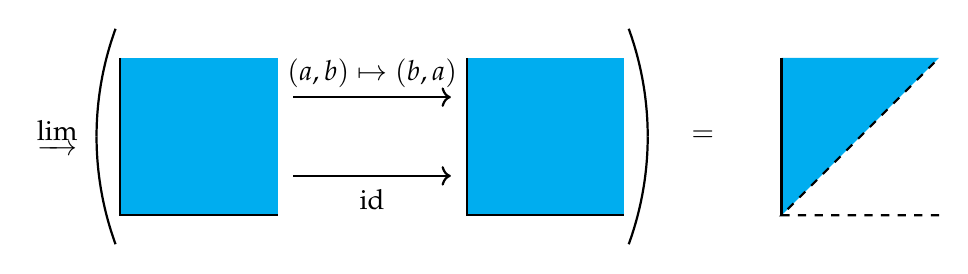
\begin{tikzpicture}[scale=1, transform shape]
      \node (L) at (0,0) {$\varinjlim$};
      \fill[fill=cyan] (0.8,-1) rectangle (2.8,1);
      \fill[fill=cyan] (5.2,-1) rectangle (7.2,1);
      \draw[thick] (0.8,1) -- (0.8,-1) -- (2.8,-1);
      \draw[thick] (5.2,1) -- (5.2,-1) -- (7.2,-1);
      \draw[thick,->] (3,0.5) -- (5,0.5);
      \draw[thick,->] (3,-0.5) -- (5,-0.5);
      \node (I) at (4, -0.8) {$\mr{id}$};
      \node (S) at (4, 0.8) {$(a,b) \mapsto (b,a)$};
      \fill[fill=cyan] (9.2,1) -- (9.2,-1) -- (11.2,1) -- cycle;
      \draw[thick] (9.2,1) -- (9.2, -1);
      \draw[thick,dashed] (11.2,-1) -- (9.2,-1) -- (11.2, 1);
      \node (E) at (8.2, 0) {$=$};
      \draw[thick] (0.5,0) arc[start angle=180, end angle=160,radius=4];
      \draw[thick] (0.5,0) arc[start angle=180, end angle=200,radius=4];
      \draw[thick] (7.5,0) arc[start angle=0, end angle=-20,radius=4];
      \draw[thick] (7.5,0) arc[start angle=0, end angle=20,radius=4];
    \end{tikzpicture}
    \caption{Tropicalization of the Whitney umbrella}
    \label{fig:whitney}
  \end{figure}
\end{exm}

\section{Log smooth curves}
\label{sec:log_smooth_curves}

These are simply normal crossings degenerations of smooth curves with marked points. These will be domains for stable log maps, which will define logarithmic Gromov-Witten theory. There are three types of local models for $\mc{M}_C |_{C_0}$. Let $z$ be the fiber direction and $t$ be the base direction.
\begin{itemize}
\item At the generic points $\eta$ of $C_0$, the map is given by $(z,t) \mapsto t$, so
  \[ \ol{\mc{M}}_{C_0, \eta} = \N = \ev{t}. \]
\item At a marked point $p$ of $C_0$, we can see both the base and fiber directions, so we obtain
  \[ \ol{\mc{M}}_{C_0, p} = \N \oplus \N = \ev{z,t}. \]
  Here, this receives a map from $\N$ going into the first factor.
\item At a node $q$, we have $(z,w) \mapsto zw = t$, and thus
  \[ \ol{\mc{M}}_{C_0, q} = \N^2 = \ev{z,w}. \]
  This receives a map from $\N$ where $1 \mapsto (1,1)$.
\end{itemize}

Generally, we want to consider curves $C \to \Spec(\N \to \C)$ which are log smooth, integral, have $\ul{C}$ reduced, have fine separated log structures, and are of relative dimension $1$. In this case, $C$ is a nodal curve, and locally on $C$:
\begin{itemize}
\item At $\eta$, $\ol{\mc{M}}_{C, \eta} = Q$;
\item At $p$, $\ol{\mc{M}}_{C, p} = Q \oplus \N$;
\item At $q$, $\ol{\mc{M}}_{C, q} = Q \oplus_{\N} \N^2$. Here, the map from $\N$ is given by $1 \mapsto (s, (1,1))$. We should note that
  \[ Q \oplus_{\N} \N^2 = (Q \oplus \N^2) / ((s, (0,0)) \sim (0, (1,1))). \]
\end{itemize}

In the universal case, we have $Q = \N^{\text{number of nodes}}$. Interpreting this as a (semi-)universal deformation, where each node gets smoothed in a different direction. The log structure is then given by
\begin{align*}
\ol{\mc{M}}_{C, \eta} &= \N^{r = \text{number of nodes}} \\
\ol{\mc{M}}_{C, p} &= \N^{r} \oplus \N \\
\ol{\mc{M}}_{C, 1} &= \N^{r} \oplus_{\N} \N^2 
\end{align*}

If the curve is stable, we obtain the moduli space $\ol{\mc{M}}_{g,k}$ with universal curve $\mc{C}_{g,k}$. Considering the nodal locus $D_{g,k}$, we also have normal crossings divisors (in the sense of Deligne-Mumford stacks) $\wh{D}_{g,k} \cup \Gamma_k$, where the $\Gamma_k$ are the marked points. This gives us a log smooth smooth morphism
\[ (\mc{C}_{g,k}, \mc{M}_{\mc{C}_{g,k}}) \to (\ol{\mc{M}}_{g,k}, \mc{M}_{\ol{\mc{M}}_{g,k}}). \]
Restricting to one fiber, we obtain the universal log structure on stable curves.

\subsection{Tropicalization of log curves}
\label{subsec:tropicalization_2}

Over the standard log point, consider a curve $C \xrightarrow{\pi} 0^{\dag}$. Tropicalization will give us a tropical curve
\[ \Sigma_C \xrightarrow{\pi^{\mr{trop}}} \Sigma_{0^{\dag}} = \R_{\geq 0}. \]
In fact, if $\Gamma$ denotes the fiber over $1$, then in fact $\Sigma_C$ is the cone over $\Gamma$ as a polyhedral complex.
\begin{itemize}
\item At $\eta$, we obtain a vertex $V_{\eta}$ of $\Gamma$. Note that $\Hom(\ol{\mc{M}}_{C,\eta}, \R_{\geq 0}) = \R_{\geq 0}$, so we get a copy of a line.
\item At a node $q$, we have
  \[ \N \oplus_{\N} \N^2 \simeq \ev{(1,0), (0, 1), (k, -1)} \eqqcolon \sigma^{\vee} \cap \Z^2 \qquad (a, (b,c)) \mapsto (a+bk, c-b). \]
  Therefore, we can consider the two projections $x_1$ (to the $y$-axis) and $x_2$. Dualizing, $\sigma$ is the cone generated by $(1,0)$ and $(1,k)$, and so $\pi^{\mr{trop}}$ is the projection to the first coordinate. Therefore, we obtain an interval of length $k$.
\item At a marked point $p$, we obtain a copy of $\R_{\geq 0}$.
\end{itemize}
The upshot is that $\Gamma$ is the dual graph of $C$ with vertices corresponding to components, edges corresponding to nodes, and legs corresponding to marked points. We also give $\Gamma$ a $\Z$-affine structure, which means that each of the edges have a length $k$, which corresponds to the local equation of the node (an $A_{k-1}$ singularity).

Over a more general log point $\Spec(Q \to \C)$, the tropicalization $\Sigma_C$ lives over the cone $\tau = \Hom(Q, \R_{\geq 0})$. Note that faces of $\tau$ corespond to collapsing some edges. In the universal case, then $\tau = \R_{\geq 0}^{\text{number of nodes}}$.

\section{Logarithmic Gromov-Witten invariants}
\label{sec:log_gw}

\subsection{Stable log maps}
\label{subsec:stable_maps}

As in the case of (non-logarithmic) stable maps, we can simply write down the definition as expected (although the automorphisms of the underlying map need to be finite). The targets will be a fine separated log scheme $X = (\ul{X}, \mc{M}_X)$, and later we will require our target to be log smooth and projective.

Over a log point $W \coloneqq \Spec(Q \to \C)$, we will have a map $f \colon C \to X$, where $C$ is a log curve over $W$. Note that we need $Q \neq 0$ to allow nodal domains. The stability condition is that $\ul{C} \to \ul{X}$ is a stable map in the ordinary sense.

\begin{prob}
The set of possible values for $Q$ are not bounded. This is common in log moduli problems, so we need to use the geometry of the moduli problem to constrain the choice of $Q$. For example, for nodal curves, we will choose $Q = \N^{\text{number of nodes}}$.
\end{prob}

The solution here is to consider basic stable log maps. If we consider the tropicalization
\begin{equation*}
  \begin{tikzcd}
    \Sigma_C \ar{r} \ar{d} & \Sigma_X \\
    \tau,
  \end{tikzcd}
\end{equation*}
this is something called a \textit{tropical stable map}. Now for all $s \in \tau^{\circ}$, the map
\[ h_s \colon \Gamma_s \to \Gamma_X \]
has the same type, which is given by
\begin{itemize}
\item The \emph{combinatorial type} of $\Gamma_s$. In other words, no contraction of edges is allowed;
\item The \emph{smallest cells} $\sigma(-)$ of $\Sigma_X$ containing $h(V_{\eta}), h(E_q), h(L_p)$;
\item The \emph{contact orders} $u_p$ at $L_p$ and $u_q$ at $E_q$. For example, at a marked point, $h_s$ maps the ray $L_p$ (with endpoint $V_{\eta}$) to a ray inside $\sigma(p)$ starting somewhere on $\sigma(\eta)$. Then the unit vector along this ray is called $u_p$. For an edge, the story is similar, but it depends on an implicit orientation of $E_q$.
\end{itemize}

We now obtain a (local) \textit{tropical moduli space} of type
\[ \tau = (\Gamma, \ul{\sigma} = \qty{\sigma(p), \ldots}, \ul{u} = \qty{u_p, \ldots}), \]
where $\tau$ is also a rational polyhedral cone. The moduli space parameterizes tropical space maps of a given type.


\begin{exms}\leavevmode
\begin{enumerate}
\item Let $X = \P^2$ with the toric log structure and $C$ be a line. We will take the rays of $\Sigma_{\P^2}$ to be the opposite of the usual ones and suppose that $u_{p_1} = (1,1), u_{p_2} = (-1,0), u_{p_3} = (-1, -1)$ as in~\Cref{fig:generic}. We then obtain
  \[ \tau = \qty{(a,b \in \R)} = \R^2_{\geq 0}. \]
  This forces the curve to have two components, where the one containing $p_3$ maps to the vertical divisor and the one containing $p_1, p_2$ is collapsed to a point.
  \begin{figure}[htpb]
    \centering
    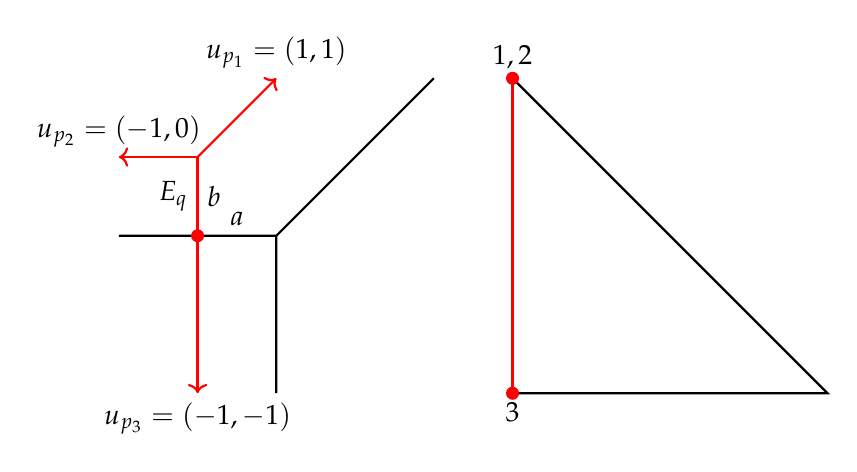
\begin{tikzpicture}[scale=1,transform shape]
      \draw[thick] (-2,0) -- (0,0) -- (0,-2) -- (0,0) -- (2,2);
      \draw[thick,red,->] (-1,1) -- (-2,1);
      \draw[thick,red,->] (-1,1) -- (-1,-2);
      \draw[thick,red,->] (-1,1) -- (0,2);
      \node[anchor=south] (a) at (-0.5,0) {$a$};
      \node[anchor=west] (b) at (-1,0.5) {$b$};
      \node[anchor=east] (eq) at (-1,0.5) {$E_q$};
      \node[anchor=south] (up2) at (-2,1) {$u_{p_2} = (-1,0)$};
      \node[anchor=south] (up1) at (0,2) {$u_{p_1} = (1,1)$};
      \node[anchor=north] (up3) at (-1,-2) {$u_{p_3} = (-1,-1)$};
      \node[circle,fill=red,scale=0.5] (n) at (-1,0) {};
      \draw[thick] (3,-2) -- (7,-2) -- (3,2) -- cycle;
      \draw[red,thick] (3,2) -- (3,-2);
      \node[circle,fill=red,scale=0.5] (n) at (3,-2) {};
      \node[circle,fill=red,scale=0.5] (n) at (3,2) {};
      \node[anchor=south] (p12) at (3,2) {$1,2$};
      \node[anchor=north] (p3) at (3,-2) {$3$};
    \end{tikzpicture}
    \caption{Most generic (tropically) case}
    \label{fig:generic}
  \end{figure}

  Taking the $a \to 0$ limit as in~\Cref{fig:limit1}, then $\tau = \R_{\geq 0}$ and the image of $p_3$ moves along the bottom divisor. In the $b \to 0$ limit, shown in~\Cref{fig:limit2}, we unbreak the curve, and taking the total limit as $(a,b) \to (0,0)$ (see~\Cref{fig:limit3}), we obtain the most general (in the geometric sense) situation.
  \begin{figure}[htpb]
    \centering
    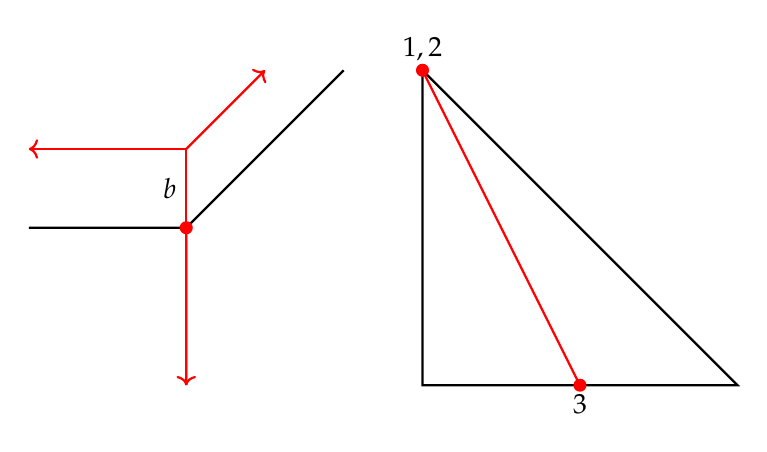
\begin{tikzpicture}[scale=1,transform shape]
      \draw[thick] (-2,0) -- (0,0) -- (0,-2) -- (0,0) -- (2,2);
      \draw[thick,red,->] (0,1) -- (-2,1);
      \draw[thick,red,->] (0,1) -- (0,-2);
      \draw[thick,red,->] (0,1) -- (1,2);
      \node[anchor=east] (b) at (0,0.5) {$b$};
      \node[circle,fill=red,scale=0.5] (n) at (0,0) {};
      \draw[thick] (3,-2) -- (7,-2) -- (3,2) -- cycle;
      \draw[red,thick] (3,2) -- (5,-2);
      \node[circle,fill=red,scale=0.5] (n) at (5,-2) {};
      \node[circle,fill=red,scale=0.5] (n) at (3,2) {};
      \node[anchor=south] (p12) at (3,2) {$1,2$};
      \node[anchor=north] (p3) at (5,-2) {$3$};
    \end{tikzpicture}
    \caption{$a\to 0$ limit of the previous example}
    \label{fig:limit1}
  \end{figure}

  \begin{figure}[htpb]
    \centering
    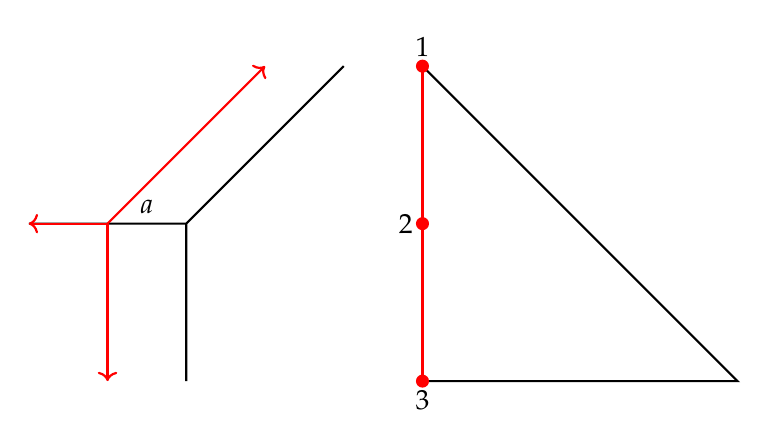
\begin{tikzpicture}[scale=1,transform shape]
      \draw[thick] (-2,0) -- (0,0) -- (0,-2) -- (0,0) -- (2,2);
      \draw[thick,red,->] (-1,0) -- (-2,0);
      \draw[thick,red,->] (-1,0) -- (-1,-2);
      \draw[thick,red,->] (-1,0) -- (1,2);
      \node[anchor=south] (a) at (-0.5,0) {$a$};
      \draw[thick] (3,-2) -- (7,-2) -- (3,2) -- cycle;
      \draw[red,thick] (3,2) -- (3,-2);
      \node[circle,fill=red,scale=0.5] (n) at (3,-2) {};
      \node[circle,fill=red,scale=0.5] (n) at (3,0) {};
      \node[circle,fill=red,scale=0.5] (n) at (3,2) {};
      \node[anchor=south] (p1) at (3,2) {$1$};
      \node[anchor=east] (p2) at (3,0) {$2$};
      \node[anchor=north] (p3) at (3,-2) {$3$};
    \end{tikzpicture}
    \caption{$b\to 0$ limit of the previous example}
    \label{fig:limit2}
  \end{figure}

  \begin{figure}[htpb]
    \centering
    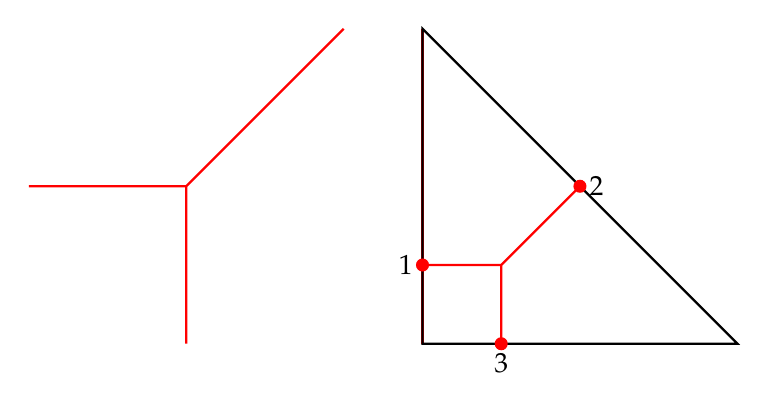
\begin{tikzpicture}[scale=1,transform shape]
      \draw[thick,red] (-2,0) -- (0,0) -- (0,-2) -- (0,0) -- (2,2);
      \draw[red,thick] (3,2) -- (3,-2);
      \draw[thick] (3,-2) -- (7,-2) -- (3,2) -- cycle;
      \node[circle,fill=red,scale=0.5] (n) at (3,-1) {};
      \node[circle,fill=red,scale=0.5] (n) at (5,0) {};
      \node[circle,fill=red,scale=0.5] (n) at (4,-2) {};
      \node[anchor=east] (p1) at (3,-1) {$1$};
      \node[anchor=west] (p2) at (5,0) {$2$};
      \node[anchor=north] (p3) at (4,-2) {$3$};
      \draw[thick,red] (3,-1) -- (4,-1) -- (4,-2) -- (4,-1) -- (5,0);
    \end{tikzpicture}
    \caption{$(a,b)\to (0,0)$ limit of the previous example}
    \label{fig:limit3}
  \end{figure}
  This appears from a degenerating family of general lines. If we consider a family $C \to \A^1_t$ with maps $C \to \P^2$, then $\Sigma_{C_0}$ can be any of the possibilities we discussed before.


Recall that the expanded degneration is point of view was done originally by Jun Li in the case of a smooth divisor and by Ranganathan for a general divisor. In our world, $\ms{Trop}(C)$ defines a cone subdivision $\Sigma$ of $\Sigma_X \times \R_{\geq 0}$ (if $\dim X > 2$, choose a subdivision such that $\Gamma \subset \Sigma(1)$).

In the previous example, let $X = X_{\Sigma}$, which is a blowup of $\P^2 \times \A^1$. Then over $\A^1 \setminus \qty{0}$, we simply obtain $\P^2 \times \A^1 \setminus \qty{0}$, but
\[ X_0 = \bigcup_{\rho \in \Sigma(1)} X_{\Sigma_{\rho}}, \]
where $\Sigma_{\rho}$ is some fan. In the dual picture, we obtain a polyhedral decomposition. Therefore, we obtain a morphism from the expanded degeneration moduli space to our moduli space. An example expanded degeneration is shown in~\Cref{fig:expanded}.
\begin{figure}[htpb]
  \centering
  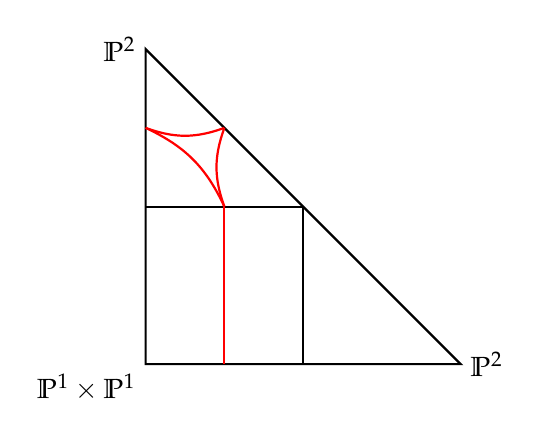
\begin{tikzpicture}[scale=1,transform shape]
    \draw[thick] (0,2) -- (0,-2) -- (4,-2) -- cycle;
    \draw[thick] (0,0) -- (2,0) -- (2,-2);
    \draw[red,thick] (1,-2) -- (1,0);
    \draw[red,thick] (1,0) to [bend left=20] (1,1);
    \draw[red,thick] (1,1) to [bend left=20] (0,1);
    \draw[red,thick] (0,1) to [bend left=20] (1,0);
    \node[anchor=north east] at (0,-2) {$\P^1 \times \P^1$};
    \node[anchor=east] at (0,2) {$\P^2$};
    \node[anchor=west] at (4,-2) {$\P^2$};
  \end{tikzpicture}
  \caption{Example of an expanded degeneration}
  \label{fig:expanded}
\end{figure}

\item This example will have $\tau \neq \R_{\geq 0}^k$. We will choose $X = (\P^1, 0)$ and suppose $C$ has five components in a chain with $C_2, C_3, C_4$ each containing one marked point. Then the contact orders $L_{p_1}, L_{p_2}$ are vertical while $L_{p_3}$ is finite. In the end, we obtain
\[ \tau = \qty{(a,b,c,d) \mid a+b=c+d}. \]
\end{enumerate}
\end{exms}


\begin{defn}
  A stable log map
  \begin{equation*}
    \begin{tikzcd}
      C \ar{d} \ar{r} & X \\
      \Spec (Q \to \C)
    \end{tikzcd}
  \end{equation*}
  is \textit{basic} if and only if $\Sigma_C \to \Sigma_X$ is the universal tropical stable map of some type.
\end{defn}

\subsection{Moduli spaces}
\label{subsec:moduli}

\begin{thm}[Abramovich-Chen, Gross-Siebert]
  There exists a good moduli space of \textbf{basic} stable log maps which is a Deligne-Mumford stack (with log structure) locally of finite type over $\C$ that fulfills the valuative criterion of properness and has a perfect obstruction theory to the stack $\mf{M}$ of log curves with any fine separated log structure on the base. Fixing the topological data
  \[ \beta = (g, \ul{n}, A \in H_2(X)), \]
  the stack is proper and we obtain a virtual fundamental class $[\mc{M}(X, \beta)]^{\mr{vir}}$.
\end{thm}

\section{Artin fans}
\label{sec:artin_fans}

Consider $P = \sigma^{\vee} \cap M$. Suppose that $X_{\sigma}$ has dimension $n$, and then we will define the \textit{toric stack}
\[ \mc{A}_{\sigma} = [X_{\sigma} / \G_m^n]. \]
For any scheme $W$, any map $W \to \mc{A}_{\sigma}$ is a diagram
\begin{equation*}
  \begin{tikzcd}
    Y \ar{r} \ar{d} & X_{\sigma} \ar{d} \\
    W \ar{r} & \mc{A}_{\sigma}
  \end{tikzcd}
\end{equation*}
of a $\G_m^n$-bundle $Y \to W$ and an equivariant map $Y \to X_{\sigma}$.

This has the property that if $\tau \subseteq \sigma$ is a face, then $\mc{A}_{\tau} \subseteq \mc{A}_{\sigma}$ is an open substack. Recall that
\[ \tau^{\vee} \cap M_{\tau} = ((\sigma^{\vee} \cap M) + \tau^{\perp}) / \tau^{\perp}, \]
and therefore $X_{\tau} \times (\C^{\times})^{\codim} \subseteq X_{\sigma}$ is open. For example, we can consider
\[ [\A^1/\G_m] = [\A^1 \times \G_m / \G_m^2] \subseteq [\A^2 / \G_m^2]. \]
Now for any $X = (\ul{X}, \mc{M}_X)$, we obtain a diagram of cones $\Sigma_X$.

\begin{defn}
  The \textit{Artin fan} of $X$ is the algebraic stack
  \[ \mc{X} \coloneqq \varinjlim_{\sigma \in \Sigma_X} \mc{A}_{\sigma}. \]
\end{defn}

The Artin fan algebraizes tropical geometry in the following precise sense.

\begin{prop}
  Assume that $\mc{X}$ has a Zariski covering by various $\mc{A}_{\sigma}$ (for example if $X$ is a Zariski fine separated log scheme which is log-smooth over $\C$). Then for all finite separated log-schemes $T$, there is a canonical bijection
  \[ \Hom_{\ms{log}}(T, \mc{X}) = \Hom_{\ms{cone\ complexes}}(\Sigma_T, \Sigma_X). \]
\end{prop}

As an application, we may define the algebraic stack $\mc{M}(\mc{X})$ of log maps into $\mc{X}$, whose data consists of a domain $C \to \Spec(Q \to \C)$ and a tropical stable map
\begin{equation*}
  \begin{tikzcd}
    \Sigma_C \ar{r} \ar{d} & \Sigma_X \\
    \Hom(Q, \R_{\geq 0}).
  \end{tikzcd}
\end{equation*}

\section{Log Gromov-Witten invariants of fixed type}
\label{sec:fixed_type}

Let $\tau$ be the type of tropical stable maps to $\Sigma_{\mc{X}} = \Sigma_X$.

\begin{defn}
  A \textit{marking} of a stable log map
  \begin{equation*}
    \begin{tikzcd}
      C \ar{r} \ar{d} & X \\
      \Spec(Q \to \C)
    \end{tikzcd}
  \end{equation*}
  by $\tau$ is an identification of $\tau$ with a face of
  \begin{equation*}
  \begin{tikzcd}
      \Sigma_C \ar{r} \ar{d} & \Sigma_X \\
      \Hom(Q, \R_{\geq 0}).
  \end{tikzcd}
  \end{equation*}
\end{defn}

These markings define closed substacks $\mc{M}(\mc{X}, \tau) \subseteq \mc{M}(\mc{X})$. Pulling back to $X$, we obtain the Cartesian diagram
\begin{equation*}
  \begin{tikzcd}
    \mc{M}(X, \tau) \ar{r} \ar{d}{\ep} & \mc{M}(X) \ar{d} \\
    \mc{M}(\mc{X}, \tau) \ar[hookrightarrow]{r} & \mc{M}(\mc{X}).
  \end{tikzcd}
\end{equation*}

In order to have Gromov-Witten invariants, we need a virtual fundamental class. We need the following:
\begin{itemize}
\item The stack $\mc{M}(\mc{X}, \tau)$ is pure-dimensional of dimension $3g-3+k+\dim B - \dim \tau$;
\item The morphism $\mc{M}(X) \to \mc{M}(\mc{X})$ is virtually smooth, so $\mc{M}(X, \tau) \to \mc{M}(\mc{X}, \tau)$ is as well.
\end{itemize}

Now we can define
\[ [ \mc{M}(X, \tau) ]^{\mr{vir}} \coloneqq \ep^{!} [\mc{M}(\mc{X}, \tau)]. \]

\section{Punctured Gromov-Witten invariants and the gluing formalism}
\label{sec:punctured}

\subsection{Rigid tropical curves and virtual decomposition}
\label{subsec:rigid_trop}

\begin{exm}
Let $X' = V(tf_3(z_0,z_1,z_2,z_3) + z_0 \cdots z_2) \subseteq \P^3_{z_0,\ldots,z_3} \times \A^1_t$ be a degeneration of cubic surfaces. We resolve $X'$ to obtain $X$, whose central fiber $X_0$ is a union $\bigcup_3 \Bl_3 \P^2$, as displayed in~\Cref{fig:central_fiber}. Then $\Sigma(X) = \Sigma(X_0)$ is the cone over the unit right triangle.
\begin{figure}[htpb]
  \centering
  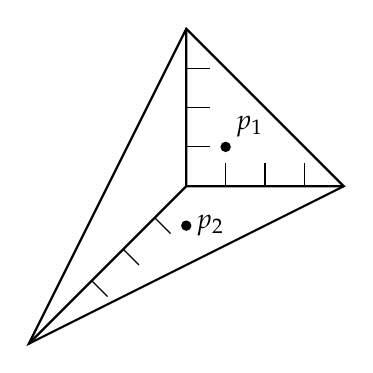
\begin{tikzpicture}[scale=1,transform shape]
    \draw[thick] (0,2) -- (2,0) -- (-2,-2) -- cycle;
    \draw[thick] (0,2) -- (0,0) -- (-2,-2) -- (0,0) -- (2,0);
    \draw (0,0.5) -- (0.3,0.5);
    \draw (0,1) -- (0.3,1);
    \draw (0,1.5) -- (0.3,1.5);
    \draw (0.5,0) -- (0.5,0.3);
    \draw (1,0) -- (1,0.3);
    \draw (1.5,0) -- (1.5,0.3);
    \draw (-0.4,-0.4) -- (-0.2,-0.6);
    \draw (-0.8,-0.8) -- (-0.6,-1);
    \draw (-1.2,-1.2) -- (-1,-1.4);
    \node[fill,circle,scale=0.4] (d1) at (0.5,0.5) {};
    \node[fill,circle,scale=0.4] (d2) at (0,-0.5) {};
    \node[anchor=south west] (p1) at (0.5,0.5) {$p_1$};
    \node[anchor=west] (p2) at (0,-0.5) {$p_2$};
  \end{tikzpicture}
  \caption{Central fiber $X_0$}
  \label{fig:central_fiber}
\end{figure}

Now consider the invariant of $g=0$ curves of degree $d=3$ passing through $p_1, p_2$. There are $12=9+3$ such curves. The two possibilities are shown in~\Cref{fig:posibilities}. The first gives $3 \cdot 3 = 9$ and the second gives $3$ possibilities.
\begin{figure}[htpb]
  \centering
  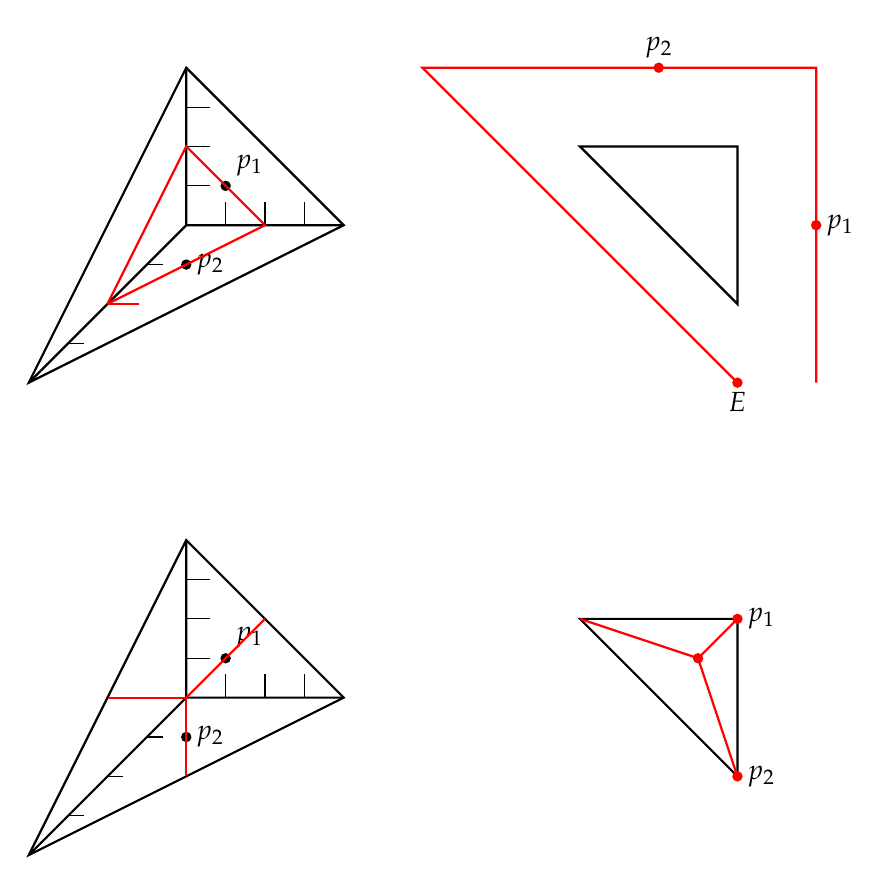
\begin{tikzpicture}[scale=1,transform shape]
    \draw[thick] (0,2) -- (2,0) -- (-2,-2) -- cycle;
    \draw[thick] (0,2) -- (0,0) -- (-2,-2) -- (0,0) -- (2,0);
    \draw (0,0.5) -- (0.3,0.5);
    \draw (0,1) -- (0.3,1);
    \draw (0,1.5) -- (0.3,1.5);
    \draw (0.5,0) -- (0.5,0.3);
    \draw (1,0) -- (1,0.3);
    \draw (1.5,0) -- (1.5,0.3);
    \draw (-0.5,-0.5) -- (-0.3,-0.5);
    \draw[thick,red] (-1,-1) -- (-0.6,-1);
    \draw (-1.5,-1.5) -- (-1.3,-1.5);
    \node[fill,circle,scale=0.4] (d1) at (0.5,0.5) {};
    \node[fill,circle,scale=0.4] (d2) at (0,-0.5) {};
    \node[anchor=south west] (p1) at (0.5,0.5) {$p_1$};
    \node[anchor=west] (p2) at (0,-0.5) {$p_2$};
    \draw[red,thick] (-1,-1) -- (1,0) -- (0,1) -- (-1,-1); 
    \draw[thick] (5,1) -- (7,1) -- (7,-1) -- cycle;
    \draw[red,thick] (7,-2) -- (3,2) -- (8,2) -- (8,-2);
    \node[fill=red,circle,scale=0.4] (e) at (7,-2) {};
    \node[anchor=north] (f) at (7,-2) {$E$};
    \node[fill=red,circle,scale=0.4] (q1) at (8,-0) {};
    \node[fill=red,circle,scale=0.4] (q2) at (6,2) {};
    \node[anchor=south] (p22) at (6,2) {$p_2$};
    \node[anchor=west] (p12) at (8,0) {$p_1$};
    \draw[thick] (0,-4) -- (2,-6) -- (-2,-8) -- cycle;
    \draw[thick] (0,-4) -- (0,-6) -- (-2,-8) -- (0,-6) -- (2,-6);
    \draw (0,-5.5) -- (0.3,-5.5);
    \draw (0,-5) -- (0.3,-5);
    \draw (0,-4.5) -- (0.3,-4.5);
    \draw (0.5,-6) -- (0.5,-5.7);
    \draw (1,-6) -- (1,-5.7);
    \draw (1.5,-6) -- (1.5,-5.7);
    \draw (-0.5,-6.5) -- (-0.3,-6.5);
    \draw (-1,-7) -- (-0.8,-7);
    \draw (-1.5,-7.5) -- (-1.3,-7.5);
    \node[fill,circle,scale=0.4] (d13) at (0.5,-5.5) {};
    \node[fill,circle,scale=0.4] (d23) at (0,-6.5) {};
    \node[anchor=south west] (p13) at (0.5,-5.5) {$p_1$};
    \node[anchor=west] (p23) at (0,-6.5) {$p_2$};
    \draw[thick,red] (0,-6) -- (1,-5);
    \draw[thick,red] (0,-6) -- (-1,-6);
    \draw[thick,red] (0,-6) -- (0,-7);
    \draw[thick] (5,-5) -- (7,-5) -- (7,-7) -- cycle;
    \node[fill=red,circle,scale=0.4] (b) at (6.5,-5.5) {};
    \draw[thick,red] (6.5,-5.5) -- (5,-5);
    \draw[thick,red] (6.5,-5.5) -- (7,-5);
    \draw[thick,red] (6.5,-5.5) -- (7,-7);
    \node[fill=red,circle,scale=0.4] (d14) at (7,-5) {};
    \node[fill=red,circle,scale=0.4] (d24) at (7,-7) {};
    \node[anchor=west] (p14) at (7,-5) {$p_1$};
    \node[anchor=west] (p24) at (7,-7) {$p_2$};
  \end{tikzpicture}
  \caption{Two possibilities (above and below)}
  \label{fig:posibilities}
\end{figure}

We have the decomposition result
\[ [\mc{M}(X_0,\beta)]^{\mr{vir}} = \sum_{\tau\ \text{rigid}} \frac{m_{\tau}}{\abs{\Aut(\tau)}} [\mc{M}(X_0, \tau)]^{\mr{vir}}. \]
In this example, we obtain $12 = (3+3+3)+3$.
\end{exm}

\subsection{Splitting}
\label{subsec:splitting}

Now we will consider $X \to B$ where $B$ is a point or a curve over a log point. Our goal is now to compute
\[ [\mc{M}(X, \tau)]^{\mr{vir}} \]
(whether or not $\tau$ is rigid) by splitting $\tau$ along edges.

\begin{exm}
  We will consider the splittings as in~\Cref{fig:splittings}. Split edges give a pair of ``punctured points'' which in turn produce punctured stable maps.
  \begin{figure}[htpb]
    \centering
    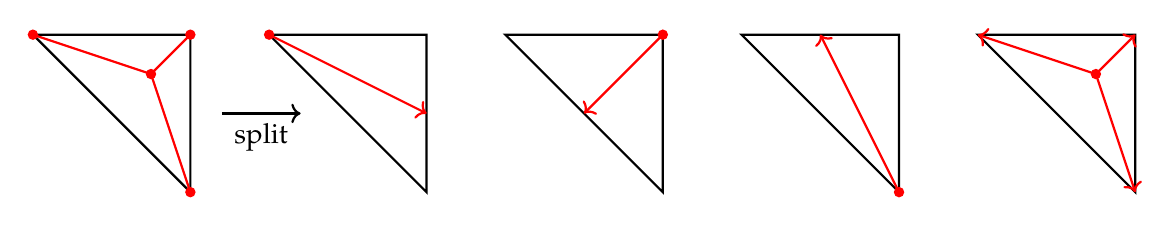
\begin{tikzpicture}[scale=1,transform shape]
      \draw[thick] (0,0) -- (2,0) -- (2,-2) -- cycle;
      \draw[thick,->] (2.4,-1) -- (3.4,-1);
      \node[anchor=north] at (2.9,-1) {split};
      \draw[thick] (3,0) -- (5,0) -- (5,-2) -- cycle;
      \draw[thick] (6,0) -- (8,0) -- (8,-2) -- cycle;
      \draw[thick] (9,0) -- (11,0) -- (11,-2) -- cycle;
      \draw[thick] (12,0) -- (14,0) -- (14,-2) -- cycle;
      \node[fill=red,circle,scale=0.4] at (1.5,-0.5) {};
      \node[fill=red,circle,scale=0.4] at (0,0) {};
      \node[fill=red,circle,scale=0.4] at (2,-2) {};
      \node[fill=red,circle,scale=0.4] at (2,0) {};
      \node[fill=red,circle,scale=0.4] at (3,0) {};
      \node[fill=red,circle,scale=0.4] at (8,0) {};
      \node[fill=red,circle,scale=0.4] at (11,-2) {};
      \node[fill=red,circle,scale=0.4] at (13.5,-0.5) {};
      \draw[thick,red] (1.5,-0.5) -- (0,0);
      \draw[thick,red] (1.5,-0.5) -- (2,0);
      \draw[thick,red] (1.5,-0.5) -- (2,-2);
      \draw[thick,red,->] (3,0) -- (5,-1);
      \draw[thick,red,->] (8,0) -- (7,-1);
      \draw[thick,red,->] (11,-2) -- (10,0);
      \draw[thick,red,->] (13.5,-0.5) -- (12,0);
      \draw[thick,red,->] (13.5,-0.5) -- (14,0);
      \draw[thick,red,->] (13.5,-0.5) -- (14,-2);
    \end{tikzpicture}
    \caption{Splittings $\tau_1, \tau_2, \tau_3, \tau_4$ of $\tau$}
    \label{fig:splittings}
  \end{figure}
\end{exm}

\begin{thm}
  There is a Cartesian diagram
  \begin{equation*}
    \begin{tikzcd}
      \mc{M}(X, \tau) \ar{r} \ar{d} & \prod_i \mc{M}(X, \tau_i) \ar{d} \\
      \mc{M}^{\mr{ev}}(\mc{X}, \tau) \ar{r}{\delta^{\mr{ev}}} & \prod_i \mc{M}^{\mr{ev}}(\mc{X}, \tau_i)
    \end{tikzcd}
  \end{equation*}
  where the vertical arrows are virtually smooth. The ``ev'' makes the bottom arrow representable and finite, and is defined by
  \[ \mc{M}^{\mr{ev}}(\mc{X}, \tau) = \mc{M}(\mc{X}, \tau) \times_{\mc{X}^k} X^k, \]
  where there is one choice for each puncture from splitting or node to split. We should note that the morphism $X \to \mc{X}$ is smooth (in the ordinary sense), so the fiber product is a harmless operation.
\end{thm}

\begin{cor}
If we know $\delta^{\mr{ev}}_* [\mc{M}^{\mr{ev}}(\mc{X}, \tau)]$ on $\prod_i \mc{M}^{\mr{ev}}(\mc{X}, \tau_i)$, we obtain a gluing formula $\on{GW}(\tau) = F(\on{GW}(\tau_i))$.
\end{cor}

\begin{thm}[Gluing theorem]
  There is an fs-Cartesian diagram
  \begin{equation*}
    \begin{tikzcd}
      \wt{\mc{M}'}^{\mr{ev}}(\mc{X}, \tau) \ar{r} \ar{d}{\mr{ev}} & \prod_i \wt{\mc{M}'}^{\mr{ev}}(\mc{X}, \tau_i) \ar{d}{\mr{ev}} \\
      X^k \ar{r}{\Delta} & X^k \times X^k.
    \end{tikzcd}
  \end{equation*}
  Here, the tilde gives a bigger log structure, and the prime changes the non-reduced structure. Finally, fs-Cartesian means that the fiber product is modeled on the fiber product of cones in the following sense for toric varieties:
  \[ X_{\sigma_1} \times^{\mr{fs}}_{X_{\tau}} X_{\sigma_2} = X_{\sigma_1 \times_{\tau} \sigma_2}. \]
  For example, if $X_{\tau} = \A^2$ and $X_{\sigma_1}, X_{\sigma_2}$ are lines with different slopes, then the fs-fiber product is empty.
\end{thm}

By work of Yixian Wu, the gluing stratum of $X$ (contained in type $\tau$) are \textbf{toric}, so we obtain the gluing formula
\[ \delta_*^{\mr{ev}}[\mc{M}^{\mr{ev}}(\mc{X}, \tau)] = \sum_{\omega = (\omega_i) \supseteq \tau_i} (\text{tropical multiplicity}) \cdot \prod_i [\mc{M}^{\mr{ev}}(\mc{X}, \omega_i)]. \]
The $\omega$ are obtained as solutions to perturbation problems for $\tau$ via displacement along edges. There is a similar formula in a different setting due to Venugopalan-Woodward.

\begin{exm}
  Consider a degeneration of $\P^1 \times \P^1$ to $\bigcup_2 \P^2$ via the cone over the skeleton in~\Cref{fig:skeleton}.
  \begin{figure}[htpb]
    \centering
    \begin{tikzpicture}[scale=1,transform shape]
      \draw[thick] (-1,0) -- (0,0) -- (0,-1) -- (0,0) -- (1,1) -- (2,1) -- (1,1) -- (1,2);
    \end{tikzpicture}
    \caption{Skeleton}
    \label{fig:skeleton}
  \end{figure}
  If we consider curves of bidegree $(1,1)$, then $\tau$ is simply the skeleton. We can split along the diagonal edge and then perturb by the tangent vector $\xi = (1,0)$. The possibilities for $\omega_1, \omega_2$ are shown in~\Cref{fig:perturb}.
  \begin{figure}[htpb]
    \centering
    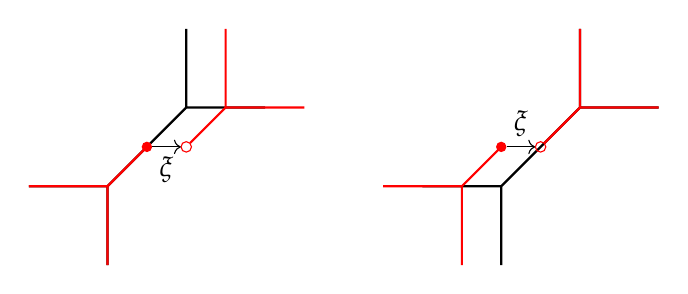
\begin{tikzpicture}[scale=1,transform shape]
      \draw[thick] (-1,0) -- (0,0) -- (0,-1) -- (0,0) -- (1,1) -- (2,1) -- (1,1) -- (1,2);
      \node[circle,fill=red,scale=0.4] (a) at (0.5,0.5) {};
      \node[circle,draw=red,scale=0.4] (b) at (1,0.5) {};
      \draw[thick,red] (-1,0) -- (0,0) -- (0,-1) -- (0,0) -- (0.5,0.5);
      \draw[thick,red] (b) -- (1.5,1) -- (2.5,1) -- (1.5,1) -- (1.5,2);
      \draw[->] (a) -- (b);
      \node[anchor=north] at (0.75,0.5) {$\xi$};
      \draw[thick] (4,0) -- (5,0) -- (5,-1) -- (5,0) -- (6,1) -- (7,1) -- (6,1) -- (6,2);
      \node[circle,fill=red,scale=0.4] (c) at (5,0.5) {};
      \node[circle,draw=red,scale=0.4] (d) at (5.5,0.5) {};
      \draw[thick,red] (3.5,0) -- (4.5,0) -- (4.5,-1) -- (4.5,0) -- (5,0.5);
      \draw[thick,red] (d) -- (6,1) -- (7,1) -- (6,1) -- (6,2);
      \draw[->] (c) -- (d);
      \node[anchor=south] at (5.25,0.5) {$\xi$};
    \end{tikzpicture}
    \caption{Possible perturbations of the skeleton}
    \label{fig:perturb}
  \end{figure}
\end{exm}

\subsection{Punctured curves and punctured GW invariants}
\label{subsec:punctured}

\begin{defn}
A \textit{punctured curve} $C^{\circ} = (\ul{C}, \mc{M}_{C^{\circ}}) \to \Spec(Q \to \C)$ is defined almost as a log curve is before, but instead of $Q \oplus \N$ at marked points, we admit submonoids $Q^{\circ} \subseteq Q \oplus \Z$ such that $Q \oplus \N \subseteq Q^{\circ}$ and for any $(g,k)$ with $k < 0$ implies that $\alpha(q,k) = 0$. This is a fine log structure, but is not separated.
\end{defn}

\begin{exm}
  Let $C = C_1 \cup C_2$ with node $q$. Let $\iota \colon C_1 \hookrightarrow C$ and $q = \iota(p)$. Then
  \[ \mc{M}_{C^{\circ}} = \iota^* \mc{M}_C \]
  is a puncturing at $p$.
\end{exm}

\begin{defn}
A \textit{stable punctured map} is a stable map $C^{\circ} \to X$ such that $\ol{\mc{M}}_{C^{\circ}, p}$ is generated by $Q \oplus \N$ and $\ol{f}^{\flat}(\ol{\mc{M}}_{X,f(p)})$ for all punctures $p$.
\end{defn}

The second condition on generation of $\ol{\mc{M}}_{C^{\circ},p}$ is equivalent tropically to saying that the bounded leg $L_p$ for the punctured point $p$ extends \textbf{as far as} possible. After some work, we may define tropical punctured maps, their types, and moduli spaces of punctured stable maps as before.

\begin{exm}
  Recall the example of $\Bl_1(\P^1 \times \P^1)$, where we blow up on the interior of one of the boundary divisors. Then we consider a line degenerating to the strict transform of the blown up boundary divisor. We will have two marked points and one puncture which moves to the exceptional divisor. The classical and tropical pictures are shown in~\Cref{fig:punctured}.
  \begin{figure}[htpb]
    \centering
    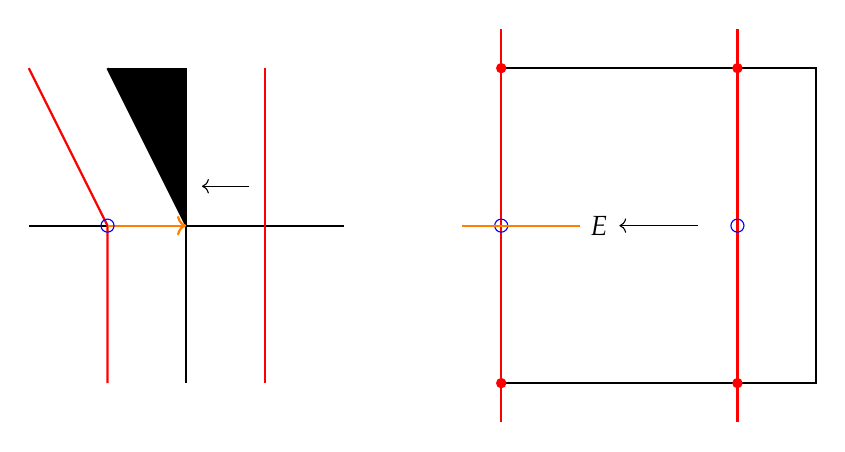
\begin{tikzpicture}[scale=1,transform shape]
      \draw[thick] (0,2) -- (0,-2);
      \draw[thick] (2,0) -- (-2,0);
      \fill[fill=black] (0,0) -- (-1,2) -- (0,2) -- cycle;
      \draw[thick] (0,0) -- (-1,2);
      \draw[red,thick] (1,-2) -- (1,2);
      \draw[->] (0.8,0.5) -- (0.2,0.5);
      \draw[red,thick] (-1,-2) -- (-1,0) -- (-2,2);
      \draw[orange,thick,->] (-1,0) -- (0,0);
      \node[circle,draw=blue,scale=0.5] at (-1,0) {};
      \draw[thick] (4,2) -- (8,2) -- (8,-2) -- (4,-2);
      \draw[thick,red] (7,-2.5) -- (7,2.5);
      \draw[thick,red] (4,-2.5) -- (4,2.5);
      \node[circle,fill=red,scale=0.4] at (7,2) {};
      \node[circle,fill=red,scale=0.4] at (7,-2) {};
      \node[circle,draw=blue,scale=0.5] at (7,0) {};
      \node[circle,draw=blue,scale=0.5] at (4,0) {};
      \node[circle,fill=red,scale=0.4] at (4,2) {};
      \node[circle,fill=red,scale=0.4] at (4,-2) {};
      \draw[->] (6.5,0) -- (5.5,0);
      \draw[thick,orange] (3.5,0) -- (5,0);
      \node[anchor=west] at (5,0) {$E$};
    \end{tikzpicture}
    \caption{A comparison of punctured and unpunctured invariants. Punctures are blue and the exceptional divisor is orange.}
    \label{fig:punctured}
  \end{figure}

  The virtual dimension is $0$, and in fact we have
  \[ \deg [\mc{M}(X, \tau)]^{\mr{vir}} = 1. \]
\end{exm}

As an application, we may consider a degeneration $X \to S$ of a Calabi-Yau or $(X,D)$ a log Calabi-Yau. Let $B \subseteq \Sigma(X)$ be the Kontsevich-Soibelman skeleton, which is an integral affine manifold. From $1$-punctured invariants, we obtain a wall structure on $B$ (for example in the previous example, consider $E$) with walls swept out by images of tropical punctured maps of wall type, which are not defined here. From the wall structure, we produce an intrinsic mirror ring from $1$-punctured invariants with up to $2$ marked points. Then the formula of Yixian Wu tells us that enumerative and algebraic wall crossings are the same. For a reference, see \textit{The canonical wall structure and intrinsic mirror symmetry} by Gross and Siebert.

\chapter{A spin on Hurwitz theory and topological recursion (Danilo Lewanski)}
\label{cha:lewanski}

The impatient reader may skip to~\Cref{fig:summary} for a flowchart which summarizes this chapter.

\section{Hurwitz theory}
\label{sec:hurwitz}

We are interested in studying $d:1$ branched covers $f \colon C \to D$ from a curve $C$ of genus $g$ to a curve $D$ of genus $h$. Then we know that $f$ has $k$ ramification points, above which we see ramification profiles, which are partitions $\mu^i$ of $d$. Therefore, \textit{Hurwitz theory} enumerates branched coverings of Riemann surfaces with specified ramification data. There are several common specializations:
\begin{enumerate}
\item We choose one or two partitions to be special, and their parts are variables. All other ramification profiles are of the same type.
\item We can also set $h=0$, so we are looking for coverings of $\P^1$.
\end{enumerate}

\begin{defn}
  Let $B$ be a connected and compact Riemann surface and fix $x_1, \ldots, x_k \in B$ and partitions $\mu^1, \ldots, \mu^k$. Then the \textit{Hurwitz number} is defined to be
  \[ H_d(B; \mu^1, \ldots, \mu^k) \coloneqq \sum_{[f]} \frac{1}{\abs{\Aut(f)}}, \]
  where the sum is over equivalence classes $[f]$ of branched covers $f$. We will write $H_d^{\circ}$ to enforce connected domains and $H_d^{\bullet}$ to have possibly disconnected domains.
\end{defn}

\begin{exms}\leavevmode
  \begin{enumerate}
  \item Consider the map
  \[ f \colon \P^1 \to \P^1 \qquad z \mapsto z^d. \]
  Then we know that $\Aut(f) = \mu_d$ is the $d$-th roots of unity, and therefore
  \[ H_d^{\circ} (\P^1, (d), (d)) = \frac{1}{d}. \]
  \item Let $E$ be given by the equation $y^2 = x^3 + ax+b$. There is a unique map $f \colon E \to \P^1$ of degree $2$. This map has a unique involution given by $y \mapsto -y$, and therefore
  \[ H^{\circ}(\P^1, (2), (2), (2), (2)) = \frac{1}{2}. \]
  \end{enumerate}
\end{exms}

\begin{exer}
  We list a few more invariants:
  \begin{enumerate}
  \item $H^{\circ}(S^1 \times S^1; (2,1)^4) = 9$;
    \item Compute $H^{\circ}(\Sigma_2; (3), (2,1)^6)$ and $H^{\circ}(\Sigma_5, (3)^4, (2,1)^6)$.
  \end{enumerate}
\end{exer}

It is unclear from the specification of the problem that a single cover even exists for a given $g, h, \mu^i$. We of course do have a classically known linear condition.

\begin{thm}[Riemann-Hurwitz]
  For any $f$, we have
  \[ 2g-2 = d(2h-2) + \sum_{i=1}^k (d-\ell(\mu^i)). \]
\end{thm}

This theorem is proved by lifting a triangulation of $B$ passing through the $x_i$. Any cover satisfies this formula, but not all data which satisfy the formula admit a connected covering.

\subsection{Spin Hurwitz numbers}
\label{subsec:spin}

\begin{defn}
A \textit{spin structure} on $B$ is a holomorphic line bundle $\theta$ on $B$ such that $\theta^{\otimes 2} \cong \omega_B$.
\end{defn}

\begin{exms}\leavevmode
\begin{enumerate}
\item Let $B = \P^1$. Then there is a unique spin structure given by $\mc{O}(-1)$.
\item If $\theta$ is a spin structure on $B$ and all $\mu_j^i$ are odd, then
  \[ \theta_f \colon f^* \theta \otimes \mc{O}\qty(\sum_{i,j} \frac{(\mu_j^i-1)}{2} x_i^{(j)}) \]
  is a spin structure on the domain of $f$. Here, $x_i^{(j)}$ is the $j$-th preimage of $x_i$. This follows from the formula
  \[ \omega_C \cong f^* \omega_B \otimes \mc{O}\qty(\sum_{i,j} (\mu_j^i-1) x_i^{(j)}). \]
  Note that if we compute the degree of both sides, we obtain the Riemann-Hurwitz formula.
\end{enumerate}
\end{exms}

\begin{defn}
  The \textit{spin Hurwitz number} is defined by
  \[ H_d(B, \theta; \mu^1, \ldots, \mu^k) \coloneqq \sum_{[f]} \frac{(-1)^{\mr{Arf}(f)}}{\abs{\Aut(f)}}, \]
  where $\mr{Arf}(f \colon C \to B) = h^0(C, \theta_f)$.
\end{defn}

It turns out that all spin Hurwitz numbers are positive, but this is somewhat unexpected. However, we can enumerate spin structures on curves.
\begin{thm}
On any curve of genus $g$, there are $2^{g-1}(2^g+1)$ even spin structures and $2^{g-1} (2^g-1)$ odd spin structures.
\end{thm}
In~\Cref{tab:even_odd}, we can see these numbers for low genus.
\begin{table}[htpb]
  \centering
  \caption{Enumeration of even and odd spin structures}
  \label{tab:even_odd}
  \begin{tabular}{ccc}
    \toprule
    $g$ & even spin structures & odd spin structures \\
    \midrule
    $0$ & $1$ & $0$ \\
    $1$ & $3$ & $1$ \\
    $2$ & $10$ & $6$ \\
    $3$ & $36$ & $28$ \\
    \bottomrule
  \end{tabular}
\end{table}

\subsection{Burnside formula}
\label{subsec:burnside}

\begin{prob}
Computing Hurwitz or spin Hurwitz numbers directly from the geometry is extremely hard.
\end{prob}

The solution to this is that there exists an automorphism-preserving bijection
\[ \qty{\Centerstack{{isomorphism classes $f \colon C \to B$} {$C$ possibly disconnected} {ramified at $x_i$} {ramification data $\mu^i$} {$\theta_f$ even/odd}}} \xleftrightarrow{\varphi} \qty{\Centerstack{{Monodromy representations} {$\rho \colon \pi_1(B \setminus \qty{x_i}, y) \to \mf{S}_d$} {of type $(\mu^1, \ldots, \mu^k)$} {with/without lift to $\wt{\mf{S}}_d$}}}, \]
where
\[ \wt{\mf{S}}_d = \ev{t_1, \ldots, t_{d-1}, \ep \mid \ep^2=1, t_j^2 = \ep, (t_jt_{j+1})^3 = \ep, t_jt_k^2=\ep \text{ for } \abs{j-k} > 1} \]
is an extension
\[ 0 \to \Z/2\Z \to \wt{\mf{S}}_d \to \mf{S}_d \to 0 \]
defined by Giachetto-Kramer-Lewanski.

For example, we can now compute
\[ H_d^{\bullet}(\P^1; \mu^1, \ldots, \mu^k) = \frac{1}{d!} [\mr{id}] C_{\mu^1} \cdots C_{\mu^k} \mf{k}^h, \]
where
\[ C_{\mu} \coloneqq \sum_{\substack{\sigma \in \mf{S}_d \\ \text{cycle type} = \mu}} \sigma. \]
Also, this $\mf{k}^h$ is defined in Cavalieri-Miks and is a correction factor.
For example, $C_{(2,1,\ldots,1)}$ is the sum of all transpositions and $C_{(d)}$ is the sum of all cycles of length $d$. This formula is can be generalized to the spin setting, but we will instead give a different formula. We will now restate the formula using characters.

\begin{defn}
  For a partition $\lambda$, define
  \[ F_{\lambda} \coloneqq \frac{\dim(\lambda)}{d!} \sum_{\mu \colon \abs{\mu} = \abs{\lambda}} \chi_{\lambda}(\mu) C_{\mu}. \]
\end{defn}
By orthogonality of characters, we obtain $F_{\lambda} F_{\varphi} = F_{\lambda} \delta_{\lambda \varphi}$, so the $F_{\lambda}$ form an idempotent basis. Inverting this formula, we obtain
\[ C_{\mu} = \sum_{\lambda} \abs{C_{\mu}} \frac{\chi_{\lambda}(\mu)}{\dim(\lambda)} F_{\lambda}, \]
and inserting us into the previous formula, we obtain

\begin{thm}[Burnside formula]
  \[ H^{\bullet}(B;\mu^1, \ldots, \mu^k) = \sum_{\lambda} \qty(\frac{\prod^k \abs{C_{\mu^i}} \chi_{\lambda \vdash d}(\mu^i)}{\dim(\lambda)}) \qty(\frac{\dim(\lambda)}{d!})^{2-2h}. \]
\end{thm}

In the spin setting, there is the following theorem:

\begin{thm}
  \[ H_d^{\bullet}(B, \theta; \mu^1, \ldots,\mu^k) = 2^A \sum_{\substack{\lambda \vdash d \\ \text{strict}}} (-1)^{\ell(\lambda) \cdot h_0(B, \theta)} \prod_{i=1^k} \abs{\wt{C}_{\mu^i}} \frac{\wt{\chi}_{\lambda}(\mu^i)}{\dim(\lambda)} \qty(\frac{\dim(\lambda)}{2^{p(\lambda)/2}})^{2-2h}, \]
  where $\wt{\chi}, \wt{C}$ are the same as the ones without tildes but for $\wt{\mf{S}}_d$ and
  \[ p(\lambda) = \begin{cases}
                    1 & \ell(\lambda) \text{ odd} \\
                    0 & \ell(\lambda) \text{ even}.
                  \end{cases} \]
                Finally, here
                \[ A= \sum_{i=1}^k \frac{\ell(\mu^i) - d}{2} - (2-2h). \]
                It should also be noted that strict partitions must be strictly decreasing.
\end{thm}

We will now fix a positive integer $r$. Classically, we consider $(r+1)$-completed cycles and Hurwitz numbers with $B = \P^1$. We will write
\[ \mu^1 \coloneqq (\mu_1, \ldots, \mu_n), \]
and all other $\mu^i$ will be
\[ \mu^i = (r+1, 1, \ldots, 1) + \text{correction terms}, \]
where the correction terms generate $\frac{1}{2\sinh(z/2)}$. In the spin setting, we will consider $B = (\P^1, \mc{O}(-1))$, force the $\mu_i$ to be odd, and have the correction terms generate $\frac{1}{2} \coth(z/2)$.

\begin{rmk}
We should note that we would like to generalize the Gromov-Witten/Hurwitz correspondence of Okounkov-Pandharipande to the spin case, where we consider spin $(r+1)$-completed cycles. The other motivation is the Zvonkine conjecture/theorem relating to the ELSV formula.
\end{rmk}

\begin{defn}
  Define the function
  \[ \phi \colon Z \Q[\mf{S}_d] \to \Q^{\mc{P}_d} \qquad C_{\mu} \mapsto \mathbf{f}_{\mu}, \]
  where
  \[ \mathbf{f}_{\mu} \coloneqq \abs{C_{\mu}} \frac{\chi_{\bullet}(\mu)}{\dim(\bullet)} = \frac{\prod \mathbf{p}_{\mu_i}}{\prod \mu_i} + \text{lower order terms}. \]
  Adding a tilde to everything, we get the spin version. Here, we have
  \[ \mathbf{p}_{\mu} = \prod_{i=1}^n p_{\mu_i} \qquad p_S(\lambda) \coloneqq \sum_{k>0} \qty[\qty(\lambda_k-k+\frac{1}{2})^s - \qty(-k+\frac{1}{2})^s]. \]
  In the spin case, we define
  \[ \wt{p}_S(\lambda) = \sum_{k>0} \lambda_k^s. \]
  Then the \textit{completed cycles} are defined to be
  \[ \ol{C}_{r+1} \coloneqq \phi^{-1} \qty(\frac{\mathbf{p}_{(r+1,1,\ldots,1)}}{r+1}). \]
  In the spin case, the definition is the same.
\end{defn}

\begin{defn}
  We will define the \textit{$(r+1)$-completed cycles Hurwitz numbers} by
  \[ h_{g;\mu}^{\bullet, r} \coloneqq \frac{\Aut(\mu)}{b!} H_d^{\bullet}(\P^1, \mu, (\ol{C}_{r+1})^b), \]
  where
  \[ b_{\mr{RH}} = \frac{2g-2+\ell(\mu)+d}{r}. \]
  In the spin case, simply consider $(\P^1, \mc{O}(-1))$ and add a tilde to everything,
\end{defn}

These are very hard to compute, and closed formulae are very hard, so we instead develop recursions, such as cut and join, topological recursion, and the Toda equations. The following result was conjectured by Pandharipande.

\begin{thm}[Okounkov]
  The series
  \[ \mc{H}(x,y) \coloneqq \sum_{g=0,d=1} h_{g;(1)^d}^{\circ,r=1} x^{2g+2d-2}y^d \]
  satisfies the equation
  \[ \qty(y \dv{y})^2 \mc{H}(x,y) = ye^{\mc{H}(x,ye^x)-2\mc{H}(x,y) + \mc{H}(x,ye^{-x})}, \]
  which is the first equation of the Toda lattice.
\end{thm}

\subsection{Operator interpretation of Hurwitz numbers}
\label{subsec:fockspace}

One of the main ingredients in this is a Fock space interpretation of Hurwitz numbers $h_{g;\mu,\nu}^{\bullet,r}$ as a vacuum expectation value of the operator
\[ \ev{\alpha_{\mu_1} \circ \cdots \circ \alpha_{\mu_n} \frac{(\mc{F}_{r+1})^b}{b!} \alpha_{-\nu_1} \circ \cdots \circ \alpha_{-\nu_m}}, \]
where
\[ b = \frac{2g-2+\ell(\mu) + \ell(\nu)}{r} \]
is determined by the Riemann-Hurwitz formula.

\begin{defn}
  The \textit{vacuum} $v_{\emptyset}$ is defined to be the Maya diagram in~\Cref{fig:vacuum}.
  \begin{figure}[htpb]
    \centering
    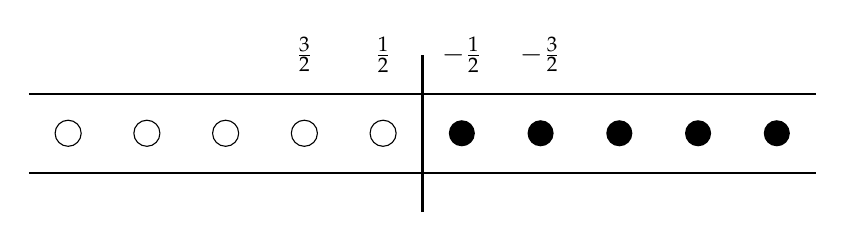
\begin{tikzpicture}[scale=1,transform shape]
      \draw[thick] (-5,1) -- (5,1);
      \draw[thick] (-5,0) -- (5,0);
      \draw[thick] (0,-0.5) -- (0,1.5);
      \node[fill,circle] at (0.5,0.5) {};
      \node[fill,circle] at (1.5,0.5) {};
      \node[fill,circle] at (2.5,0.5) {};
      \node[fill,circle] at (3.5,0.5) {};
      \node[fill,circle] at (4.5,0.5) {};
      \node[circle,draw] at (-0.5,0.5) {};
      \node[circle,draw] at (-1.5,0.5) {};
      \node[circle,draw] at (-2.5,0.5) {};
      \node[circle,draw] at (-3.5,0.5) {};
      \node[circle,draw] at (-4.5,0.5) {};
      \node at (0.5,1.5) {$-\frac{1}{2}$};
      \node at (1.5,1.5) {$-\frac{3}{2}$};
      \node at (-0.5,1.5) {$\frac{1}{2}$};
      \node at (-1.5,1.5) {$\frac{3}{2}$};
    \end{tikzpicture}
    \caption{Vacuum vector}
    \label{fig:vacuum}
  \end{figure}
\end{defn}

Note that there exists a bijection between partitions and the charge zero sector of Maya diagrams (where the are the same number of black stones on the left and white stones on the right). For example, the partition $(3,2,2)$ corresponds to the Maya diagram in~\Cref{fig:maya322};
\begin{figure}[htpb]
  \centering
  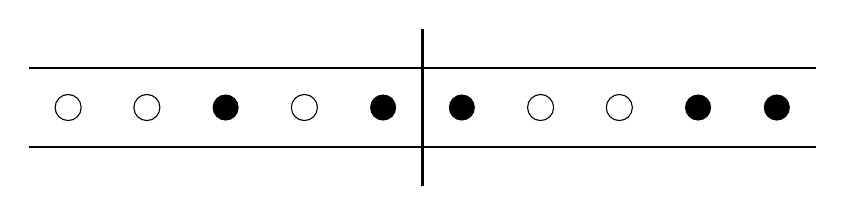
\begin{tikzpicture}[scale=1,transform shape]
    \draw[thick] (-5,1) -- (5,1);
    \draw[thick] (-5,0) -- (5,0);
    \draw[thick] (0,-0.5) -- (0,1.5);
    \node[fill,circle] at (0.5,0.5) {};
    \node[draw,circle] at (1.5,0.5) {};
    \node[draw,circle] at (2.5,0.5) {};
    \node[fill,circle] at (3.5,0.5) {};
    \node[fill,circle] at (4.5,0.5) {};
    \node[circle,fill] at (-0.5,0.5) {};
    \node[circle,draw] at (-1.5,0.5) {};
    \node[circle,fill] at (-2.5,0.5) {};
    \node[circle,draw] at (-3.5,0.5) {};
    \node[circle,draw] at (-4.5,0.5) {};
  \end{tikzpicture}
  \caption{Vector corresponding to $\lambda = (3,2,2)$}
  \label{fig:maya322}
\end{figure}

Now we will define the operator
\[ \alpha_m \coloneqq \sum_{k \in \Z+\frac{1}{2}} :\psi_{k-m} \psi_k^{\dag}: \in \wh{\mf{gl}(\infty)}, \]
where $\psi_k^{\dag}$ attempts to remove a black stone from position $k$, $\psi_{k-m}$ attempts to drop a black stone in position $k-m$, and
\[ \wh{\mf{gl}(\infty)} \coloneqq \qty{c + \sum_{r,s} a_{r,s} :\psi_{-r} \psi_s^{\dag}: \mid a_{r,s} = 0 \text{ if } \abs{r-s} \gg 0}. \]
Note that even though $\alpha_m$ is an infinite sum, when applied to any charge zero Maya diagram, it only has finitely many nonzero elements. Also, recall that the normal ordering is defined by
\[ :\psi_i \psi_j^{\dag}: = \begin{cases}
                              \psi_i \psi_j^{\dag} & j > 0 \\
                              -\psi_j^{\dag} \psi_i & j < 0.
                            \end{cases} \]
We can also build Maya diagrams from partitions by using the Russian notation for partitions as seen in~\Cref{fig:russianmaya}.
\begin{figure}[htpb]
  \centering
  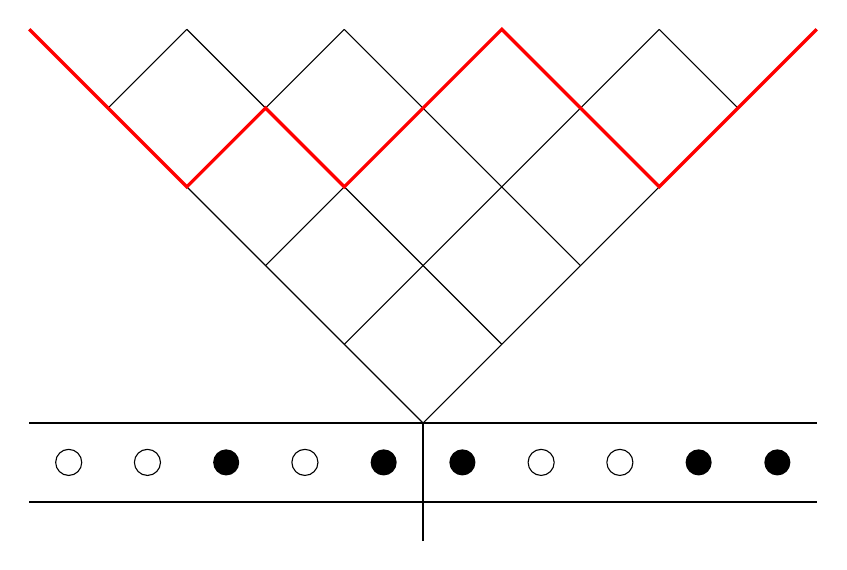
\begin{tikzpicture}[scale=1,transform shape]
    \draw[thick] (-5,1) -- (5,1);
    \draw[thick] (-5,0) -- (5,0);
    \draw[thick] (0,-0.5) -- (0,1);
    \node[fill,circle] at (0.5,0.5) {};
    \node[draw,circle] at (1.5,0.5) {};
    \node[draw,circle] at (2.5,0.5) {};
    \node[fill,circle] at (3.5,0.5) {};
    \node[fill,circle] at (4.5,0.5) {};
    \node[circle,fill] at (-0.5,0.5) {};
    \node[circle,draw] at (-1.5,0.5) {};
    \node[circle,fill] at (-2.5,0.5) {};
    \node[circle,draw] at (-3.5,0.5) {};
    \node[circle,draw] at (-4.5,0.5) {};
    \draw[thin] (-5,6) -- (0,1) -- (5,6);
    \draw[thin] (-3,6) -- (1,2);
    \draw[thin] (-1,6) -- (2,3);
    \draw[thin] (1,6) -- (3,4);
    \draw[thin] (3,6) -- (4,5);
    \draw[thin] (3,6) -- (-1,2);
    \draw[thin] (1,6) -- (-2,3);
    \draw[thin] (-1,6) -- (-3,4);
    \draw[thin] (-3,6) -- (-4,5);
    \draw[red,very thick] (-5,6) -- (-3,4) -- (-2,5) -- (-1,4) -- (0,5) -- (1,6) -- (2,5) -- (3,4) -- (5,6);
  \end{tikzpicture}
  \caption{Maya diagram and Russian partition notation corresponding to $\lambda = (3,2,2)$}
  \label{fig:russianmaya}
\end{figure}
If we apply $\alpha_2$, we obtain
\[ \alpha_2 v_{\lambda} = - v_{(3,1,1)} + v_{(3,2)}. \]
This is exactly the same as the Murnaghan-Nakayama rule, which implies that
\[ \alpha_{-\mu_1} \circ \cdots \circ \alpha_{-\mu_n} = \sum_{\abs{\lambda} = \abs{\mu}} \chi_{\mu}(\lambda) v_{\lambda}. \]
The $\alpha_n$ also satisfy the relations
\[ [\alpha_n, \alpha_m] = n \delta_{n+m}. \]

It now remains to define $\mc{F}_{r+1}$ such that its eigenvalue is the completed cycle. We want
\[ \mc{F}_{r+1} v_{\lambda} = \mathbf{p}_{r+1}(\lambda) v_{\lambda}, \]
and the correct definition is
\[ \mc{F}_{r+1} \coloneqq \sum_{k \in \Z+\frac{1}{2}} k^{r+1} :\psi_k \psi_k^{\dag}: \in \wh{\mf{gl}(\infty)}. \]

We will also define other operators
\[ \mc{E}_m(z) = \sum_{k \in \Z + \frac{1}{2}} e^{z \qty(k-\frac{m}{2})} :\psi_{k-m} \psi_k^{\dag}: + \frac{\delta_m}{\zeta(z)}, \]
where $\zeta(z) = 2 \sinh\qty(\frac{z}{2})$. As studied by Okounkov-Pandharipande, these satisfy the relation
\[ [\mc{E}_a(z), \mc{E}_b(w)] = \zeta \qty(\begin{vsmallmatrix} a & b \\ z & w \end{vsmallmatrix}) \mc{E}_{a+b}(z+w). \]
Note that if we set $z = 0$, $\mc{E}_m(0) = \alpha_m$ and if we set $m=0$, then
\[ (r+1)! [z^{r+1}] \mc{E}_m(z) = \mc{F}_{r+1}. \]

In the spin setting, we may define
\[ \mc{E}_m^{\mr{spin}}(z) = \frac{1}{2} \sum_{k \in \Z} e^{\qty(k+\frac{m}{2})z} (-1)^k \varphi_k \varphi_{-k-m} + \frac{\delta_m}{4} \coth\qty(\frac{z}{2}), \]
where we define
\[ \varphi_m \coloneqq \frac{1}{\sqrt{2}} \qty[\psi_{m-\frac{1}{2}} + (-1)^m \psi_{-m-\frac{1}{2}}^{\dag}] \]
to be the \textit{uncharged fermion}. The commutation relations become
\[ [\mc{E}_a^{\mr{spin}}(z), \mc{E}_b^{\mr{spin}}(w)] = \frac{1}{2} \zeta \qty(\begin{vsmallmatrix} a & b \\ z & w \end{vsmallmatrix}) \mc{E}_{a+b}^{\mr{spin}}(z+w) + \frac{1}{2} \zeta \qty(\begin{vsmallmatrix} a & b \\ -z & w \end{vsmallmatrix}) \mc{E}_{a+b}^{\mr{spin}}(-z+w) (-1)^a. \]
There is also the very nice property that
\[ \mc{E}_m^{\mr{spin}}(-z) = (-1)^{m+1} \mc{E}_m^{\mr{spin}}(z), \]
so the spin operators are either even or odd.

\section{Topological recursion}
\label{sec:tr}

Topological recursion was introduced by Eynard-Orantin (with work from Chekhov) from random matrix theory, where integrals of the form
\[ \mc{Z}_N \coloneqq \int_{\mc{H}_N} \dd{M} e^{-N \Tr(V(M))} \]
over some space of $N \times N$ matrices are considered. In the $N \to \infty$ limit, we want to expand these integrals in terms of powers of $N^{-1}$. There are various matrix models, including the one used to prove Witten's conjectures and other including Hurwitz numbers. The problem is to compute all correlators in this model, so we first compute the spectral curve of the matrix model and then use topological recursion to compute the correlators, which give the coefficients. It was realized in 2007 that the matrix model is not necessary in this setup, but we can still apply topological recursion from the spectral curve. For example, we can compute both psi-integrals on $\ol{\mc{M}}_{g,n}$ and the Weil-Petersson volumes from some spectral curves, but these do not have well-defined matrix models. In 2017, Kontsevich-Soibelman found a way to do without the spectral curve, but there must be a replacement. Also in 2017, a ``categorification'' was introduced by Andersen-Borot-Orantin, called Geometric Recursion.

\begin{defn}
  A \textit{spectral curve} is the data $\mc{S} \coloneqq (\Sigma, x(z), y(z), B(z_1, z_2))$ and a point $p \in \Sigma$, where:
  \begin{itemize}
  \item $\Sigma$ is a not necessarily compact or connected Riemann surface;
  \item $x \colon \Sigma \to \C$ is a function such that $\dd{x}$ is meromorphic with finitely many \textbf{simple} zeroes $\mf{c} \coloneqq \qty{ c_1, \ldots, c_r }$;
  \item $y \colon \Sigma \to \C$ is a meromorphic function not branched at $\mf{c}$;
  \item $B$ is a symmetric bidifferential on $\Sigma \times \Sigma$ with a double pole on the diagonal with biresidue equal to $1$ and no other pole. In other words,
    \[B(z_1, z_2)_{\substack{z_1 \to a \\ z_2 \to b}} = \qty[\frac{\delta_{a,b}}{(z_1-z_2)^2} + \text{holomorphic}] \dd{z_1} \otimes \dd{z_2}. \]
  \end{itemize}
\end{defn}

\begin{defn}\label{defn:tr}
  \textit{Topological recursion} is a process that takes a spectral curve $\mc{S}$ and returns a system
  \[ \qty{\omega_{g,n} \in H^0(\Sigma^n, K_{\Sigma}^{\boxtimes n}(-2\Delta))^{\mf{S}_n}}_{2g-2+n > 0} \]
  of symmetric $n$-differentials on $\Sigma^n$ with poles at most at the branch points $\mf{c}$ of $x$ as follows:

  First set
  \begin{align*}
    \omega_{0,1}(z) &\coloneqq y(z) \dd{x}(z) \\
    \omega_{0,2}(z) &\coloneqq B(z_1, z_2).
  \end{align*}
  Now we need a recursion kernel $K$. Recall that $x$ has simple poles, so locally there exists a Galois involution $\sigma_i$ such that $x(z) = x(\sigma_i(z))$ locally near $c_i$. Then we may set
  \[ K_{c_i}(z_1, z) \coloneqq \frac{1}{2} \frac{\int_{\sigma_i(z)}^z B(z_1, \bullet)}{(y(z) - y(\sigma_i(z))) \dd{x}(z)}. \]
  We are now able to define
  \begin{align*}
    \omega_{g,n}(z_1, \ldots, z_n) \coloneqq {}& \sum_{c_i \in \mf{c}} \Res_{z=c_i} K_{c_i}(z_1,z) \Biggl[\omega_{g-1,n+1}(z,\sigma_i(z),z_2,\ldots,z_n)  \\
                                               &+  \sum_{\substack{g_1+g_2=g \\ J_1 \sqcup J_2 = \qty{2,\ldots,n}}}^{N_0(0,1)} \omega_{g_1,\abs{J_1}+1}(z,z_{J_1}) \omega_{g_2,\abs{J_2}+1}(\sigma_i(z), z_{J_2})\Biggr].
  \end{align*}
  This should be thought of as constructing a genus $g$ surface (with $n$ punctures) by either gluing the kernel $K$ (a pair of paints) to a genus $g-1$ surface (with $n+1$ punctures) or by using $K$ to glue a disjoint union of surfaces of genus $g_1, g_2$.
\end{defn}

\begin{exm}
  This example comes from the paper \href{https://arxiv.org/abs/0709.1453}{\texttt{arxiv:0709.1453}} by Bouchard, Klemm, Marino, and Pasquetti, which is about mirror symmetry of toric Calabi-Yau threefolds (here the mirror object is the spectral curve). There is a spin-off, which arises from considering the framed topological vertex as the framing $f \to \infty$.
  \begin{thm}[Eynard, Mulase, Safnuk]\label{thm:ems}
    Consider the spectral curve $\mc{S}^H$ with the data $x(z) = \log(z)-z, y(z) = z, B = B^{\mr{can}}$. Topological recursion in this case produces the Hurwitz numbers via the expansion
    \[ \int^{x_1} \cdots \int^{x_n} \omega_{g,n}^{\mc{S}^H}(\wt{x}_1, \ldots, \wt{x}_n) = \sum_{\mu_1, \ldots \mu_n} h_{g,\mu}^{\circ,r=1} \prod_{i=1}^n e^{x_i \mu_i}. \]
  \end{thm}
  This example can be generalized to any $h_{g,\mu}^{\circ, r}$ by replacing $x(z) = \log(z)-z^r$. 
\end{exm}

\begin{exm}
  Consider the spectral curve $S^{\psi}$ given by $x(z) = \frac{z^2}{2}, y(z) = z, B = B^{\mr{can}}$. Running topological recursion, we obtain the intersection numbers of psi-classes on the moduli spaces of curves via the expansion
  \[ \omega_{g,n}^{S^{\psi}} = \sum_{d_1, \ldots, d_n} \qty(\int_{\ol{\mc{M}}_{g,n}} \psi_1^{d_1} \cdots \psi_n^{d_n}) \prod_{i=1}^n \frac{(2d_i+1)!!}{z_i^{2d_i+2}} \dd{z_1} \cdots \dd{z_n}. \]
  In practice, running topological recursion gives us integrals over $\ol{\mc{M}}_{g,n}$ of some cohomological field theory, but this requires some technical conditions.
\end{exm}

\subsection{Running topological recursion in practice}
\label{subsec:running}

We will now check some cases of~\Cref{thm:ems}. We will begin with the unstable cases, where we compute
\begin{align*}
  \omega_{0,1}(z) &= y(z) \dd{x(z)} \\
                  &= z \cdot \dd(\log(z)-z) \\
  &= (1-z) \dd{z},
\end{align*}
and this implies that
\[ \int^x \omega_{0,1} = z- \frac{z^2}{2}. \]
We cannot see the Hurwitz numbers here, but we may consider the Lambert function
\begin{align*}
  W(z) &\coloneqq -\sum_{\mu=1} \frac{\mu^{\mu-1}}{\mu!}(-z)^{\mu}, 
\end{align*}
which has the property that $We^W = z$. Here, we can see the Hurwitz numbers using the ELSV formula
\[ h_{g,\mu}^{0,r=1} = \qty(\prod_{i=1}^{\ell(\mu)} \frac{\mu_i^{\mu_i}}{\mu_i!}) \int_{\ol{\mc{M}}_{g,n}} \frac{\Lambda(-1)}{\prod (1-\mu_i \psi_i)}, \]
where we make the conventions
\begin{align*}
\int_{\ol{\mc{M}}_{0,2}} \frac{1}{(1-x\psi_1)(1-y\psi_2)} &\coloneqq \frac{1}{x+y} \\
\int_{\ol{\mc{M}}_{0,1}} \frac{1}{1-x\psi_1} &\coloneqq \frac{1}{x^2}.
\end{align*}
This gives us
\begin{align*}
      z-\frac{z^2}{2} &= \sum_{\mu=1} \frac{1}{\mu^2} \frac{\mu^{\mu}}{\mu!} e^{x\mu} \\
       &= \sum_{\mu=1} \qty(\int_{\ol{\mc{M}}_{0,1}}) \frac{1}{1-\mu \psi_1} \frac{\mu^{\mu}}{\mu!} e^{x\mu} \\
       &= \sum_{\mu=1} h_{g,\mu}^{0,r=1} e^{x\mu},
\end{align*}

In the spin case, there is a similar result.
\begin{thm}[Alexandrov-Shadrin]
  Consider the spectral curve given by the data
  \begin{align*}
    x(z) &= \log(z) - z^{2R} \\
    y(z) &= z \\
    B(z_1,z_2) &= \frac{1}{2} \frac{\dd{z_1} \dd{z_2}}{(z_1-z_2)^2} + \frac{1}{2}\frac{\dd{z_1} \dd{z_2}}{(z_1+z_2)^2},
  \end{align*}
  which has new poles on the antidiagonal. Usually, the rank of the CohFT is equal to the number of branch points, but in the spin case, we have the action of $G = \Z/2\Z$, and so the the number of branch points is twice the rank of the CohFT.
\end{thm}

\section{The ELSV formula}
\label{sec:elsv}

Consider the cohomological field theory from~\Cref{thm:lambdag}
\[ \Lambda(x) = c(\mathbb{E}_g^{\vee}) = 1 + x\lambda_1 + \cdots + x^g \lambda_g, \]
where $\lambda_i = c_i(\mathbb{E}_g)$. In the spin setting, we will consider the moduli space
\begin{equation*}
  \begin{tikzcd}
    \mc{C} \ar{d} \\
    \ol{\mc{M}}_{g;a_1,\ldots,a_n}^{1/r, s} \ar{r}{\ep} & \ol{\mc{M}}_{g,n}
  \end{tikzcd}
\end{equation*}
parameterizing curves with a line bundle $L$ such that $L^{\otimes r} \cong K_{\log}^{\otimes s}(-\sum a_i x_i)$, where we require that $(2g-2+n)s \cong \sum a_i$ (this suffices for the existnece of an $L$). Then we will define the cohomological field theory
\[ \Omega_{g,n}^{[x]}(r,s;\vec{a}) \coloneqq \ep_* \exp\qty(\sum_{m=1}^{\infty}(-x)^m(m-1)! \on{ch}_m(R\pi_* \mc{L}_{\vec{a}}^{r,s})), \]
where $\mc{L}_{\vec{a}}^{r,s}$ is the universal line bundle on the universal curve $\mc{C}$. These Chern characters can be written in the form
\[ \on{ch}_m = \frac{B_{m+1}\qty(\frac{s}{r})}{(m+1)!} \kappa_m - \sum_{i=1}^m \frac{B_{m+1}\qty(\frac{a_i}{r})}{(m+1)!} \psi_i^m + \frac{r}{2} \sum_{a=0}^{r-1} \frac{B_{m+1}\qty(\frac{a}{r})}{(m+1)!} (j_a)_* \frac{(\psi')^m - (-\psi'')^m}{\psi' + \psi''}, \]
where $B_m(x)$ are the \textit{Bernoulli polynomials} defined by
\[ \sum_{m=0} B_m(x) \frac{t^m}{m!} = \frac{te^{tx}}{e^t-1} \]
and $\kappa_m \coloneqq \pi_* \psi_{n+1}^{m-1}$ is the pushforward of $\psi_{n+1}$ under forgetting the last marked point. In addition, $j_a$ is the gluing map, where $\psi'$ has label $a$ and $\psi''$ has label $r-a$.

This cohomological field theory can be used to obtain double ramification cycles, Masur-Veech volumes, $\chi(\mc{M}_{g,n})$, ELSV-type formulae for (spin) Hurwitz numbers, the Gromov-Witten theory of $\P^1$, and the object $\Theta_{g,n}$.

\begin{thm}[Shadrin, \ldots]
  The Hurwitz numbers can be computed as
  \[ h_{g,\mu}^{\circ, r} = \mr{const} \qty(\prod \frac{\mu_i^{[\mu_i]}}{[\mu_i]!}) \int_{\ol{\mc{M}}_{g,n}} \frac{\Omega(r,1;\overrightarrow{ r-\ev{\mu_i} })}{\prod \qty(1-\frac{\mu_i}{r} \psi_i)}, \]
  where $\mu_i = [\mu_i] r + \ev{\mu_i}$ is the Euclidean division.
\end{thm}
The goal now is to find a spin analogue for this formula.
\begin{thm}[Lewanski-Popolitov-Shadrin-Zvonkine,15]
Topological recursion yields $h_{g,\mu}^{\circ, r}$ if and only if the previous theorem holds.
\end{thm}

\begin{thm}[Giachetto-Kramer-Lewanski]\label{thm:gkl}
Topological recursion yields $h_{g,\mu}^{\circ, r, \mr{spin}}$ if and only if
  \[ h_{g,\mu}^{\circ, r,\mr{spin}} = \mr{const} \qty(\prod \frac{\mu_i^{[\mu_i]}}{[\mu_i]!}) \int_{\ol{\mc{M}}_{g,n}} \frac{\Omega^{\mr{spin}}(r,1;r-\ev{\mu_i})}{\prod \qty(1-\frac{\mu_i}{r} \psi_i)}. \]
\end{thm}

Note that in the $r=s=a_i=1$ case, Mumford's formula yields
\[ c(\mathbb{E}_g) = \exp\qty(\sum_{m=1}^{\infty} (m-1)! \on{ch}_m). \]
We can obtain the right hand side via topological recursion, but it is hard to find a geometric interpretation of such. Fortunately it does exist in our setting.

\begin{thm}
  Applying the recipe for topological recursion, $\Omega^{\mr{spin}}$ is almost given by
\[ \on{ch}_m = \frac{B_{m+1}\qty(\frac{1}{2R})}{(m+1)!} \kappa_m - \sum_{i=1}^m \frac{B_{m+1}\qty(\frac{2\wt{a}_i}{2R})}{(m+1)!} \psi_i^m + \frac{1}{2R} \sum_{a=0}^{2R-1} \frac{B_{m+1}\qty(\frac{a}{2R})}{(m+1)!} (j_a)_* \frac{(\psi')^m - (-\psi'')^m}{\psi' + \psi''}, \]
up to various prefactors and an oddness gluing condition.

In fact, $\Omega^{\mr{spin}}(r,1) = (ep_{1}^2)_* \qty( W_{r=2} \cap(\ep_2^{2R})_*(r,1) )$. Here, we consider the diagram
\[ \ol{\mc{M}}_{g,\vec{a}}^{1/2R,1} \xrightarrow{\ep_2^{2R}} \ol{\mc{M}}_{g,\vec{a}}^{1/2,1} \xrightarrow{\ep_1^2} \ol{\mc{M}}_{g,n}. \]
\end{thm}

In the simplest possible case, we set $r=2$. Then $R=1$, and thus we obtain
\[ \on{ch}_m = \frac{B_{m+1}\qty(\frac{1}{2})}{(m+1)!} \kappa_m - \sum_{i=1}^m \frac{B_{m+1}\qty(\frac{1}{2})}{(m+1)!} \psi_i^m + \frac{1}{2} \sum_{a=0}^{1} \frac{B_{m+1}\qty(\frac{a}{2})}{(m+1)!} (j_a)_* \frac{(\psi')^m - (-\psi'')^m}{\psi' + \psi''}. \]
In the end, we obtain
\begin{align*}
  \Omega^{\mr{spin}}(2,1;1,\ldots,1) &= (\text{prefactor}) \exp \qty(\sum_{m=1}^{\infty}) \frac{(-1)^m}{m(m+1)} B_{m+1}\qty(\frac{1}{2}) [R+\psi + j_*] \\
                                     &= \exp\qty(\sum_m \qty(-\frac{1}{2})^m \cdots) \exp \qty(\sum_m (+1)^m \cdots) \\
                                     &= \Lambda(1) \Lambda\qty(-\frac{1}{2}).
\end{align*}
Therefore, we can rephrase~\Cref{thm:gkl} as
\begin{thm*}
Topological recursion yields $h_{g,\mu}^{\circ, r, \mr{spin}}$ if and only if
  \[ h_{g,\mu}^{\circ, r,\mr{spin}} = \mr{const} \qty(\prod \frac{\mu_i^{[\mu_i]}}{[\mu_i]!}) \int_{\ol{\mc{M}}_{g,n}} \frac{\Lambda(1) \Lambda\qty(-\frac{1}{2})}{\prod \qty(1-\frac{\mu_i}{r} \psi_i)}. \]
\end{thm*}

There is a correspondence as follows. With a single $\Lambda$, we obtain a $1$-dimensional theory, which yields the Gromov-Witten theory of $\P^1$, which is Hurwitz numbers. The Spin Hurwitz case corresponds to K\"ahler surfaces, which are $2$-dimensional and yields $\Lambda \Lambda$. In dimension $3$, we can consider Mari\~no-Vafa, the Gromov-Witten theory of Calabi-Yau threefolds, and CohFTs of the form $\Lambda \Lambda \Lambda$.

\section{Gromov-Witten theory}
\label{sec:gw}

Recall that Gromov-Witten invariants of a smooth projective variety $X$ are defined by
\[ \ev{\tau_{d_1}(\gamma_1) \cdots \tau_{d_n}(\gamma_n)}_{g,n}^{X,\beta} \coloneqq \int_{[\ol{\mc{M}}_{g,n}(X,\beta)]^{\mr{vir}}} \prod_{i=1}^n \on{ev}_i^* \gamma_i \psi_i^{d_i}. \]
Also recall that the virtual dimension of $\ol{\mc{M}}_{g,n}(X,\beta)$ is
\[ \int_{\beta} c_1(X) + (\dim X - 3)(1-g) + n. \]

In the case when $\dim X = 0$, we obtain the Gromov-Witten theory of a point, which is simply computing integrals
\[ \int_{\ol{\mc{M}}_{g,n}} \prod \psi_i^{d_i}, \]
which by the famous result of Kontsevich is a $\tau$-function for the KdV hierarchy. When $\dim X = 1$, the Gromov-Witten theory of curves was studied in three papers by Okounkov-Pandharipande. In this section, we will consider $\dim X = 2$.

Recall that a spin curve is a curve $(C, \theta)$ where $\theta^{\otimes 2} \cong \omega_C$. If $D \in \abs{K_X}$ is a smooth canonical divisor, then $(D, \mc{N}_{D/X})$ is a spin curve by the adjunction formula
\[ K_D \cong (K_X+D)|_D. \]
\begin{thm}[Lee-Parker, Kiem-Li]
  The Gromov-Witten theory of surfaces with smooth canonical divisors localizes on spin curves. In particular,
  \[ \ev{\prod \tau_{d_i}(\gamma_i)}_{g,n}^{X,\beta} = \begin{cases}
                                                         0 & \beta \neq d \cdot [D] \text{ for any }d \\
                                                         \int_{[\ol{\mc{M}}_{g,n}(D,d)]^{\mr{loc},\theta}} \prod \on{ev}_i^*(\gamma_i \cdot [D]) \psi_i^{d_i} & \text{otherwise}.
                                                       \end{cases} \]
  Here, note that $\on{virdim} \ol{\mc{M}}_{g,n}(D,d) = g-1+n+d(1-g(D))$.
\end{thm}

\begin{thm}[Kiem-Li]
  In the case when $g(D) = 0$, recall there is only one spin structure on $\P^1$. Then
  \[ [\ol{\mc{M}}_{g,n}(\P^1,d)]^{\mr{loc}, \mc{O}(-1)} = [\ol{\mc{M}}_{g,n}(\P^1, d)]^{\mr{vir}} \cap c_{\mr{top}}(R^1\pi_* f^* \mc{O}(-1)), \]
  where we have the diagram
  \begin{equation*}
    \begin{tikzcd}
      \mc{C} \ar{r}{f} \ar{d}{\pi} & \P^1 \\
      \ol{\mc{M}}_{g,n}(\P^1, d)
    \end{tikzcd}
  \end{equation*}
  of the universal map to $\P^1$.
\end{thm}

\subsection{Spin GW/H}
\label{subsec:spingwh}

Following the strategy of Okounkov-Pandharipande, there is a spin GW/H correspondence, but unfortunately the degeneration formula for spin curves is not understood.

\begin{conj}[Lee, 2019]\label{conj:stationary}
  The stationary Gromov-witten invariants are given by
  \[ \int_{[\ol{\mc{M}}_{g,n}(C,d)]^{\mr{loc},\theta}} \prod \on{ev}_i^*(\mr{pt}) \psi_i^{d_i} = h^{\circ, \theta}_{g(C),\frac{(-1)^{d_1} d_1!}{(2d_1)!} \mathbf{p}_{2d_1+1}^{\mr{spin}}, \ldots, \frac{(-1)^{d_1} d_1!}{(2d_1)!} \mathbf{p}_{2d_1+1}^{\mr{spin}}}. \]
\end{conj}

\begin{thm}[Giachetto-Kramer-Lewanski, 2021]
\Cref{conj:stationary} is true for $\P^1$;
\end{thm}

The idea of the proof is to use virtual localization to obtain something like
\[ \ol{\mc{M}}_{g,n} \Lambda(1) \Lambda \qty(-\frac{1}{2}), \]
and then transform this into the ELSV formula. We encode the spin Gromov-Witten theory of equivariant spin $(\P^1, \mc{O}(-1))$ by the generating series
\[ \int_{[\ol{\mc{M}}_{g,n}(\P^1,d)]^{\mr{loc}, \mc{O}(-1)}} \qty(\prod_{i=1}^n \frac{\on{ev}_i^*([0])}{1-z_i\psi_i}) \qty(\prod_{j=1}^m \frac{\on{ev}_{n+j}^*([\infty])}{1-w_{n+j}\psi_{n+j}}), \]
and this can be expressed in terms of
\[ \int_{\ol{\mc{M}}_{g,n}} \frac{\Lambda(1) \Lambda\qty(-\frac{1}{2})}{\prod \qty(1-z_i \psi_i)(1-w_{j+n}\psi_{j+n})}. \]

\begin{rmk}
Exploiting the expression of Hurwitz numbers as vacuum expectations of uncharged fermions, one can write an explicit algorithm to compute the Gromov-Witten invariants of $(\P^1, \mc{O}(-1))$. In particular, applied to $d=1$ and $d=2$ obtains~\Cref{conj:mp}.
\end{rmk}

\begin{conj}[Maulik-Pandharipande]\label{conj:mp}
  Define $\mc{U}_d(z_1, \ldots, z_n)$ by
  \[ \ev{\tau_{k_1}\cdots\tau_{k_n}}_{g,d}^{\bullet, \P^1, \mc{O}(-1)} \eqqcolon \frac{2^d}{(d!)^2} \prod_{i=1}^m (-2)^k \cdot k_i [z_i^{k_i}] \mc{U}_d(z_1, \ldots, z_n). \]
  Then in low degree,
  \begin{align*}
    \mc{U}_1(z_1, \ldots, z_n) &= \frac{1}{2} \prod_{i=1}^m \sinh(z_i) \\
    \mc{U}_2(z_1, \ldots, z_n) &= \frac{1}{2} \prod_{i=1}^m \sinh(2z_i). 
  \end{align*}
\end{conj}
Because of corrections in the completed cycles, there are corrections in the expressions for $\mc{U}_d$ for $d \geq 3$. For example,
\[ \mc{U}_3(z_1, \ldots, z_n) = \frac{1}{2} \prod_{i=1}^m \sinh(3z_i) \color{red} + \frac{1}{4} \qty[\sinh(2z_i) + \sinh(z_i)]. \]

We may also consider the case of $n=1$ but arbitrary degree. Then
\[ \mc{U}_d(z) = \ev{\qty(\alpha_1^{\mr{spin}})^d \wh{\mc{E}}_0^{\mr{spin}}(z)\qty(\alpha_{-1}^{\mr{spin}})^d}. \]
But now positive energy operators annihilate the vacuum, all operators in the vacuum expectation are cases of $\E_m^{\mr{spin}}(z)$, and the $\E_m^{\mr{spin}}$ are closed under commutation, so we commute operators to the right until we reach
\[ \ev{\mc{E}_0(z)} = \frac{1}{4} \coth(z). \]
In the first step of the recursion, we obtain
\[ \mc{V}_d = \ev{\qty(\alpha_1^{\mr{spin}})^d \E_{-1}^{\mr{spin}}(z)\qty(\alpha_{-1}^{\mr{spin}})^d}. \]
The $\mc{U}_d$ and $\mc{V}_d$ are enough to compute everything, and in the end, we obtain
\begin{align*}
\mqty(\mc{U}_d(z) \\ \mc{V}_d(z)) &= \prod_{k=0}^{d-2} A_{d-k}(z) \mqty(\sinh\qty(\frac{z}{2})\cosh\qty(\frac{z}{2}) \\ \frac{1}{2} \cosh\qty(\frac{z}{2})) + \sum_{m=0}^{d-2} \qty(\prod_{k=0}^{m-1} A_{d-k}(z)) t_{d-m}(z),
\end{align*}
where
\begin{align*}
  A_p(z) &= \mqty(4\sinh^2\qty(\frac{z}{2}) + p & 2(p-1)\sinh\qty(\frac{z}{2}) \\ 2\sinh\qty(\frac{z}{2}) & p-1) \\
  t_p(z) &= \mqty((p-1) \sinh\qty(\frac{z}{2})\cosh\qty(\frac{z}{2}) \\ \frac{p-1}{2} \cosh\qty(\frac{z}{2})). 
\end{align*}
For example, we can write
\begin{align*}
  \mc{U}_8(z) ={}& \frac{1}{8} \sinh(8z) + 9\sinh(7z) + 49 \sinh(6z) + 81 \sinh(5z) \\
  &+ 18 \sinh(4z) + 67 \sinh(3z) + 81 \sinh(2z) + 59 \sinh(z).
\end{align*}

\subsection{Integrability}
\label{subsec:integrability}

In the non-spin case, the Hurwitz number $h_{g,\mu, \nu}^{\circ, r}$ obey the $2$D Toda hierarchy by a theorem of Okounkov, and then we can use the Gromov-Witten/Hurwitz correspondence of Okounkov-Pandharipande to obtain that the Gromov-Witten theory of $\P^1$ satisfies the $2$D Toda hierarchy also. This has a $\Z$-grading, so in fact it is harder than the spin case. In the spin case, the Hurwitz numbers $h_{g,\mu,\nu}^{\circ,r,\mr{spin}}$ satisfy the $2$BKP hierarchy, so the Gromov-Witten theory of $(\P^1, \mc{O}(-1))$ does as well. In fact, in the spin case $\tau_0 = \tau_1$. Here, we mean that
\begin{align*}
  \tau(x, x^*; u,q) &\coloneqq \sum_{g,d} u^{g-1}q^d \ev{\exp\qty(2\sum_{k=0} x_k \tau_k([0])) + \sum_{k=0} x_k^* \tau_k([\infty])}_{g,d}^{\mr{spin}, \P^1} \\
  &= \ev{e^{\sum x_i B_i} e^{\alpha_1^{\mr{spin}}} \qty(\frac{q}{u})^{\mr{energy}} e^{\alpha_{-1}^{\mr{spin}}} e^{\sum x_i^* B_i^*}}
\end{align*}
is a tau function of the $2$BKP hierarchy.

Now there are several missing ingredients for the Gromov-Witten theory of spin curves,
\begin{thm}
The spin degeneration formula implies the spin stationary Gromov-Witten/Hurwitz correspondence.
\end{thm}
The other missing ingredients are:
\begin{itemize}
\item Virasoro constraints (to deal with insertions of $1$);
\item How to deal with odd cohomology classes.
\end{itemize}

\begin{figure}[ptb]
  \centering
  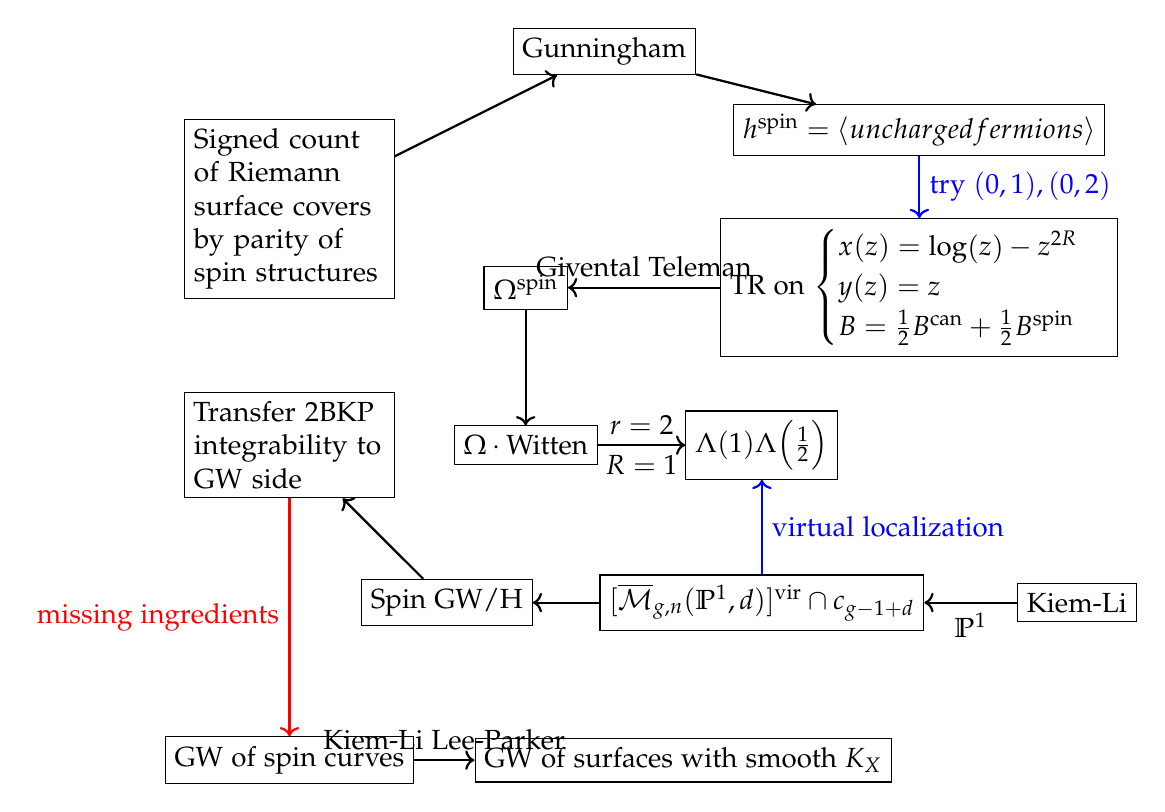
\begin{tikzpicture}[scale=1,transform shape]
    \node[draw,rectangle,text width=0.2\textwidth] (hurwitz) at (0,0) {Signed count of Riemann surface covers by parity of spin structures};
    \node[rectangle,draw] (gunningham) at (4,2) {Gunningham};
    \draw[->,thick] (hurwitz) -- (gunningham);
    \node[rectangle,draw] (operator) at (8,1) {$h^{\mr{spin}} = \ev{\Centerstack{uncharged fermions}}$};
    \draw[->,thick] (gunningham) -- (operator);
    \node[rectangle,draw] (tr) at (8,-1) {TR on $\begin{cases} x(z) = \log(z)-z^{2R} \\ y(z) = z \\ B = \frac{1}{2}B^{\mr{can}} + \frac{1}{2}B^{\mr{spin}} \end{cases}$};
    \draw[->,thick,blue] (operator) -- node[right]{\color{blue}try $(0,1), (0,2)$} (tr);
    \node[rectangle,draw] (omega) at (3,-1) {$\Omega^{\mr{spin}}$};
    \draw[->,thick] (tr) -- node[above]{\Centerstack{Givental Teleman}} (omega);
    \node[rectangle,draw] (witten) at (3,-3) {$\Omega \cdot \text{Witten}$};
    \draw[->,thick] (omega) -- (witten);
    \node[rectangle,draw] (lambda) at (6,-3) {$\Lambda(1) \Lambda\qty(\frac{1}{2})$};
    \draw[->,thick] (witten) -- node[above]{$r=2$} node[below]{$R=1$} (lambda);
    \node[rectangle,draw] (cap) at (6,-5) {$[\ol{\mc{M}}_{g,n}(\P^1,d)]^{\mr{vir}} \cap c_{g-1+d}$};
    \draw[->,blue,thick] (cap) -- node[right]{\Centerstack{virtual localization}} (lambda);
    \node[rectangle,draw] (kl) at (10,-5) {Kiem-Li};
    \draw[->,thick] (kl) -- node[below]{$\P^1$} (cap);
    \node[rectangle,draw] (gwh) at (2,-5) {\Centerstack{Spin GW/H}};
    \draw[->,thick] (cap) -- (gwh);
    \node[rectangle,draw,text width=0.2\textwidth] (bkp) at (0,-3) {Transfer $2$BKP integrability to GW side};
    \draw[->,thick] (gwh) -- (bkp);
    \node[rectangle,draw] (gw) at (0,-7) {GW of spin curves};
    \draw[->,red,thick] (bkp) -- node[left]{\Centerstack{missing ingredients}} (gw);
    \node[rectangle,draw] (surf) at (5,-7) {\Centerstack{{GW of surfaces} {with smooth $K_X$}}};
    \draw[->,thick] (gw) -- node[above]{\Centerstack{{Kiem-Li} {Lee-Parker}}} (surf);
  \end{tikzpicture}
  \caption{Summary of this chapter}
  \label{fig:summary}
\end{figure}
                          


\chapter{Teleman's classification of semisimple cohomological field theories and applications (Dimitri Zvonkine)}
\label{cha:zvonkine}

Cohomological field theories are a union of two topics:
\begin{enumerate}
\item Topological field theories (equivalently, fusion algebras or commutative Frobenius algebras);
  \item The moduli space $\ol{\mc{M}}_{g,n}$ of curves.
\end{enumerate}

\section{Topological field theories}
\label{sec:tfts}

\begin{defn}
  Let $V$ be a finite-dimensional $\C$-vector space. A \textit{topological field theory} on $V$ is a series of maps
  \[ \omega_{g,n,m} \colon V^{\otimes n} \to V^{\otimes m} \]
  satisfying the following axioms:
  \begin{enumerate}
  \setcounter{enumi}{-1}
  \item For any $g,n,m$, $\omega_{g,n,m}$ is $S_n \times S_m$-invariant;
  \item $\omega_{0,1,1} = \mr{id} \colon V \to V$;
  \item The $\omega_{g,n,m}$ satisfy the following gluing axioms: \begin{enumerate}[(a)]
    \item For any $g,n,m$,
      \[ \omega_{g,n,m} = \tr_{n+1,m+1} \omega_{g-1,n+1,m+1}. \]
    \item For any $g_1,g_2,n_1,n_2,m_1,m_2$, we have
      \[ \omega_{g_1+g_2,n_1+n_2,m_1+m_2} = \tr_{n+2+1,m_1+1} (\omega_{g_1,n_1,m_1+1} \otimes \omega_{g_2,n_2+1,m_2}). \]
    \end{enumerate}
  \end{enumerate}
\end{defn}

If we choose a basis $e_{\mu}$ of $V$, we can write a tensor $(\omega_{g,n,m})^{\nu_1, \ldots, \nu_m}_{\mu_1,\ldots,\mu_n}$. As an application of the axioms, we can see that for any $g_1, g_2$,
\[ \omega_{g_1+g_2,1,1} = \omega_{g_1,1,1} \circ \omega_{g_2,1,1}. \]

\begin{rmk}
This definition is a result of a dialogue between physicists and mathematicians and encodes (in a nice encapsulated way for mathematicians) the data of a diffeomorphism-invariant quantum field theory.
\end{rmk}

\begin{exms}\leavevmode
\begin{enumerate}[(a)]
\item Let $V = \C$. Then all $\omega_{g,n,m}$ are simply numbers. For example, we can consider $c \neq 0$ and set $\omega_{g,n,m} = c^{2-2g-n-m}$. In the case where $\dim V = 1$, this is the only example.
\item Now suppose $r \geq 1$ and set $V = \C \ev{e_0, \ldots, e_{r-1}}$. We can then solve the combinatorial problem of labelling half-edges graphs with remainders modulo $r$ such that each edge or vertex sums to $0$, and define
  \[ (\omega_{g,n,m})^{b_1,\ldots, b_m}_{a_1,\ldots,a_n} \coloneqq r^g \cdot \delta_{\sum a_i - \sum b_i \mod r}. \]
  Now consider the $2$-form $\eta \coloneqq \omega_{0,2,0} \colon V^{\otimes 2} \to \C$. Then in this example $\eta_{ab} = \delta_{a+b \mod r}$. We may also define $\eta^{\vee} \coloneqq \omega_{0,0,2}$.

\begin{prop}
$\eta$ and $\eta^{\vee}$ are inverses of each other. Here, we consider $\eta \colon V \to V^*$ and $\eta^{\vee} \colon V^* \to V$.
\end{prop}

\begin{proof}
Simply apply the gluing axiom and obtain $\omega_{0,1,1}$, which is the identity by definition.
\end{proof}

With the data of $\eta$ and $\eta^{-1}$, inputs and outputs are symmetric, so the data of a topological field theory is determined by $\omega_{g,n,0}$.

\item Let $G$ be a finite group and set $V = Z \C[G]$. We know that $V$ is spanned by conjugacy classes. Now define
  \[ \alpha \coloneqq \sum_{g_1,g_2} g_1 g_2 g_1^{-1} g_2^{-1} \in V. \]
  We can define
  \[ \omega_{g,n,0}(v_1, \ldots, v_n) \coloneqq \frac{1}{\abs{G}} [\mathbf{1}_G] v_1 \cdots v_n \cdot \alpha^g. \]
  For example, if $G = S_d$ is the symmetric group, then $V$ is spanned by partitions of $d$, and $\omega_{g,n,0}$ is a Hurwitz number.

Stepping back, note that a finite-dimensional commutative $\C$-algebra is either $\C \oplus \cdots \oplus \C$ or has at least one nilpotent element. The Burnside formula allows us to move to the idempotent basis from the usual basis 
\end{enumerate}
\end{exms}

\begin{defn}
A \textit{commutative Frobenius algebra} is a commutative associative algebra with unit $(V, \cdot, \mathbb{1})$ with a counit $\delta \colon V \to \C$ such that $\eta(u,v) \coloneqq \delta(u \cdot v)$ is nondegenerate.
\end{defn}

\begin{exm}
The ring $\C[x,y]/(x^2,xy,y^2)$ cannot be promoted to a Frobemius algebra.
\end{exm}

\begin{exm}
The counit $\delta = \frac{1}{\abs{G}}[\mathbf{1}_G](-)$ turns $V = Z \C[G]$ into a Frobenius algebra.
\end{exm}

\begin{thm}
Topological field theories are equivalent to Frobenius algebras.
\end{thm}

\begin{proof}
  Let's begin with a topological field theory. Given $V$, we can construct
  \begin{itemize}
  \item The unit as $\omega_{0,0,1}$;
  \item The counit as $\omega_{0,1,0}$;
  \item The product as $\omega_{0,2,1}$.
  \end{itemize}
  We can see that the product is associative by cutting $\omega_{0,3,1}$ in two different ways and commutative by $S_2$-equivariance of $\omega_{0,2,1}$. Clearly, $\eta = \omega_{0,2,0}$ is nondegenerate from the axioms of a TFT.

  In the other direction, we can define $\omega_{g,n,m}$ by cutting any surface into pairs of pants. We already know that pairs of pants are simply the product in the Frobenius algebra, so we get the answer. To check consistency, we can modify our decomposition and repeatedly use associativity of the Frobenius algebra.
\end{proof}

Now suppose we actually want to compute $\omega_{g,n,1}(v_1, \ldots, v_n)$ from the Frobenius algebra structure. First, we set $\alpha = \omega_{1,0,1} \in V$, and then the gluing axiom tells us that
\[ \alpha = \sum \eta^{\mu \nu} e_{\mu} \cdot e_{\nu}. \]
Then we may compute
\[ \omega_{g,n,1}(v_1, \ldots, v_n) = v_1 \cdots v_n \cdot \alpha^g. \]

\section{Moduli of curves}
\label{sec:mgn}

Recall that there is a moduli space $\mc{M}_{g,n}$ parameterizing smooth and proper curves of arithmetic genus $g$ over $\C$ with $n$ distinct (numbered) marked points whenever $2-2g-n < 0$. This has a compactification $\ol{\mc{M}}_{g,n}$ of \textit{stable curves}. Recall that a stable curve has:
\begin{itemize}
\item The only singularities allowed are nodes;
\item The marked points are all smooth;
\item The condition $2-2g-n < 0$ applies to every component if we treat all nodes and marked points as special.
\end{itemize}
Recall that $\ol{\mc{M}}_{g,n}$ is a smooth proper Deligne-Mumford stack of dimension $3g-3+n$.

\begin{exm}
  Consider the space $\mc{M}_{0,4}$. Classically, there is an isomorphism
  \[ (C,x_1,x_2,x_3,x_4) \simeq (\P^1, 0, 1, \infty, t), \]
  where
  \[ t = \frac{x_4-x_1}{x_2-x_1} : \frac{x_4-x_3}{x_2-x_3} \]
  is the cross-ratio, and thus $\mc{M}_{0,4} = \P^1 \setminus \qty{0,1,\infty}$. Compactifying, we obtain $\ol{\mc{M}}_{0,4} = \P^1$, where the points $0,1,\infty$ correspond to the $t \to 0, t \to 1, t \to \infty$ limits and are geometrically represented by curves with two components. The markings on the components are $(14)(23), (13)(24), (12)(34)$ in the three cases.
\end{exm}

We will conclude this section by giving a picture of $\ol{\mc{M}}_{g,n}$, which can be seen in~\Cref{fig:mgn}. A general point corresponds to a smooth curve, and then there are various boundary divisors corresponding to curves with nodes. There is a boundary divisor corresponding curves with non-separating nodes, and these have self-intersections which correspond to having more nodes, where the codimension is given by counting the number of nodes. The boundary is a normal crossings divisor. There are other boundary divisors which correspond to separating nodes, and they have a combinatorial description based on how the genus and marked points are split among the components.
\begin{figure}[htpb]
  \centering
  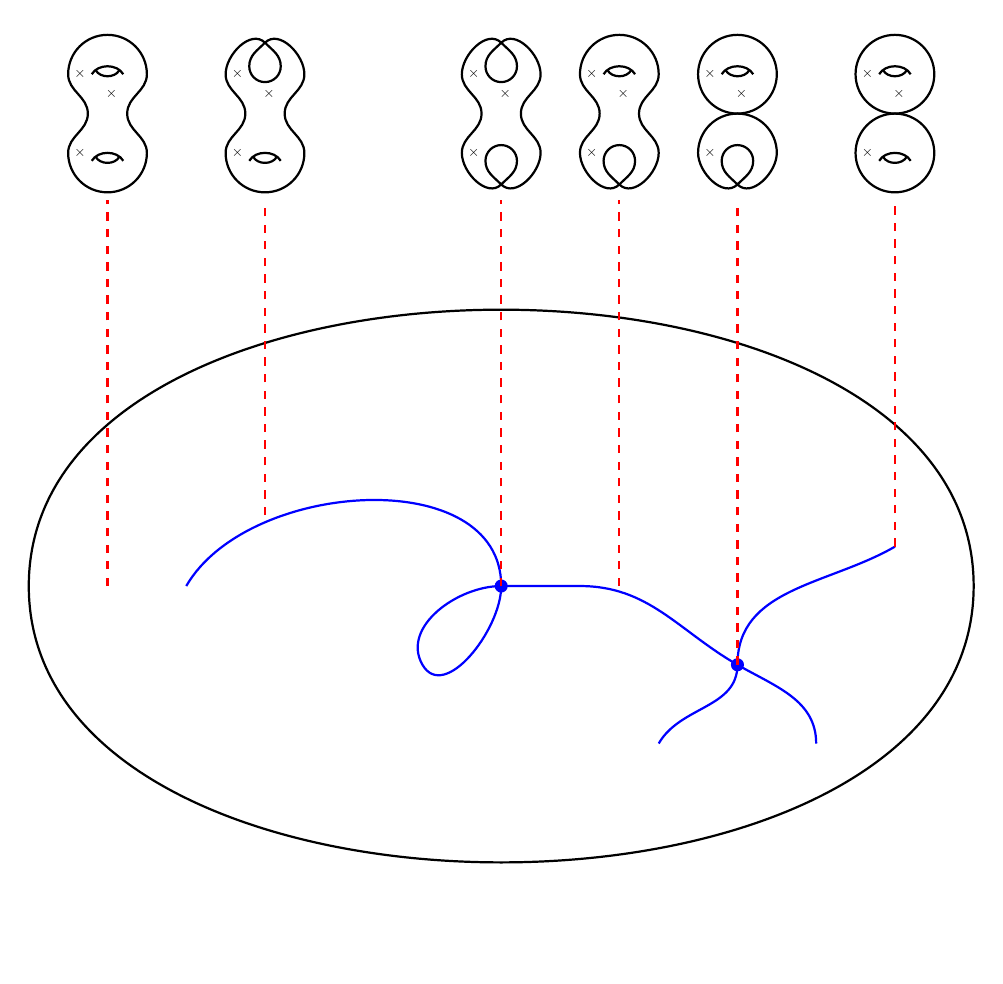
\begin{tikzpicture}[scale=1,transform shape]
    \draw[smooth,thick] (-6,0) to[out=90,in=90] (6,0) to[out=270,in=270] (-6,0);
    \draw[smooth,thick,blue] (-4,0) to[out=60,in=90] (0,0) to[out=270,in=300] (-1,-1) to[out=120,in=180] (0,0) to (1,0) to [out=0,in=150] (3,-1) to[out=330,in=90] (4,-2);
    \draw[smooth,thick,blue] (5,0.5) to[out=210,in=90] (3,-1) to[out=270,in=60] (2,-2);
    \node[fill=blue,circle,scale=0.5] at (0,0) {};
    \node[fill=blue,circle,scale=0.5] at (3,-1) {};
    \draw[dashed,thick,red] (-5,0) -- (-5,4.9);
    \draw[dashed,thick,red] (-3,0.9) -- (-3,4.9);
    \draw[dashed,thick,red] (0,0) -- (0,4.9);
    \draw[dashed,thick,red] (1.5,0) -- (1.5,4.9);
    \draw[dashed,thick,red] (3,-1) -- (3,4.9);
    \draw[dashed,thick,red] (5,0.5) -- (5,4.9);
    \draw[smooth,thick] (-5.5,5.5) to [out=270,in=180] (-5,5) to[out=0,in=270] (-4.5,5.5) to [out=90,in=270] (-4.75,6) to[out=90,in=270] (-4.5,6.5) to[out=90,in=0] (-5,7) to[out=180,in=90] (-5.5,6.5) to [out=270,in=90] (-5.25,6) to[out=270,in=90] (-5.5,5.5);
    \draw[smooth,thick] (-5.2,5.4) to[out=60,in=120] (-4.8,5.4);
    \draw[smooth,thick] (-5.15,5.45) to[out=300,in=240] (-4.85,5.45);
    \draw[smooth,thick] (-5.2,6.5) to[out=60,in=120] (-4.8,6.5);
    \draw[smooth,thick] (-5.15,6.55) to[out=300,in=240] (-4.85,6.55);
    \node[scale=0.5] at (-5.35,5.5) {$\times$};
    \node[scale=0.5] at (-5.35,6.5) {$\times$};
    \node[scale=0.5] at (-4.95,6.25) {$\times$};
    \draw[smooth,thick] (-3.5,5.5) to [out=270,in=180] (-3,5) to[out=0,in=270] (-2.5,5.5) to [out=90,in=270] (-2.75,6) to[out=90,in=270] (-2.5,6.5) to[out=90,in=45] (-3,6.9) to[out=315,in=90] (-2.8,6.6) to[out=270,in=0] (-3,6.4) to[out=180,in=270] (-3.2,6.6) to[out=90,in=225] (-3,6.9) to[out=135,in=90] (-3.5,6.5) to [out=270,in=90] (-3.25,6) to[out=270,in=90] (-3.5,5.5);
    \draw[smooth,thick] (-3.2,5.4) to[out=60,in=120] (-2.8,5.4);
    \draw[smooth,thick] (-3.15,5.45) to[out=300,in=240] (-2.85,5.45);
    \node[scale=0.5] at (-3.35,5.5) {$\times$};
    \node[scale=0.5] at (-3.35,6.5) {$\times$};
    \node[scale=0.5] at (-2.95,6.25) {$\times$};
    \draw[smooth,thick] (-0.5,5.5) to [out=270,in=225] (0,5.1) to[out=135,in=270] (-0.2,5.4) to[out=90,in=180] (0,5.6) to[out=0,in=90] (0.2,5.4) to[out=270,in=45] (0,5.1) to[out=315,in=270] (0.5,5.5) to [out=90,in=270] (0.25,6) to[out=90,in=270] (0.5,6.5) to[out=90,in=45] (0,6.9) to[out=315,in=90] (0.2,6.6) to[out=270,in=0] (0,6.4) to[out=180,in=270] (-0.2,6.6) to[out=90,in=225] (0,6.9) to[out=135,in=90] (-0.5,6.5) to [out=270,in=90] (-0.25,6) to[out=270,in=90] (-0.5,5.5);
    \node[scale=0.5] at (-0.35,5.5) {$\times$};
    \node[scale=0.5] at (-0.35,6.5) {$\times$};
    \node[scale=0.5] at (0.05,6.25) {$\times$};
    \draw[smooth,thick] (1,5.5) to [out=270,in=225] (1.5,5.1) to[out=135,in=270] (1.3,5.4) to[out=90,in=180] (1.5,5.6) to[out=0,in=90] (1.7,5.4) to[out=270,in=45] (1.5,5.1) to[out=315,in=270] (2,5.5) to [out=90,in=270] (1.75,6) to[out=90,in=270] (2,6.5) to[out=90,in=0] (1.5,7) to[out=180,in=90] (1,6.5) to [out=270,in=90] (1.25,6) to[out=270,in=90] (1,5.5);
    \draw[smooth,thick] (1.3,6.5) to[out=60,in=120] (1.7,6.5);
    \draw[smooth,thick] (1.35,6.55) to[out=300,in=240] (1.65,6.55);
    \node[scale=0.5] at (1.15,5.5) {$\times$};
    \node[scale=0.5] at (1.15,6.5) {$\times$};
    \node[scale=0.5] at (1.55,6.25) {$\times$};
    \draw[smooth,thick] (2.5,5.5) to [out=270,in=225] (3,5.1) to[out=135,in=270] (2.8,5.4) to[out=90,in=180] (3,5.6) to[out=0,in=90] (3.2,5.4) to[out=270,in=45] (3,5.1) to[out=315,in=270] (3.5,5.5) to [out=90,in=0] (3,6) to[out=180,in=90] (2.5,5.5);
    \draw[thick] (3,6.5) circle (0.5);
    \draw[smooth,thick] (2.8,6.5) to[out=60,in=120] (3.2,6.5);
    \draw[smooth,thick] (2.85,6.55) to[out=300,in=240] (3.15,6.55);
    \node[scale=0.5] at (2.65,5.5) {$\times$};
    \node[scale=0.5] at (2.65,6.5) {$\times$};
    \node[scale=0.5] at (3.05,6.25) {$\times$};
    \draw[thick] (5,5.5) circle (0.5);
    \draw[thick] (5,6.5) circle (0.5);
    \draw[smooth,thick] (4.8,6.5) to[out=60,in=120] (5.2,6.5);
    \draw[smooth,thick] (4.85,6.55) to[out=300,in=240] (5.15,6.55);
    \draw[smooth,thick] (4.8,5.4) to[out=60,in=120] (5.2,5.4);
    \draw[smooth,thick] (4.85,5.45) to[out=300,in=240] (5.15,5.45);
    \node[scale=0.5] at (4.65,5.5) {$\times$};
    \node[scale=0.5] at (4.65,6.5) {$\times$};
    \node[scale=0.5] at (5.05,6.25) {$\times$};
  \end{tikzpicture}
  \caption{Picture of $\ol{\mc{M}}_{2,3}$. The divisor with self-intersection is the image of $q \colon \ol{\mc{M}}_{1,5} \to \ol{\mc{M}}_{2,3}$ while the other divisor is the image of $s \colon \ol{\mc{M}}_{1,2} \times \ol{\mc{M}}_{1,3} \to \ol{\mc{M}}_{2,3}$.}
  \label{fig:mgn}
\end{figure}

It is important to note that the components of the boundary are given by products of smaller moduli spaces. In the boundary components with reducible curves, we can form the gluing map
\[ q \colon \ol{\mc{M}}_{g_1,n_1+1} \times \ol{\mc{M}}_{g_2, n_2+1} \to \ol{\mc{M}}_{g_1+g_2, n_1+n_2}. \]
In the components with a non-separating node, there is of course the map
\[ s \colon \ol{\mc{M}}_{g-1,n+2} \to \ol{\mc{M}}_{g,n}, \]
which is $2$-to-$1$ onto the image (since we forgot the last two markings, we can swap the two and obtain the same glued curve).

The last interesting map we should discuss are the forgetful maps
\[ p \colon \ol{\mc{M}}_{g,n+1} \to \ol{\mc{M}}_{g,n}, \]
which are defined by deleting a marked point and then stabilizing the resulting curve by collapsing rational tails (one node and either zero or one marked points) and bridges (two nodes and no marked points).

\section{Cohomological field theories}
\label{sec:cohft}

\begin{defn}
  Let $V$ be a finite-dimensional $\C$-vector space. A \textit{cohomological field theory} on $V$ is the data of a unit vector $0 \neq \mathbb{1} \in V$, a nondegenerate symmetric bilinear form $\eta$, and a collection
  \[ (\Omega_{g,n} \colon V^{\otimes n} \to H^{*}(\ol{\mc{M}}_g,n))_{2-2g-n < 0} \]
  satisfying the following axioms:
  \begin{enumerate}
    \setcounter{enumi}{-1}
  \item Each $\Omega_{g,n}$ is $S_n$-equivariant, where $S_n$ acts on $\ol{\mc{M}}_{g,n}$ by permuting the marked points (here, we will only consider the even part of the cohomology of $\ol{\mc{M}}_{g,n}$);
  \item For all $u, v \in V$, $\Omega_{0,3}(u,v,\mathbb{1}) = \eta(u,v)$;
  \item We have the following gluing axioms: \begin{enumerate}[(a)]
    \item For any $g,n$, we have
      \[ s^* \Omega_{g,n}(v_1 \otimes \cdots \otimes v_n) = \Omega_{g-1,n+1}(v_1 \otimes \cdots \otimes v_n \otimes \eta^{-1}). \]
    \item Choose a basis $(e_{\mu})$ for $V$. Then we have
      \[ q^* \Omega_{g,n}(v_1, \ldots, v_n) = \sum_{\mu,\nu} \Omega_{g_1,n_1+1}(v_1, \ldots,v_n, e_{\mu}) \times \eta^{\mu\nu} \times \Omega_{g_2, n_2+1}(v_{n_1+1}, \ldots, v_n, e_{\nu}). \]
    \end{enumerate}
  \item (Optional, flat unit, string equation) For any $g, n$, we have
    \[ p^*\Omega_{g,n}(v_1, \ldots, v_n) = \Omega_{g,n+1}(v_1, \ldots, v_n, \mathbb{1}). \]
  \end{enumerate}
\end{defn}

We will now give several examples of cohomological field theories.\footnote{Dimitri claims that all examples of cohomological field theories are intimidating.}

\begin{defn}
  Recall that if $\mc{C} \xrightarrow{\pi} \ol{\mc{M}}_{g,n}$ is the universal curve, then there is a sheaf
  \[ \mathbb{E} \coloneqq \pi_* \omega_{\pi} \]
  on $\ol{\mc{M}}_{g,n}$. Above any stable curve $C$, the fiber is simply $H^0(\omega_C)$. Recall that because nodes are Gorenstein, $\omega_C$ is a line bundle. In the more analytic setting, the sections are \textit{abelian differentials}, which are simply meromorphic $1$-forms on each component with poles allowed only at the nodes and opposite residues on the branches. By Serre duality, connectedness, and flatness, $\mathbb{E}$ is a vector bundle of rank $g$, called the \textit{Hodge bundle}.
\end{defn}

\begin{thm}\label{thm:lambdag}
  If we set $V = \C$, $\mathbb{1} = 1$, $\eta = (1)$, and
  \[ \Omega_{g,n}(1, \ldots, 1) = c(\mathbb{E}_g), \]
  we obtain a cohomological field theory.
\end{thm}

\begin{proof}
  The first two axioms are clearly satisfied, so we check the gluing axioms. We will first show that
  \[ q^* c(\mathbb{E}_g) = c(\mathbb{E}_{g_1}) c(\mathbb{E}_{g_2}). \]
  Because poles are not allowed at the node (by the residue formula), we have $q^* \mathbb{E}_g = \mathbb{E}_{g_1} \oplus \mathbb{E}_{g_2}$. By the splitting axiom for the total Chern class, we are done. We now turn to showing that
  \[ s^* c(\mathbb{E}_g) = c(\mathbb{E}_{g-1}). \]
  There is an exact sequence
  \[ 0 \to \mathbb{E}_{g-1} \to s^* \mathbb{E}_g \to \mc{O} \to 0 \]
  given by $\alpha \mapsto \Res_{n+1} \alpha$, so by the trivial bundle axiom for the total Chern class, we are done. In fact, the string equation is also satisfied because $\E$ does not depend on the marked points.
\end{proof}

\begin{rmk}
For any CohFT, if we restrict $\Omega_{g,n}$ to the $H^0(\ol{\mc{M}}_{g,n}) = \C$, we obtain a topological field theory.
\end{rmk}

\begin{rmk}
  For any $a_i$, we may consider any characteristic class of the form
  \[ \exp \qty(\sum a_i \on{ch}_i(\mathbb{E}_g)) \]
  and obtain a CohFT.
\end{rmk}

\begin{defn}
Let $(C, x_1, \ldots, x_n)$ be a smooth curve with marked points and $K_C$ be the cotangent bundle. Then an \textit{$r$-spin structure} on $C$ is a line bundle $\mc{L}$ with an isomorphism $\mc{L}^{\otimes r} \simeq K_C\qty(-\sum a_i x_i)$, where $a_1, \ldots, a_n \in \qty{0, \ldots, r-1}$. Now note that if we fix the $a_i$, then there are $r^{2g}$ possible choices of $\mc{L}$ corresponding to the possible choices of $r$-torsion in $\Pic(C)$.
\end{defn}

We now obtain a moduli space $\mc{M}_{g;a_1,\ldots,a_n}^{1/r}$ with an \'etale map
\[ \mc{M}_{g;a_1,\ldots,a_n}^{1/r} \xrightarrow{r^{2g}:1} \mc{M}_{g,n}. \]
We can compactify this to $\ol{\mc{M}}_{g;a_1,\ldots,a_n}^{1/r}$, but now the map to $\ol{\mc{M}}_{g,n}$ is ramified at the boundary. Then we may define Witten's class on $\ol{\mc{M}}_{g;a_1,\ldots,a_n}^{1/r}$ and push it forward to $\ol{\mc{M}}_{g,n}$.

We may now set $V = \C\ev{e_0, \ldots, e_{r-2}}$, write $\mathbb{1} = e_0$, and set $\eta_{ab} = \delta_{a+b,r-2}$ to be the antidiagonal form. Then we will set $\Omega_{g,n}(e_{a_1}, \ldots, e_{a_n})$ to be Witten's class. This is a cohomological field theory.

\begin{defn}
  Suppose that $h^0(C, \mc{L}) = 0$ (this only happens in genus $0$). Then if $\pi \colon \mc{C} \to \ol{\mc{M}}_{g;a_1,\ldots,a_r}^{1/r}$ is the universal curve, $R^1 \pi_* \mc{L}$ is a vector bundle. Then we may define the \textit{Witten class}
  \[ W_{g;a_1,\ldots,a_n} \coloneqq e(V^*). \]
  In the complicated case when $h^0$ doesn't vanish, the Witten class may be defined using cosection localization. In our situation, let $X$ be the space of sections of $\mc{L}$. Then if $s \in \Gamma(C, \mc{L})$, we have
  \[ s^{r-1} \in \Gamma(C, \mc{L}^{\otimes r-1}) = \Gamma\qty(C, K\qty(-\sum a_i x_i) \otimes \mc{L}^*) = H^1(C, \mc{L})^* = V^*, \]
  which gives us $s^{r-1} \colon V \to \mc{O}$.
\end{defn}

\begin{rmk}
  Suppose $\sigma L \to \mc{O}$ is a (meromorphic) cosection. Then we can consider $c_1(L) = P-Z$, so in the case of an obstruction bundle $V$ and a cosection $L \to \mc{O}$, we may consider $[X] \cap c_1(L) \cdot e(V)$. For example, if we consider
  \[\sigma \colon \C^2 \xrightarrow{ax+by} \to \C \]
  over $\C^2_{x,y}$, $\sigma$ is surjective except over $(x,y) = (0,0)$. We can then blow up to obtain the situation of $V \oplus L$.
\end{rmk}

\begin{exm}
  These Witten classes can be hard to compute, but there are some relatively simple examples. First, there is
  \[ W_{0,3}(a_1,a_2,a_3) = \begin{cases}
                               1 & a_1 + a_2 + a_3 = r-2 \\
                               0 & \text{otherwise},
                             \end{cases} \]
  and a second relatively accessible example is
  \[ W_{0,4}(a_1, a_2, a_3,a_4) = \begin{cases}
                                    1 & a_1+a_2+a_3+a_4 = r-2, \text{ other conditions} \\
                                    \frac{1}{r} \min(a_i,r-1-a_i) & a_1+a_2+a_3 + a_4 = 2r-2 \\
                                    0 & \text{otherwise}.
                                  \end{cases} \]
\end{exm}

For the final example, let $\g$ be a simple Lie algebra, for example $\mf{sl}_N$. Then let $G$ be the compact real form of the Lie group associated to $\g$, for instance $SU_N$. Then let $T \subseteq G$ be the maximal torus with Lie algebra $\mf{t}$. Then we may consider positive weights, which in the case of $\mf{sl}_N$ are parameterized by Young diagrams of length at most $N-1$. We will define the \textit{level} $\ell$ to be all partitions with width at most $\ell$. We will then set the data
\begin{align*}
  V &= \C \ev{e_{\mu}}_{\text{level } \ell}, \\
  \mathbb{1} &= e_0, \\
  \eta_{\mu\nu} &= \delta_{\mu,\nu^*},
\end{align*}
where $\mu^*$ is the complement of $\mu$ in an $N \times N$ square (corresponding to the adjoint representation).

\begin{exm}
In the simplest example, irreducible representations of $SU_2$ are given by integers (or really weights on the half-line). They are really just $\on{Sym}^n \C^2$, where $\C^2$ is the defining representation.
\end{exm}

We will now construct the \textit{Verlinde bundle} $\mathbb{V}$ on $\ol{\mc{M}}_{g,n}$. We will do the construction for $U(1) = S^1$ (although this will break down) and for a simple group $G$. 
\begin{table}[htpb]
  \centering
  \caption{Construction of Verlinde bundle}
  \label{tab:verlinde}
  \begin{tabular}{p{0.45\textwidth}p{0.45\textwidth}}
    \toprule
    $U(1) = S^1$ & Simple group $G$ \\
    \midrule
    Curve $C$ & Curve $(C, x_1, \ldots, x_n)$ \\
    $\on{Jac}(C)$ parameterizing flat connections on $C \times U(1)$ & Moduli space $\mc{M}$ of flat connections on $C \times G$ with monodromies $\exp(\mu_i/\ell)$ at $x_i$. \\
    $\omega = [\Theta]$ & Canonical symplectic form $\omega$ \\
    Line bundle $\mc{L} = \mc{O}(\ell \Theta)$ on $\mr{Jac}(C)$ & Line bundle $\mc{L}$ on $\mc{M}$ such that $c_1(\mc{L}) = \ell \omega$ \\
    Vector bundle $H^0(\on{Jac}(C), \ell)$ of $\theta$-functions of weight $\ell$ & Vector bundle $\mathbb{V}_C = H^0(\mc{M}, \mc{L})$ \\
    \bottomrule
  \end{tabular}
\end{table}

We have defined a vector bundle $\mathbb{V}$ on $\mc{M}_{g,n}$, which by a theorem of Faltings extends to $\ol{\mc{M}}_{g,n}$ as a vector bundle. Then there are the formulae
\begin{align*}
  q^* \mathbb{V}_{g,n}(\mu_1, \ldots, \mu_n) &= \bigoplus_{\mu} \qty[\mathbb{V}_{g_1,n_1+1}(\mu_1, \ldots, \mu_{n_1},\mu)\otimes \mathbb{V}_{g_2,n_2+1}(\mu_{n_1+1}, \ldots, \mu_n, \mu^*)] \\
  s^* \mathbb{V}_{g,n}(\mu_1, \ldots, \mu_n) &= \bigoplus_{\mu} \mathbb{V}_{g-1,n+2}(\mu_1, \ldots, \mu_n, \mu, \mu^*).
\end{align*}
These imply that taking $\ch(\mathbb{V}_{g,n})$ is a cohomological field theory.

\begin{rmk}
It is in extending to $\ol{\mc{M}}_{g,n}$ where the construction for $U(1)$ breaks down because line bundles have degrees, and when we degenerate a bundle of degree $0$, the two components could have nonzero degrees.
\end{rmk}

\begin{rmk}
The topological part of this cohomological field theory is simply $\ch_0(\mathbb{V}) = \on{rk}(\mathbb{V})$ and is given by the Verlinde formula (using the idempotents of the Frobenius algebra).
\end{rmk}

\section{Givental group action}
\label{sec:givental_group}

\subsection{Stable graphs}
\label{subsec:stable_graphs}

Recall our picture~\Cref{fig:mgn} of $\ol{\mc{M}}_{g,n}$. If $\pi \colon \mc{C} \to \ol{\mc{M}}_{g,n}$ is the univeral curve and $s_i \colon \ol{\mc{M}}_{g,n} \to \mc{C}$ is the section corresponding to the $i$-th marked point, we may construct the line bundle
\[ \mathbb{L}_i \coloneqq s_i^* \omega_{\pi} \]
corresponding to the $i$-th cotangent line. Then we define the \textit{psi-classes}
\[ \psi_i = c_1(\mathbb{L}_i) \in H^2(\ol{\mc{M}}_{g,n}). \]
The boundary strata correspond to \textit{stable graphs} which have vertices corresponding to components, edges corresponding to nodes, and half edges (legs) corresponding to marked points. Each vertex is labelled with a nonnegative integer corresponding to a genus, and each leg is labelled with a number. An example is displayed in~\Cref{fig:stablegraph}.

\begin{figure}[htpb]
  \centering
  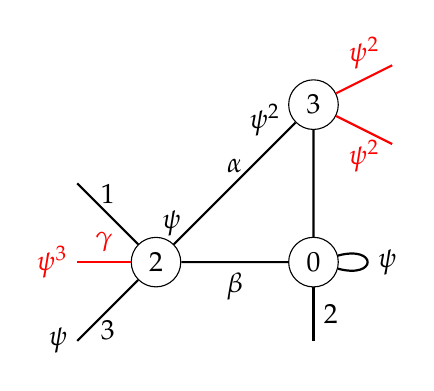
\begin{tikzpicture}[scale=1,transform shape,every loop/.style={}]
    \node[circle,draw] (A) at (0,0) {$2$};
    \node[circle,draw] (B) at (2,2) {$3$};
    \node[circle,draw] (C) at (2,0) {$0$};
    \draw[thick] (A) -- node[above]{$\alpha$} (B) -- (C) -- node[below]{$\beta$} (A);
    \draw[thick] (A) -- node[below]{$3$} (-1,-1);
    \draw[thick,red] (A) -- node[above]{$\gamma$} (-1,0);
    \draw[thick] (A) -- node[above]{$1$} (-1,1);
    \draw[thick,red] (B) -- node[above]{$\psi^2$} (3,2.5);
    \draw[thick,red] (B) -- node[below]{$\psi^2$} (3,1.5);
    \draw[thick] (C) -- node[right]{$2$} (2,-1);
    \draw[thick] (C) edge[loop right] node[right] {$\psi$} (C);
    \node[red,anchor=east] at (-1,0) {$\psi^3$};
    \node[anchor=east] at (-1,-1) {$\psi$};
    \node[anchor=east] at (1.7,1.8) {$\psi^2$};
    \node[anchor=south] at (0.2,0.2) {$\psi$};
  \end{tikzpicture}
  \caption{Example of a stable graph in $\ol{\mc{M}}_{7,3}$ and associated tautological class. Red half edges are forgotten from larger moduli spaces. This stable graph describes the image of a map
    $\ol{\mc{M}}_{2,4+\color{red} 1} \times \ol{\mc{M}}_{3,2+\color{red} 2} \times \ol{\mc{M}}_{0,5} \to \ol{\mc{M}}_{2,4} \times \ol{\mc{M}}_{3,2} \times \ol{\mc{M}}_{0,5} \to \ol{\mc{M}}_{7,3}$.}
  \label{fig:stablegraph}
\end{figure}

For the forgetful morphism $p \colon \ol{\mc{M}}_{g,n+1} \to \ol{\mc{M}}_{g,n}$, we may define the \textit{kappa-class}
\[ \kappa_m \coloneqq p_* \psi_{n+1}^{m+1}. \]
Then the \textit{tautological classes} are those which can be obtained from $1$ using the maps $p,q,s$.

\subsection{Group action on cohomological field theories}
\label{subsec:group_action}

Define the formal variable
\[ T = t_2 \psi^2 + t_3 \psi^3 + \cdots \in \psi^2 V[[\psi]], \]
where $t_i \in V$. Then we define
\[ (T\Omega)_{g,n}(v_1, \ldots, v_n) \coloneqq \sum_{m\geq 0} \frac{1}{m!} (p_m)_* \Omega_{g,n+m}(v_1, \ldots, v_n, T(\psi_{n+1}), \ldots, T(\psi_{n+m})). \]
Composing these translations corresponds to addition of power series. If we consider the action $T_a+T_b$, we see that adding $m_a$ copies of $T_a$ and $m_b$ copies of $T_b$ gives us a leading coefficient of
\[ \frac{1}{m!} \frac{m!}{m_a!m_b!} = \frac{1}{m_a! m_b!}. \]
We may check that $T$ preserves the gluing axiom, but nodes are always glued using $\eta^{-1}$, so we are fine. The only thing that is not preserved is the string equation (or flat unit).

We will also consider operators
\[ R(\psi) = \mr{Id} + R_1 \psi + R_2 \psi^2 + \cdots \in \End(V)[[\psi]]. \]
These are required to satisfy the symplectic condition
\[ R(\psi) \cdot R^*(-\psi) = \mr{Id}, \]
where the adjoint is taken with respect to $\eta$. Now define the cohomological field theory $(R\Omega)_{g,n}(v_1,\ldots,v_n)$ as a sum over stable graphs $\Gamma$ of genus $g$ with $n$ legs of $\Omega$ modified by the following procedure in~\Cref{fig:contribution}:
\begin{itemize}
\item At every vertex, place a copy of $\Omega$;
\item For any leg corresponding to the $i$th marked points, insert $R^{-1}(\psi_i)v_i$;
\item At any edge, insert a copy of
  \[ \Delta = \frac{\eta^{-1} - R^{-1}(\psi')\eta^{-1} R^{-1}(\psi'')^t}{\psi' + \psi''}, \]
  where $\psi', \psi''$ are the $\psi$-classes at the two components of the node.
\item Divide by $\abs{\Aut \Gamma}$.
\end{itemize}
\begin{figure}[htpb]
  \centering
  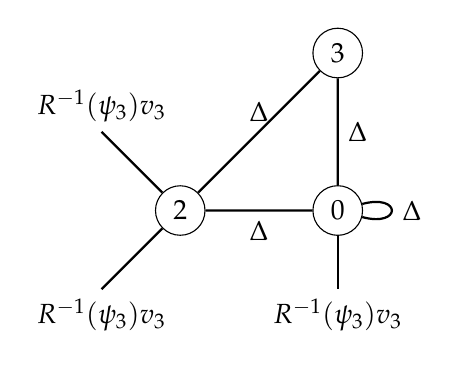
\begin{tikzpicture}[scale=1,transform shape,every loop/.style={}]
    \node[circle,draw] (A) at (0,0) {$2$};
    \node[circle,draw] (B) at (2,2) {$3$};
    \node[circle,draw] (C) at (2,0) {$0$};
    \draw[thick] (A) -- node[above]{$\Delta$} (B) -- node[right]{$\Delta$} (C) -- node[below]{$\Delta$} (A);
    \draw[thick] (A) -- (-1,-1);
    \draw[thick] (A) -- (-1,1);
    \draw[thick] (C) -- (2,-1);
    \draw[thick] (C) edge[loop right] node[right] {$\Delta$} (C);
    \node[anchor=north] at (-1,-1) {$R^{-1}(\psi_3)v_3$};
    \node[anchor=south] at (-1,1) {$R^{-1}(\psi_3)v_3$};
    \node[anchor=north] at (2,-1) {$R^{-1}(\psi_3)v_3$};
  \end{tikzpicture}
  \caption{Contribution of a stable graph to $R\Omega$}
  \label{fig:contribution}
\end{figure}

We need to prove that:
\begin{enumerate}
\item This gives a group action: $R_a(R_b \Omega) = (R_aR_b)\Omega$;
\item If $T_b = R T_a$, then $R(T_a\Omega) = T_b (R\Omega)$;
\item This $R\Omega$ is a cohomological field theory.
\end{enumerate}

This is complicated, so we will restrict ourselves to computing $q^*(R\Omega)$. Recall that $q$ corresponds to creating a new edge, so if $\Gamma$ does not have an edge separating the curve into curves which can be glued by $q$, we create a new edge and insert $\eta^{-1}$. If the edge is already present, then the normal line bundle to the boundary divisor corresponding to $q$ has $c_1 = -( \psi' + \psi'' )$, so we replace $\Delta$ with
\[ \Delta \cdot c_1(\mc{N}) = -\Delta (\psi' + \psi''). \]
We therefore sum over all contributions to obtain
\[ \eta^{-1} - (\psi' + \psi'') \Delta = R^{-1} (\psi') \eta^{-1} R^{-1}(\psi'')^t. \]
This is precisely what is needed to satisfy the gluing axiom.

\section{Teleman's classification}
\label{sec:teleman}

We are now ready to formulate Teleman's theorem.
\begin{thm}[Teleman]
  Let $\Omega$ be a cohomological field theory, $\omega$ be its topological part, and assume that the Frobenius algebra corresponding to $\omega$ is semisimple. Then there exists a unique $T \in \psi^2 V[[\psi]], R \in \End(V)[[\psi]]$ such that
  \[ \Omega = R T \omega. \]
  Moreover, $\Omega$ satisfies the string equation if and only if
  \begin{align*}
    T &= \psi(\mathbb{1} - R(\mathbb{1}))\psi \\
      &= -R_1(\mathbb{1}) \psi^2 - R_2(\mathbb{1})\psi^3 - \cdots,
  \end{align*}
  which is equivalent to the condition that $RT$ preserves the vector $-\mathbb{1} \psi$.
\end{thm}

\begin{rmk}
The condition of preserving $-\mathbb{1}\psi$ is the same as preserving the vertex of Givental's Lagrangian cone, which is the \textit{dilaton shift} $-\mathbb{1}\psi$.
\end{rmk}

We are now ready to return to our examples.
\begin{enumerate}[(a)]
\item In the case of the Hodge bundle $\mathbb{E}$, the $R$-matrix is given by
  \[ R(\psi) = \exp\qty[\sum_{m\geq 1} \frac{B_{m+1}}{m(m+1)} (-\psi)^m], \]
  where $B_{m+1}$ is the Bernoulli number. This is computed using Mumford's formula, which computes the Chern characters of $\mathbb{E}$. For example,
  \begin{align*}
    \lambda_1 &= c_1(\mathbb{E}) \\
    &= \frac{1}{12}\qty(\kappa_1 = \sum \psi_i + \delta),
  \end{align*}
  where $\delta$ is the sum of all boundary divisors.
\item We will now consider Witten's $3$-spin class. In this case
  \[ V = \ev{e_0, e_1}, \qquad \mathbb{1} = e_0, \qquad \eta = \mqty(0 & 1 \\ 1 & 0). \]
  The product is given by
  \[ W_{0,3}(a_1,a_2,a_3) = \begin{cases}
                              1 & \sum a_i = 1 \\
                              0 & \text{otherwise},
                            \end{cases}
                          \]
  and therefore the only nonzero element is $W_{0,3}(0,0,1) = 1$. Therefore, the product is given by:
  \begin{align*}
    e_0 \cdot e_0 &= e_1^* = e_0 \\
    e_0 \cdot e_1 &= e_0^* = e_1 \\
    e_1 \cdot e_1 &= 0.
  \end{align*}
  Because $e_1$ is nilpotent (in fact the algebra is $\C[x]/x^2$), we are not semisimple. The solution to this is to shift the Witten class by $3e_1$ to obtain
  \begin{align*}
\wt{W}_{g,n}(a_1, \ldots, a_n) \coloneqq \sum_{m\geq 0} \frac{3^m}{m!} (p_m)_* W_{g,n+m}(a_1, \ldots, a_n, 1, \ldots, 1).
  \end{align*}
  This brings us to a semisimple point in the Frobenius manifold, where we also have
  \[ \wt{W}_{0,3} (1,1,1) = p_* W_{0,4}(1,1,1,1) = 1 \]
  and thus the product is modified to have
  \[ e_1 \cdot e_1 = e_0. \]
  It is easy to see that the algebra is $\C[x]/(x^2-1)$ and the idempotents are
  \[ \frac{e_0+e_1}{2}, \frac{e_0-e_1}{2}. \]
  The shifted Witten class is no longer of pure degree, but the correction terms have lower degrees of the same parity.

  We may now apply the classification theorem. From the product and the quadratic form, the topological part is
  \[ \omega_{g,n}(a_1, \ldots, a_n) = 2^g \cdot \delta_{\sum a_i + g+1 \mod 2}. \]
  We can now write the $R$-matrix. First, define the power series (asymptotic expansions of the Airy function)
  \begin{align*}
    A(\psi) &= \sum_{m\geq 0} \frac{(6m)!}{(2m)!(3m)!} \qty(-\frac{\psi}{1728})^m \\
    B(\psi) &= \sum_{m\geq 0} \frac{1+6m}{1-6m} \frac{(6m)!}{(2m)!(3m)!} \qty(-\frac{\psi}{1728})^m.
  \end{align*}
  Now set
  \[ R^{-1} = \mqty(A^{\mr{even}} & B^{\mr{odd}} \\ A^{\mr{odd}} & B^{\mr{even}}). \]
  If we extract the part of degree $\frac{g-1+\sum a_i}{3}$, we obtain a formula for Witten's class, and if we consider the higher degree parts, we obtain tautological relations on the moduli space of curves. The simplest tautological relation is the WDVV equation on $\ol{\mc{M}}_{0,4}$. A new relation, due to Getzler, lives on $\ol{\mc{M}}_{1,4}$. If we consider the simpler case of $\mc{M}_g$, then there are no relations between the $\kappa_i$ up to degree $\frac{g}{3}$. There is a conjecture that all tautological relations come from Witten's class, and for example, if we consider the degree $2$ part of the $g=1,n=4,a_1 = \cdots a_4$ case, we obtain Getzler's relation.
\item We now consider the Verlinde bundle for $\mf{sl}_2(\C)$ at level $\ell = 1$. There are only two representations $e_{\emptyset} = \mathbb{1}, e_{\square}$, and $\eta$ is diagomal. Then the Verlinde bundle is a pullback except in the case
  \begin{align*}
\on{ch}\qty(\mathbb{V}_{g,n}(\square, \ldots, \square)) &= e^{-\frac{\lambda_1}{2}} \sum_{\Gamma} \cdot \frac{2^{g-h^1(\Gamma)}}{\abs{\Aut \Gamma}} \cdot \text{contribution},
  \end{align*}
  where $\Gamma$ runs over stable graphs with vertices of even degree. The contribution of $\Gamma$ is given by inserting $e^{-\frac{\psi_i}{4}}$ at marked points and inserting
  \[ \Delta = \frac{1-e^{-\frac{\psi'+\psi''}{4}}}{\psi' + \psi''} \]
  at the edges.
\end{enumerate}

\section{Relation to topological recursion}
\label{sec:relation_tr}

Consider a disk near $x_i$ with simple ramification, so we have the coordinate $z_i = \sqrt{x-x_i}$. Recall from~\Cref{defn:tr} that topological recursion requires the specification of the data $y_i(z)$ for all $i$, the Bergman kernel $B(z_i,z_j) \dd{z_i} \dd{z_j}$ for all $i, j$, and the series $\xi_i(x)$.

Applying the Laplace transform, we obtain $T(\psi)$ and $\Delta(\psi',\psi'')$ in place of $y$ and $B$ (which yield $\Omega$), where we drop even powers of $z$ and send
\[ a_{2k+1} z^{2k+1} \rightsquigarrow \frac{a_{2k+1}}{(2k+1)!!} \psi^k. \]
Then topological recursion produces forms given by
\[ \sum \int \Omega_{g,n} \psi_1^{k_1} \cdots \psi_n^{k_n} \prod \xi_i^{(k_i)}(x_i). \]



\end{document} 

%%% Local Variables:
%%% mode: latex
%%% TeX-master: t
%%% End:
